\documentclass[11pt,a4paper]{article}

\usepackage{graphicx}
\graphicspath{{Figuras/}}

\usepackage[utf8]{inputenc}
\usepackage[spanish,es-tabla]{babel}
\usepackage[left=2.5cm,right=2.5cm,bottom=2cm,top=2.5cm]{geometry}
\usepackage{titling}
\usepackage{bm}
\usepackage{multirow}
\usepackage{floatrow}
\newfloatcommand{capbtabbox}{table}[][\FBwidth]
\usepackage[table,xcdraw]{xcolor}

\usepackage{blindtext}
\usepackage{verbatim}
\usepackage{amsmath}
\usepackage{amssymb}
\usepackage{textcomp}
\usepackage{bbm}
\usepackage{multicol}
\usepackage{enumitem}
\usepackage{array}
\usepackage{booktabs}
\usepackage{placeins}
\usepackage[hidelinks]{hyperref}

\usepackage[separate-uncertainty = true]{siunitx}
\sisetup{output-decimal-marker = {,}, per-mode=fraction, exponent-product = \cdot}

% Renombre para titulo de referencias / bibliografía
\renewcommand\refname{}

% Bullets para las listas
\renewcommand{\labelitemi}{$\bullet$}
\makeatletter
\def\namedlabel#1#2{\begingroup
    #2%
    \def\@currentlabel{#2}%
    \phantomsection\label{#1}\endgroup}
\makeatother

% Numeración anidada con números
\renewcommand{\labelenumii}{\arabic{enumi}.\arabic{enumii}}
\renewcommand{\labelenumiii}{\arabic{enumi}.\arabic{enumii}.\arabic{enumiii}}
\renewcommand{\labelenumiv}{\arabic{enumi}.\arabic{enumii}.\arabic{enumiii}.\arabic{enumiv}}

\newcommand{\paralelo}{\mathbin{\!/\mkern-5mu/\!}}
\sisetup{exponent-product=\cdot, output-decimal-marker={,}, per-mode=symbol}

\usepackage{fancyhdr}
\usepackage[T1]{fontenc}
\pagestyle{fancy}
\fancyhf{}
\lhead{\textit{Sistema de Aislado Limitado / Total (SAL/T)}}
\rhead{\textit{UBA - Facultad de Ingeniería}}
\cfoot{\thepage}

\setlength{\headheight}{13.6pt}

% Figuras con numeración por sección, subsección o continuo
%\counterwithout{figure}{section}
\counterwithin{figure}{section}
%&\counterwithin{figure}{subsection}

\usepackage{changepage}
%%%%%%%%%%%%%%%%%%%%%%%%%%%%%%%%%%%%%%%%%%%


\begin{document}

\pagenumbering{gobble}
\DeclareSIUnit{\div}{div}
\DeclareSIUnit{\Sa}{Sa}

\begin{titlepage}	
	\centering

	%\vspace*{0.3cm}	

%     \Large{\textsc{Universidad de Buenos Aires}}\\ 
%	\Large{\textsc{Facultad de Ingeniería}}\\ 
%	\vspace*{1cm}	

	\begin{figure}[h]
		\centering
		
\includegraphics[scale=1]{img/logo_fiuba_new.pdf} 	
	\end{figure}
	\vspace*{2cm}

\huge{\textsc{86.00 Tesis de Ingeniería Electrónica - Informe de tesis\\}}\vspace{.3cm}
	
	\newcommand{\LargoDeBarra}{1}  % Ajustar
	
	\rule{\LargoDeBarra\linewidth}{0.3 mm} \\[0.1 cm]
	\LARGE{\textbf{Rediseño e implementación de un Sistema de Aislado Limitado / Total (SAL/T) para trenes}} \\[-0.3 cm]
	\rule{\LargoDeBarra\linewidth}{0.3 mm}

\vspace*{2cm}

    \begin{table}[htb]
%    \raggedright

    \begin{tabular}{lcc} 
        \textbf{Autor}              &     &     \\
        Anus, Martín     &    manus@fi.uba.ar & padron n° 101033   \\
        & & \\
         \textbf{Directores de tesis} &         &   \\
         Lutenberg, Ariel       & alutenb@fi.uba.ar & Director  \\
         Gomez, Pablo       & pgomez@fi.uba.ar   & Co-director \\
        Laiuppa, Adrián      & alaiuppa@gmail.com & Co-director     \\
        & &  \\
         \textbf{Jurados}        & \\
         Cruz, Juan Manuel       & jcruz@fi.uba.ar   & \\
         Germino, Santiago        & sgermino@fi.uba.ar   & \\
         Menéndez, Martín        & mmenendez@fi.uba.ar   & 
        \end{tabular}
     \end{table}



\vspace*{1cm}
	

\textit{\large{Este trabajo fue realizado en la Ciudad Autónoma de Buenos Aires,}} \\
\textit{\large{entre agosto de 2023 y diciembre de 2024.}}

\end{titlepage}

\newpage

\vspace*{\fill}

\begin{center}

{\huge \textit{Resumen}}


\vspace{1.5cm}

\begin{adjustwidth}{2cm}{2cm}
\begin{center}
    

        
Este trabajo presenta el diseño e implementación de un prototipo para un sistema de aislado limitado total para formaciones ferroviarias (SAL/T) basado en un pliego de especificaciones de la empresa Trenes Argentinos Operaciones y en una primera versión del prototipo realizado anteriormente en el contexto del Grupo de Investigación en Calidad y Seguridad de las Aplicaciones Ferroviarias (GICSAFe). En esta versión, se agregan nuevas funcionalidades, se actualiza el hardware utilizado y se mejora la portabilidad de su firmware. \\

\vspace{.8cm}

Este sistema permite aumentar la seguridad de los trenes ante una falla en alguno de sus sistemas instrumentados de seguridad interfiriendo las señales de corte de tracción y freno de emergencia de la formación y aislando el subsistema en fallo. El SAL/T considera múltiples fuentes de medición de la velocidad de la formación y la comunicación con una central operativa para determinar cómo debe intervenir estas señales críticas para llevar a la formación a un estado seguro de manera controlada.  \\ 

\vspace{.8cm}

A lo largo del proyecto, se aplicaron conocimientos de electrónica general, diseño de circuitos, diseño de placas impresas, utilización de protocolos de comunicación e implementación de firmware basado en sistemas operativos en tiempo real.


\end{center}
\end{adjustwidth}

\end{center}

\vspace{8cm}

\vspace*{\fill}


\newpage

\vspace*{\fill}

\begin{center}

{\huge \textit{Agradecimientos}}


\vspace{1.3cm}

\begin{adjustwidth}{2cm}{2cm}
\begin{center}
        
Quiero expresar mi agradecimiento a los directores de esta tesis; Ariel, Pablo y Adrián por su constante apoyo, motivación, ayuda y guía que me brindaron a lo largo de este proyecto. \\ 
\vspace{.7cm}

Al grupo de investigación GICSAFe que me introdujo en el mundo de los sistemas ferroviarios y me abrió la posibilidad de desarrollar este trabajo sobre las sólidas bases de conocimiento del grupo.

\vspace{.7cm}

A las personas de la empresa Trenes Argentinos que dedicaron su tiempo para definir el objetivo y el alcance de este proyecto. 

\vspace{.7cm}

Al ingeniero Iván Di Vito por dejar una versión anterior de este sistema de una calidad enorme.

\vspace{.7cm}

A todos los docentes que tuve a lo largo de mi vida por formarme como profesional y como persona. 

\vspace{.7cm}

Al arquitecto Martín Mendilaharzu por la ayuda en el diseño y fabricación del gabinete. 

\vspace{.7cm}

A Carlos, mi papá, por mostrarme la ingeniería en todos los detalles de la vida y contagiarme su pasión.

\vspace{.7cm}

A Sandra, mi mamá, por su amor incondicional e infinito.

\vspace{.7cm}

A Federico, mi hermano, por su complicidad y acompañamiento en este camino.

\vspace{.7cm}

Y por último, pero no menor, agradecerle a todos mis amigos; por estar siempre presentes a mi lado y darle sentido a todo. 

\end{center}
\end{adjustwidth}

\end{center}

\vspace{2.8cm}

\vspace*{\fill}



\newpage
\tableofcontents

\newpage
\listoffigures

\newpage
\listoftables

% -------------------------------------------------------------------------------
\newpage
\setcounter{page}{1}
\pagenumbering{arabic}



\section{Introducción general}


\subsection{Descripción conceptual}

Las formaciones ferroviarias cuentan con varios Sistemas Instrumentados de Seguridad (SIS) a bordo con el objetivo de supervisar el correcto funcionamiento de los subsistemas críticos como por ejemplo, la protección de coche a la deriva, el sistema de hombre vivo o la seguridad de puertas. \\

Estos sistemas están diseñados para que, ante la detección de una falla crítica, se produzca la detención de la formación de manera inmediata. Esto se logra controlando las señales de Corte de Tracción (CT) y de Freno de Emergencia (FE). En esta situación, la formación puede ser remolcada o bien, desactivar todos los SIS bajo estricta supervisión y continuar andando con el control manual del conductor hasta una estación cercana para descender a los pasajeros y luego a un taller para ser reparada. \\

El Sistema de Aislado Limitado/Total, por sus siglas SAL/T, es un equipo que permite una circulación controlada y más segura de la formación cuando uno de los SIS se encuentra en falla. Al activar el Modo Aislado Limitado (MAL), el SAL/T va a deshabilitar solamente el SIS que está en fallo y controlar las señales de CT y FE para poder continuar con la circulación de la formación. Para hacerlo de manera segura, el SAL/T va a contar con múltiples fuentes de medición de la velocidad de la formación y va a activar las señales de CT y FE para frenarla en caso de que se excedan los límites estipulados. En el Modo Aislado Total (MAT), se libera la velocidad de precaución y puede ser solamente aplicado por personal superior en el caso que la formación se encuentre sin pasajeros y muy alejada del centro reparador. Ambas activaciones deben ser registradas dentro del equipo así como también cualquier falla detectada, cambio de configuración en las velocidades permitidas o cualquier evento significativo para la seguridad de la formación.\\

Además, el SAL/T cuenta con otras funcionalidades como la comunicación con el conductor a través de una interfaz donde se muestra el estado de los SIS, la velocidad medida en todo momento y un indicador de la zona donde se encuentra la formación. En caso de no contar con una medición de velocidad válida y activar el MAL, el SAL/T entra en Modo Intermitente (MI) y controla la formación activando y desactivando la tracción y el freno acorde a los perfiles de tiempos preconfigurados según las características de la formación para no exceder ciertas velocidades de precaución. Desde el panel formal, el conductor puede seleccionar distintos perfiles intermitentes.  También, el SAL/T tiene la posibilidad de conectarse con una central operativa para informar su estado y recibir remotamente instrucciones. \\

Este equipo es considerado un sistema crítico porque, en caso de fallar, puede conllevar pérdidas de vidas humanas o daños importantes tanto de propiedades como del entorno. \\


En el 2019, el ingeniero Iván Di Vito presentó un prototipo de este sistema \cite{salt_ivan} con pruebas de campo en los talleres de Trenes Argentinos \cite{trenes_arg} siguiendo las fases y recomendaciones de la norma UNE-EN 50126 \cite{norma_50126};  ``Aplicaciones ferroviarias. Especificación y demostración de la fiabilidad, la disponibilidad, la mantenibilidad y la seguridad (RAMS)''. En el año 2022, Fernando Iglesias y Matías Sambrizzi realizaron el trabajo “Central Operativa para el SAL/T” \cite{central_op} donde se desarrolló la central operativa para monitorear, controlar y configurar múltiples formaciones equipadas con el SAL/T de manera remota desde un centro de operaciones. Ambos trabajos fueron desarrollados con el acompañamiento del Grupo de Investigación en Calidad y Seguridad de las Aplicaciones Ferroviarias (GICSAFe) \cite{gicasfe} como trabajo final de grado de Ingeniería Electrónica en la Universidad de Buenos Aires teniendo como directores al Dr. Ing. Ariel Lutenberg y al Dr. Ing. Pablo Gomez. \\

En este trabajo, se busca hacer un rediseño del prototipo del SAL/T implementando algunas mejoras sugeridas por Trenes Argentinos en el pliego de especificaciones técnicas ET.SO.No 046/18–E3 \cite{spec} del 2022, utilizando un microcontrolador y componentes más modernos y un firmware basado en un sistema operativo de tiempo real que resulte más portable que el firmware actual. 

\subsection{Contexto y motivación}

El Grupo de Investigación en Calidad y Seguridad de las Aplicaciones Ferroviarias (GICSAFe) fue creado en 2017 en el marco del Consejo Nacional de Investigaciones Científicas y Técnicas (CONICET) de la República Argentina. En el grupo participan investigadores, docentes y alumnos de diferentes instituciones públicas argentinas quienes realizan desarrollos de sistemas electrónicos e informáticos para aplicaciones ferroviarias relacionadas con la seguridad. Muchos de los prototipos desarrollados son instalados y entregados junto a toda la documentación, respetando normas internacionales de seguridad, para luego transferir el derecho de uso, fabricación y mantenimiento a los clientes. \\



La empresa estatal Trenes Argentinos Operaciones mencionó en reiteradas oportunidades la disconformidad con la situación actual de las formaciones ferroviarias frente a algún fallo en los Sistemas Instrumentados de Seguridad (SIS) porque, al entrar alguno de estos en fallo, obliga a la formación a ser remolcada o, lo que sucede más frecuentemente en la práctica, a continuar hasta la próxima estación para descender a los pasajeros deshabilitando todos los SIS de la formación. Esto presenta una situación de riesgo porque la formación pasa a depender fuertemente de la manualidad del conductor sin ningún sistema de seguridad monitoreando y asistiendo la conducción. \\

Al mismo tiempo, la empresa no encuentra alternativas comerciales para satisfacer las necesidades de un Sistema de Aislado Limitado / Total ya que necesita integrar distintos SIS y fuentes de medición que no son necesariamente del mismo fabricante ni con especificaciones genéricas que permitan su fácil integración.  \\

Por estos motivos, Trenes Argentinos solicitó en el año 2017 al grupo CONICET-GICSAFe que diseñara un SAL/T a medida para cumplir con los requerimientos específicos de sus formaciones. El ingeniero Iván Di Vito, en ese momento estudiante de la carrera de Ingeniería Electrónica en la UBA y allegado al grupo de investigación tomó el proyecto que finalizaría en el año 2019 con la entrega de un prototipo funcional del SAL/T luego de varias pruebas de campo en los talleres de Trenes Argentinos junto a toda la documentación requeridas por las normas de seguridad ferroviarias para este tipo de desarrollos. El trabajo realizado incluyó el relevamiento de los requerimientos del proyecto, el desarrollo conceptual de la solución propuesta, el diseño e implementación del hardware y firmware, la puesta en marcha y realización de pruebas de campo de un prototipo funcional. El mismo se realizó de acuerdo a la norma UNE-EN 50126, aplicando técnicas de patrones de diseño de hardware y software \cite{patrones}. Este trabajo fue publicado por el Congreso Argentino de Sistemas Embebidos (CASE) en el año 2019 en la categoría de artículo \cite{salt_case}. \\

En el año 2021, dos estudiantes de la carrera de Ingeniería Electrónica de la UBA, Fernando Iglesias y Matias Sambrizzi, emprendieron un proyecto para el desarrollo de la central operativa del SAL/T en el mismo contexto  de acuerdo entre Trenes y CONICET-GICSAFe. El objetivo del proyecto fue desarrollar el software de una central operativa que permita administrar y configurar de forma remota dispositivos de supervisión de seguridad de formaciones ferroviarias SAL/T. Para esto, se implementó un servicio de monitoreo y control que permite visualizar en tiempo real los datos recibidos, enviar comandos de control a los dispositivos activos, gestionar la configuración de dispositivos, la base de datos, implementar los componentes de seguridad necesarios para las comunicaciones e información almacenada y gestionar los usuarios y perfiles. \\


Sin embargo, antes de requerir una versión productiva y reproducible en cantidades, se determinó que faltaban implementar algunas funcionalidades adicionales para que se pueda instalar un SAL/T en las formaciones. El pliego de especificaciones técnicas para la versión completa del SAL/T se encuentra en disponible en \cite{spec}. \\

Los cambios más relevantes mencionados en el documento que dan lugar a rediseñar el prototipo antes de producirlo en masa son: 
\begin{itemize}
    \item Utilización de un microcontrolador de mayor capacidad y más vigente
    \item Generación de un firmware más portable basado en un sistema operativo de tiempo real
    \item Aislamiento del SIS en falla en Modo Aislado Limitado sin interrumpir el funcionamiento del resto de los SIS
    \item Selección de distintos perfiles intermitentes desde el panel frontal del SAL/T
    \item Conector de zona para poder determinas distintas zonas de tránsito para la formación y activar cambios en otros sistemas de la formación
    \item Registro interno de eventos para cambios de estado de SIS, activación de modos, excesos de velocidad y activación de señales de Corte de Tracción y Freno de Emergencia
\end{itemize}


\subsection{Objetivos y alcance}

Se busca diseñar una solución para aumentar la seguridad en las formaciones ferroviarias ante fallas en los Sistemas Instrumentados de Seguridad mediante un mejor control y monitoreo de velocidad de la formación en tiempo real. La solución debe ser compatible con los mecanismos de seguridad y sistemas instalados actualmente en las formaciones de Trenes Argentinos. Los principales objetivos que se persiguen son:


\begin{itemize}
    \item Rediseñar el sistema SAL/T a partir de los trabajos existentes y el pliego de especificaciones técnicas propuestos por Trenes Argentinos.
    \item Rediseñar el hardware del SAL/T utilizando componentes vigentes en el mercado.
    \item Generar un firmware portable basado en un sistema operativo de tiempo real.
    \item Construir un prototipo del proyecto y realizar pruebas de funcionamiento en un entorno similar al real.
    \item Favorecer el desarrollo de tecnología nacional.
\end{itemize}


El proyecto consiste en diseñar, desarrollar e implementar un nuevo prototipo del SAL/T teniendo en cuenta que se deben agregar nuevas funcionalidades requeridas, que el hardware debe ser actualizado con componentes vigentes y disponibles actualmente en el mercado internacional y que el firmware desarrollado debe estar basado en un sistema operativo de tiempo real que resulte portable. \\

Para establecer los requerimientos del proyecto, se contempló el prototipo preexistente del SAL/T y el pliego de especificaciones técnicas que generó Trenes Argentinos teniendo en consideración las limitaciones de tiempos y presupuesto que hace sentido para un proyecto de fin de carrera de grado. \\

Una vez finalizado el diseño del sistema, el prototipo debe ser fabricado sobre una placa PCB y se deben montar todos los componentes para su correcto funcionamiento. Se deberán realizar pruebas de laboratorio en las condiciones de funcionamiento para verificar que se cumplan todos los requerimientos establecidos. 

\newpage
\section{Introducción específica}

\subsection{Requerimientos y visión general}

\subsubsection{Requerimientos}

A continuación, se muestran los requerimientos acordados para el proyecto contemplando la versión anterior del SAL/T y el pliego de especificaciones técnicas generado por Trenes Argentinos como referencia. 


\begin{enumerate}
    \item Grupo de requerimientos asociados con la interfaz humano-máquina
    \begin{enumerate}
        \item La interfaz debe contar con una llave rotativa para activar el modo aislado limitado.
        \item La interfaz debe mostrar la velocidad media del equipo en km/h con 4 dígitos.
        \item La interfaz debe indicar el estado de la señal de corte de tracción.
        \item La interfaz debe indicar el estado de la señal de freno de emergencia.
        \item La interfaz debe indicar la presencia de un comando remoto de la central operativa.
        \item La interfaz debe indicar el estado del módulo GPS.
        \item La interfaz debe indicar el estado de la alimentación.
        \item La interfaz debe indicar el modo en el que se encuentra el sistema.
        \item La interfaz debe contener un control local por fuera del panel frontal para activar el modo aislado total.
        \item La interfaz debe indicar con un LED RGB en cuál de las 3 zonas geográficas predefinidas se encuentra el material rodante. 
        \item La interfaz debe indicar el estado de los distintos Sistemas Instrumentados de Seguridad conectados al SAL/T con un LED RGB para cada SIS.
        \item La interfaz debe contar con una botonera o switch que permita cambiar el perfil para modo de tracción intermitente.
        \item La interfaz debe indicar el perfil seleccionado para modo de tracción intermitente.
        \item La interfaz debe contener un buzzer interno para indicaciones sonoras.
    \end{enumerate}
       
    \item Grupo de requerimientos asociados a la comunicación con el registrador de eventos
    \begin{enumerate}
        \item El sistema debe informar al registrador de eventos la activación del modo aislado limitado.
        \item El sistema debe informar al registrador de eventos si la alimentación es correcta.
        \item El sistema debe informar al registrador de eventos la activación del freno de emergencia.
        \item El sistema debe informar al registrador de eventos la activación del corte de tracción.
    \end{enumerate}
       
    \item Grupo de requerimientos asociados al registro de datos
    \begin{enumerate}
        \item El sistema debe mantener un registro de datos local donde se registran los siguientes eventos con marca de tiempo:
        \begin{itemize}
            \item Activación/Desactivación del modo aislado limitado
            \item Activación/Desactivación del modo aislado total (local o remota)
            \item Referencia de velocidad adoptada y sus permutaciones 
            \item Cobertura de señal GPS
            \item Ciclos de permiso, corte y freno en modo de tracción intermitente
            \item SIS en fallo
            \item Velocidad desarrollada
            \item Zona de circulación
        \end{itemize}
        \item El sistema debe permitir descargar los datos registrados mediante una interfaz serie.
        \item El sistema debe poder descargar los datos registrados de manera remota.
    \end{enumerate}
       
    \item Grupo de requerimientos asociados a la comunicación con la central operativa
    \begin{enumerate}
        \item El sistema debe informar periódicamente (con un tiempo configurable) su estado a la central operativa a través de la red de datos Wi-Fi.
        \item Debe existir la posibilidad de usar 2 proveedores distintos de datos de manera simultánea.
        \item Debe existir la posibilidad de conectarse alternadamente a más de una red Wi-Fi.
        \item El protocolo de comunicación con la central operativa debe ser MQTT.
        \item El sistema debe ser capaz de recibir un comando remoto que anule el corte de tracción y el freno de emergencia bajo cualquier condición (modo aislado total).
        \item El sistema debe ser capaz de recibir un comando remoto que active el corte de tracción y el freno de emergencia bajo cualquier condición (modo parada total).
        \item El sistema debe ser capaz de recibir un comando remoto que active el corte de tracción y anule el freno de emergencia bajo cualquier condición (modo coche en deriva).
        \item El sistema debe ser capaz de recibir un comando remoto que active el corte de tracción y el freno de emergencia de forma intermitente en ciclos de tiempo configurables (modo intermitente).
        \item El sistema debe ser capaz de recibir un comando remoto que cancele cualquier comando remoto vigente.
        \item El sistema debe ser capaz de recibir comandos remotos que modifiquen sus parámetros internos configurables.
        \item Si no se recibe un nuevo comando remoto luego de un tiempo configurable (por defecto 10 segundos, máximo 1 minuto), debe volver al algoritmo de activación de corte de tracción y freno de emergencia por defecto.
        \item Ante un comando remoto recibido, debe enviar una confirmación de recepción que permita a la central operativa decidir si es necesaria o no una retransmisión.
        \item Debe utilizar algún mecanismo de encriptación para el enlace con la central operativa.
    \end{enumerate}
       
    \item Grupo de requerimientos asociados al modo normal de funcionamiento
    \begin{enumerate}
        \item El modo normal el sistema no debe intervenir en el funcionamiento del material rodante (prioridad alta).
        \item El sistema debe obtener en todo momento la mejor estimación posible de la velocidad de la formación.
        \item Debe ser capaz de recibir la velocidad a partir de una señal digital provista por el registrador de eventos Hasler Teloc 1500.
        \item Debe ser capaz de calcular la velocidad a partir de un sistema GPS integrado.
        \item Debe ser capaz de calcular la velocidad a partir de un generador de impulsos.
        \item El rango de velocidad soportado por el sistema tiene que estar entre 0 y 120 km/h.
        \item La estimación de velocidad debe tener una precisión del 2 \% de fondo de escala.
        \item El sistema debe determinar la posición del material rodante para activar un contacto seco de relé según la zona de operación donde se encuentre.
    \end{enumerate}
    \vspace{1cm}
    \item Grupo de requerimientos asociados al modo aislado limitado
    \begin{enumerate}
        \item En modo aislado limitado el sistema debe evitar la aplicación del corte de tracción.
        \item En modo aislado limitado el sistema debe evitar la aplicación del freno de emergencia.
        \item Ante cualquier error interno, el sistema debe dejar de intervenir en la aplicación del corte de tracción.
        \item Ante cualquier error interno, el sistema debe dejar de intervenir en la aplicación del freno de emergencia.
        \item En modo aislado limitado el sistema debe emitir una señal sonora intermitente a través de un buzzer.
        \item En modo aislado limitado el sistema debe evitar que la velocidad del material rodante supere una serie de límites configurados.
        \begin{enumerate}
            \item Si al pasar de modo normal a modo aislado limitado no se cuenta con una estimación de velocidad, debe activar el corte de tracción y el freno de emergencia por 30 segundos.
            \item Si se supera una velocidad configurable (por defecto 30 km/h), debe activar el corte de tracción y emitir una señal sonora continua a través de un buzzer.
            \item Si se supera una velocidad configurable (por defecto 36 km/h), debe activar el freno de emergencia.
            \item Una vez aplicado, el corte de tracción debe dejar de aplicarse si la velocidad vuelve a ser menor a una velocidad configurable (por defecto 25 km/h).
            \item Una vez aplicado, el freno de emergencia sólo debe dejar de aplicarse luego de un tiempo configurable (por defecto 30 segundos) desde que se superó el límite.
            \item Si la lectura de velocidad es inválida, debe activar y desactivar el corte de tracción y freno de emergencia de manera alternada en ciclos de tiempo según perfiles preconfigurados (modo de tracción intermitente).
        \end{enumerate}
        \item El sistema debe interactuar con 5 Sistemas Instrumentados de Seguridad.
        \item El sistema debe ser capaz de identificar qué SIS está fallando y aislar solamente este dejando los demás SIS operativos.
        \item El sistema debe medir la posición del material rodante para modificar las velocidades máximas según la zona de operación donde se encuentre.
    \end{enumerate}
       
    \item Grupo de requerimientos asociados al modo aislado total
    \begin{enumerate}
        \item El sistema solo puede acceder a este modo accionando el control local o mediante comando remoto.
        \item En el modo aislado total el sistema debe liberar la velocidad de circulación.
        \item El sistema debe registrar en el registro de datos la activación de este modo.
    \end{enumerate}
       
    \item Grupo de requerimientos asociados al modo de tracción intermitente
    \begin{enumerate}
        \item El sistema solo deberá acceder a este modo cuando se encuentre en modo aislado limitado y no cuente con ninguna medición de velocidad válida o se seleccione de manera remota.
        \item El sistema debe permitir la configuración remota de distintos perfiles de operación de manera remota en donde se configuran los valores de Tiempo del permiso de Tracción, Tiempo de ciclo en deriva, Cantidad de ciclos antes de aplicar freno y Tiempo de espera antes de comienzo de nuevo ciclo.
    \end{enumerate}
       \vspace{1cm}
    \item Grupo de requerimientos asociados al hardware y al gabinete
    \begin{enumerate}
        \item El sistema utilizará una fuente externa de 5 V de tensión continua que pueda soportar hasta 25W de potencia.
        \item Los conectores deben estar bien identificados para facilitar la correcta conexión
        \item El sistema debe poseer una placa de circuito impreso con el procesador y periféricos necesarios para el procesamiento de las señales del material rodante y una segunda placa para los elementos necesarios para la interacción con el conductor
        \item El diseño de la placa de circuito impreso debe contemplar las recomendaciones de la norma IPC 2221 \cite{norma_ipc2221} a fines de asegurar la manufacturabilidad del equipo. 
    \end{enumerate}
           
    \item Grupo de requerimientos asociados al desarrollo del firmware
    \begin{enumerate}
        \item El desarrollo del software debe contemplar las recomendaciones de las normas UNE-EN 50126 y UNE-EN 50128 \cite{norma_50128}.
        \item El sistema debe trabajar con un sistema operativo en tiempo real para mejorar el desempeño y la seguridad del equipo.
    \end{enumerate}
\end{enumerate}
\subsubsection{Sistemas críticos}


Los sistemas críticos son aquellos cuyo fallo puede resultar en consecuencias negativas significativas, como daño a las personas, el entorno o a la infraestructura \cite{norma_61508}. En el contexto de los sistemas para trenes, estos deben cumplir con estrictos requisitos de fiabilidad y seguridad para garantizar una respuesta adecuada en situaciones de emergencia. Para lograr estos objetivos, se deben seguir las normas EN-50126 y EN-50129 \cite{norma_50129}. La EN-50126 establece directrices para la fiabilidad, disponibilidad, mantenibilidad y seguridad (RAMS) de los sistemas ferroviarios, mientras que la EN-50129 se enfoca en la seguridad de los sistemas de control y protección. Ambas normas proporcionan parámetros de medición y procesos de diseño destinados a reducir los riesgos y asegurar que los sistemas ferroviarios operen de manera segura y eficiente durante su ciclo de vida.\\


Para los sistemas críticos, es importante considerar las siguientes características: 
\begin{itemize}
    \item \textbf{Fiabilidad}: La capacidad del sistema para operar correctamente durante un período especificado. Esto abarca la prevención de fallos y la capacidad para recuperar el funcionamiento normal en caso de que ocurran fallos. 
    \item \textbf{Seguridad}: Asegura que el sistema operará sin causar daño a personas o propiedades, cumpliendo con todas las normas y regulaciones relevantes.
    \item \textbf{Disponibilidad}: El sistema debe estar operativo y disponible para su uso cuando sea necesario, minimizando el tiempo de inactividad.
    \item \textbf{Tolerancia a fallos}: Implementación de mecanismos para detectar y manejar fallos sin interrumpir la operación del sistema. Esto puede incluir redundancias y métodos de recuperación.
    \item \textbf{Tiempo real}: Capacidad del sistema para responder a eventos o comandos en un tiempo definido, esencial para la operación en situaciones de emergencia.
\end{itemize}


Los sistemas críticos tienen que ser capaces de manejar emergencias; detectar e informar situaciones de riesgo inesperadas rápidamente. Esto puede incluir sistemas de alerta y comunicación con el personal de emergencia. Se utilizan múltiples técnicas de diseño para aumentar la seguridad como la implementación de sistemas redundantes para asegurar que el fallo de un componente no afecte la operación general del sistema. También se introduce el concepto de \textit{fail-safe} o fallo seguro que asegura que ante un error o falla en alguno de los sistemas, este va a quedar en un estado seguro y esa falla no va a desencadenar problemas en otros componentes o sistemas vinculados. \\


Las fallas de un sistema de seguridad se pueden clasificar de la siguiente manera \cite{clasificacion_fallas}: 
\begin{itemize}
    \item \textbf{Fallas aleatorias}: Son aquellas que ocurren sin un patrón predecible y son inherentemente impredecibles en términos de momento y causa. Estos fallos suelen estar asociados con la naturaleza estadística de la vida útil de los componentes.
    \item \textbf{Fallas sistemáticas}: Son causadas por defectos en el diseño, la fabricación o el proceso de integración del sistema. Estos fallos son predecibles si se conocen las debilidades en el diseño o el proceso.
    \item \textbf{Fallas de causa común}: Son aquellas que afectan a varios componentes o sistemas debido a una única causa raíz. Estos fallos pueden ser resultado de una debilidad en el diseño, un defecto en el proceso de fabricación, o una condición operativa que impacta a múltiples partes del sistema. Muchas veces está vinculado a eventos ambientales como inundaciones, tormentas u otros. 
\end{itemize}

Los sistemas de seguridad pueden cambiar a distintos estados dependiendo cómo sea el manejo de una falla. Estos estados muestran un compromiso entre la seguridad del sistema y su disponibilidad. 

\begin{itemize}
    \item \textbf{Estado normal}: En este estado no hay ninguna falla presente en el sistema. El sistema se encuentra disponible y operando con todas las medidas de seguridad habilitadas. Este es el estado deseado y el más seguro. 
    \item \textbf{Estado seguro}: Existe una falla en el sistema que se manejó de forma segura tras la activación de alguno de los mecanismos de seguridad. El sistema entra en estado seguro para evitar daños adicionales. El sistema no se encuentra disponible y se debe reparar el sistema para retornar al estado normal. 
    \item \textbf{Estado intermedio}: Existe una falla que está siendo controlada por alguna de las funciones de seguridad y permite que el sistema siga operativo. Las funciones de seguridad pueden ser realizadas ante nuevas fallas, pero el sistema funciona con limitaciones y mayor riesgo. En este estado, el sistema debe ser reparado para recuperar su grado de seguridad normal y evitar fallas adicionales. 
    \item \textbf{Estado peligroso} Existe una falla y las funciones de seguridad no pueden ser activadas. El sistema está disponible, pero no protegido lo que implica un riesgo de operación mucho más alto al establecido. Este estado es el más crítico y se deben tomar medidas de emergencia inmediatas para restaurar la seguridad y minimizar el riesgo.
    
\end{itemize}







\subsubsection{STM32 Nucleo-144}


La STM32 Nucleo-144 es una familia de placas de desarrollo basada en los microcontroladores STM32 de la familia ARM Cortex-M, diseñada para facilitar la creación de prototipos y el desarrollo de sistemas embebidos \cite{nucleo144}. Esta familia de placas es parte de la serie Nucleo de STMicroelectronics, conocida por ofrecer soluciones flexibles y accesibles para una amplia gama de aplicaciones, desde dispositivos IoT (\textit{Internet of Things}) hasta sistemas críticos. En la figura \ref{fig:nucleo144} se puede visualizar la placa de desarrollo NUCLEO F429ZI de la familia STM32 Nucleo-144 que se utiliza en este proyecto.\\


\begin{figure}[H]
    \centering
    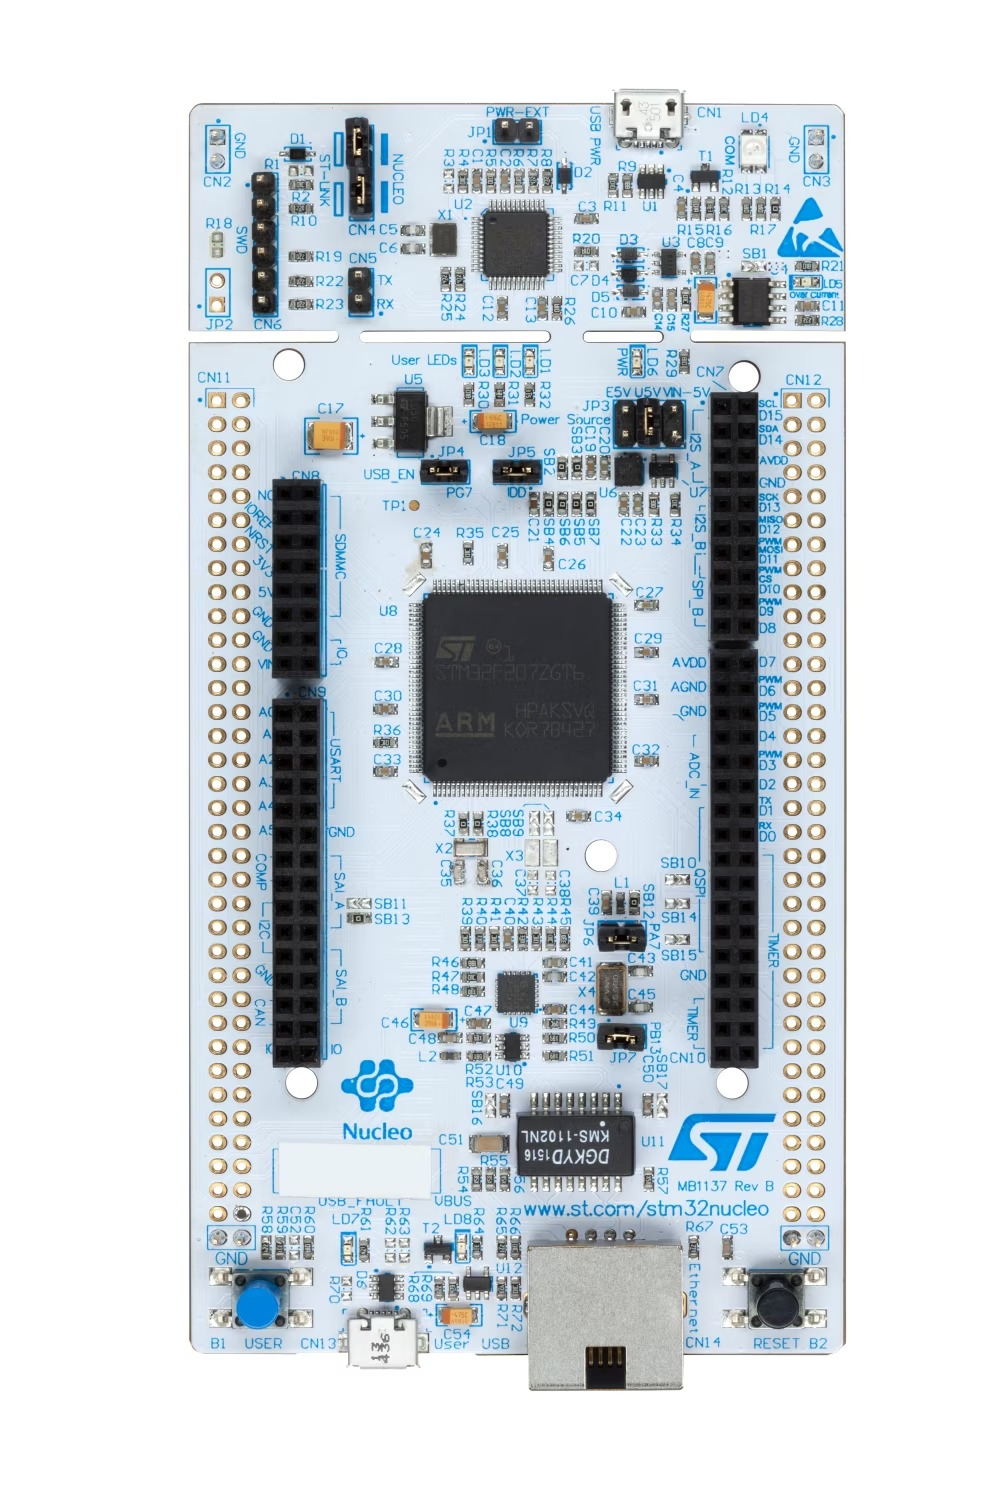
\includegraphics[height=\linewidth, angle=90]{img/nucleo144.jpeg}
    \caption{Placa de desarrollo NUCLEO F429ZI de STMicroelectronics,}
    \label{fig:nucleo144}
\end{figure}



La NUCLEO F429ZI se caracteriza por su gran versatilidad y un conjunto de características técnicas que la hacen adecuada para proyectos que requieren un rendimiento alto y conectividad avanzada. Entre sus especificaciones más destacadas se incluyen:

\begin{itemize}
    \item \textbf{Microcontrolador}: está equipada con un microcontrolador basado en la arquitectura ARM Cortex-M que ofrece un excelente rendimiento junto con una amplia gama de interfaces de conectividad y capacidades avanzadas de procesamiento en tiempo real. La NUCLEO F429ZI incluye el microcontrolador STM32F429ZI \cite{stm32f429zi} tiene un núcleo ARM Cortex-M4 que corre ST-LINK/V2-1a 180 MHz con unidad de punto flotante (FPU), memoria flash de 2 MB y RAM de 256 KB. 

    \item \textbf{Conectividad}: dispone de múltiples interfaces de comunicación, como UART, I2C, SPI, USB, Ethernet y CAN, lo que la convierte en una opción idónea para sistemas que requieren interconexión de múltiples dispositivos y la transmisión de datos en tiempo real.

    \item \textbf{Pines}: incluye un conector de 144 pines, lo que ofrece una gran cantidad de líneas de entrada/salida (GPIO) para controlar y conectar diversos módulos y periféricos. Además, esto permite acceso a todos los pines del microcontrolador lo que permite mayor flexibilidad para la asignación de sus funciones.

    \item \textbf{Programación integrada y \textit{debugging}}: incorpora una interfaz ST-LINK/V2-1 que permite la programación y depuración del microcontrolador sin necesidad de hardware adicional \cite{st_link}. Esto simplifica el desarrollo y facilita la identificación y corrección de errores durante las pruebas del sistema.

    \item \textbf{Alimentación}: puede ser alimentada tanto por USB como por una fuente externa de 5 V o 3,3 V, lo que la hace adaptable a diferentes entornos operativos.
\end{itemize}

Una de las grandes ventajas de la NUCLEO F429ZI es la posibilidad de desarrollar firmware utilizando herramientas muy potentes como STM32CubeIDE \cite{stCubeIde}, que proporciona un entorno de desarrollo completo y gratuito. Mediante una interfaz gráfica, se puede configurar la función de cada uno de los pines, nombrarlos y asegurarse de que no haya superposiciones de definiciones o protocolos de comunicación definidos sin los pines necesarios para que funcione. También facilita la configuración de un sistema operativo en tiempo real, permitiendo la declaración de las distintas tareas y mecanismos de sincronización. Además, el uso de bibliotecas como STM32CubeMX \cite{stCubeMx} facilita la configuración de los periféricos del microcontrolador y la generación de código, reduciendo el tiempo de desarrollo y minimizando la posibilidad de errores. 



\subsubsection{ESP32 Devkit-C}

 El ESP32 Devkit-C es una placa de desarrollo compacta y versátil basada en el microcontrolador ESP32 de Espressif Systems, una solución popular en el ámbito de los sistemas embebidos y aplicaciones IoT \cite{esp32}. Este módulo está diseñado para ofrecer una plataforma accesible para el desarrollo de aplicaciones que requieren conectividad Wi-Fi \cite{ieee_802.11} y Bluetooth \cite{bluetooth}, así como capacidades de procesamiento avanzadas. En la figura \ref{fig:esp32}
 se puede visualizar el módulo ESP32 Devkit-C. \\

 
\begin{figure}[H]
    \centering
    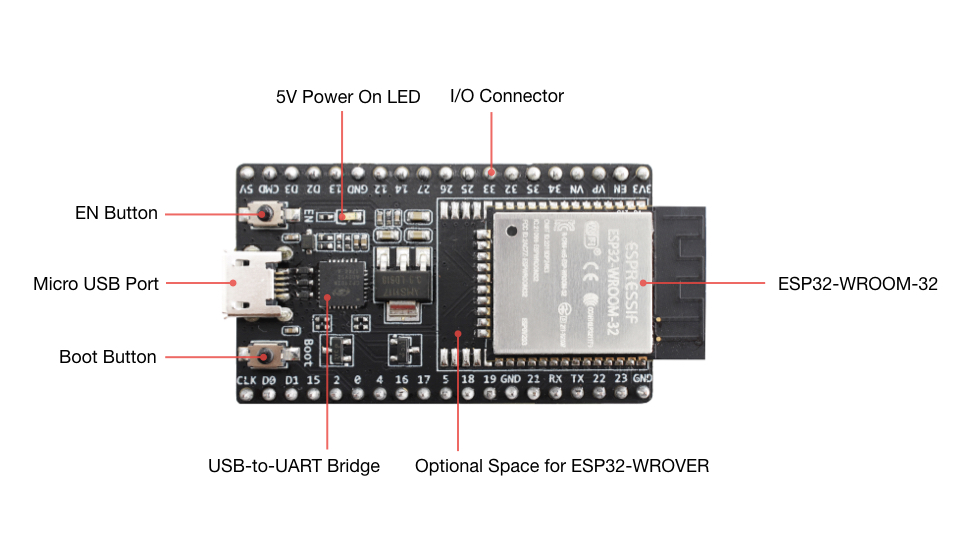
\includegraphics[width=\linewidth]{img/esp32.jpg}
    \caption{Placa de desarrollo ESP32 Devkit-C}
    \label{fig:esp32}
\end{figure}

 
Algunas de las características principales del ESP32 son las siguientes:
\begin{itemize}
    \item \textbf{Microcontrolador dual-core}: Cuenta con un procesador dual-core Xtensa LX6 que opera a una velocidad de hasta 240 MHz. Esta arquitectura multiprocesador permite ejecutar tareas paralelas, lo que resulta ventajoso en aplicaciones donde es necesario manejar múltiples procesos simultáneamente, como la gestión de comunicaciones y control de dispositivos.
    \item \textbf{Conectividad inalámbrica}: Uno de los aspectos más destacados del ESP32 es su capacidad de conectividad inalámbrica:
        \begin{itemize}
            \item \textbf{Wi-Fi 802.11 b/g/n}: Incluye un módulo Wi-FI integrado que permite conectarse a redes inalámbricas, ya sea como cliente o como punto de acceso.
            \item \textbf{Bluetooth 4.2 (BLE y clásico)}: Soporta Bluetooth de baja energía (BLE) y Bluetooth clásico, lo que facilita la comunicación con una amplia variedad de dispositivos, desde teléfonos móviles hasta sensores y actuadores.
        \end{itemize}
    \item \textbf{Amplia gama de interfaces de comunicación}: Ofrece varias interfaces periféricas, lo que lo hace adecuado para interactuar con otros dispositivos y sensores (UART, SPI, I2C, CAN, PWM, ADC y DAC).
    \item \textbf{Memoria}: Incluye 520 KB de SRAM y hasta 16 MB de flash externa, lo que le permite ejecutar aplicaciones complejas y almacenar datos de manera eficiente. Esta combinación de memoria es adecuada para gestionar tanto tareas de conectividad como de procesamiento en tiempo real.
    \item \textbf{Bajo consumo}: Gracias a su arquitectura optimizada para el ahorro de energía, el ESP32 ofrece múltiples modos de bajo consumo, como el modo de suspensión profunda. Esto es especialmente útil en aplicaciones IoT donde la eficiencia energética es crucial y los dispositivos deben funcionar durante largos períodos con baterías limitadas.
    \item \textbf{Capacidades de seguridad}: Está equipado con una serie de características de seguridad integradas, como encriptación de hardware (AES, RSA), arranque seguro y protección de memoria, lo que lo hace adecuado para aplicaciones donde la integridad y confidencialidad de los datos son esenciales.
\end{itemize}


El ESP32 es compatible con una amplia variedad de entornos de desarrollo, entre ellos Arduino IDE \cite{arduino_ide}, Espressif IoT Development Framework (ESP-IDF) \cite{esp_ids} o PlatformIO \cite{platformio}. 
Estas herramientas permiten a los desarrolladores adaptar el entorno de trabajo a sus necesidades específicas. El uso de estos entornos no solo mejora la productividad, sino que también ofrece ventajas clave como facilidad para el desarrollo, una amplia comunidad de soporte, y la capacidad de escalar los proyectos de prototipos a soluciones más avanzadas y robustas.


\subsubsection{Módulo GPS GY-NEO6MV2}

El módulo GPS GY-NEO6MV2 es un receptor GPS de alta precisión que permite obtener datos de ubicación geográfica a través del sistema de posicionamiento global \cite{gy-neo6}. Es ampliamente utilizado en aplicaciones de navegación y rastreo en sistemas embebidos gracias a su bajo consumo de energía y facilidad de integración.\\

Este módulo está basado en el chip NEO-6M de U-blox \cite{neo6}, que proporciona una alta sensibilidad de recepción, incluso en entornos con señal débil. Tiene un conector para antena UFL y es capaz de obtener información como coordenadas geográficas (latitud, longitud), altitud, velocidad y tiempo de posicionamiento, lo que lo hace adecuado para una amplia gama de aplicaciones. En la figura \ref{fig:gps_module} se visualiza el módulo descripto. \\


\begin{figure}[H]
    \centering
    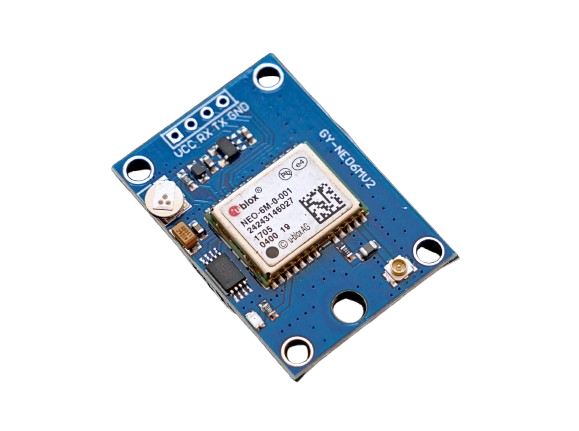
\includegraphics[scale = 0.6]{img/gps_module.png}
    \caption{Módulo GPS GY-NEO6MV2}
    \label{fig:gps_module}
\end{figure}


Algunas de sus características principales son:
\begin{itemize}
    \item Conexión UART para la comunicación con otros dispositivos, facilitando su integración con microcontroladores.
    \item Alta sensibilidad y rápido tiempo de adquisición, incluso en condiciones de baja señal.
    \item Almacenamiento de configuración mediante una memoria EEPROM interna, lo que permite guardar parámetros de configuración para su uso posterior sin necesidad de reconfigurar el módulo al encenderlo.
\end{itemize}



Gracias a su tamaño compacto y bajo consumo, el GY-NEO6MV2 es ideal para sistemas que requieren monitoreo de posición en tiempo real con un costo y consumo energético reducidos.
\subsubsection{Tarjetas SD}

Las tarjetas SD (\textit{Secure Digital}) son dispositivos de almacenamiento de datos que han ganado popularidad debido a su tamaño compacto, capacidad de almacenamiento y facilidad de uso. Son ampliamente utilizadas en diversas aplicaciones, desde cámaras digitales hasta sistemas embebidos, gracias a su versatilidad y eficiencia. En la figura \ref{fig:sd_card} se visualiza una tarjeta SD.\\


\begin{figure}[H]
    \centering
    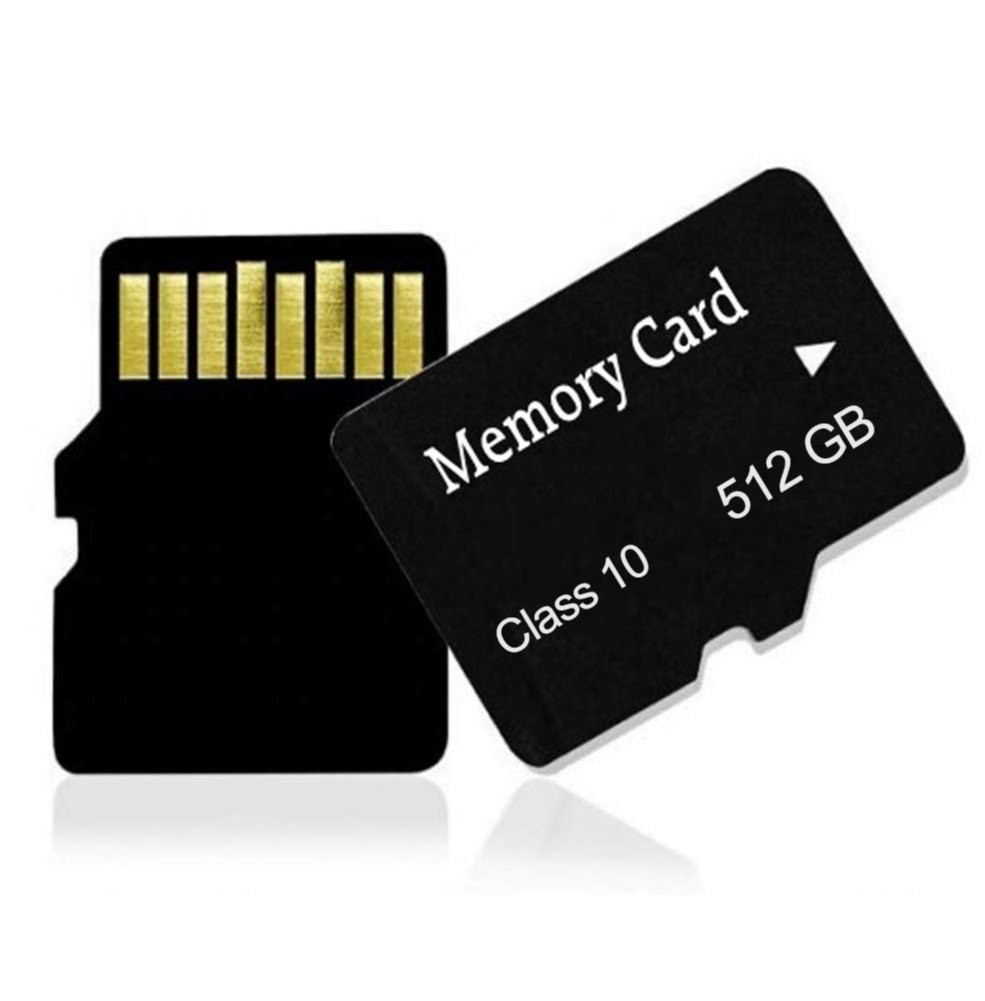
\includegraphics[scale = 0.2]{img/sd_card.jpg}
    \caption{Tarjeta SD}
    \label{fig:sd_card}
\end{figure}



Las tarjetas SD cuentan con las principales características: 
\begin{itemize}
    \item \textbf{Capacidad de almacenamiento}: Las tarjetas SD están disponibles en varias capacidades, que varían desde unos pocos megabytes hasta varios terabytes. Esto permite a los usuarios elegir la tarjeta adecuada según sus necesidades específicas de almacenamiento.
    \item \textbf{Velocidades de transferencia}: Existen diferentes clases de tarjetas SD, como Clase 2, 4, 6, 10, y UHS-I y UHS-II, que determinan la velocidad mínima de lectura y escritura. Las tarjetas de clase más alta son ideales para aplicaciones que requieren una rápida transferencia de datos, como la grabación de video en alta definición.
    \item \textbf{Interfaz de comunicación}: Las tarjetas SD utilizan una interfaz estándar que permite la conexión con dispositivos a través de protocolos como SPI (\textit{Serial Peripheral Interface}) o SDIO (\textit{Secure Digital Input Output}). Esto facilita su integración en una variedad de sistemas.
    \item \textbf{Durabilidad y fiabilidad}: Muchas tarjetas SD están diseñadas para resistir condiciones adversas, como temperaturas extremas, golpes y vibraciones. Esto las hace adecuadas para su uso en entornos donde la robustez es fundamental.
    \item \textbf{Facilidad de uso}: La implementación de tarjetas SD es sencilla, ya que muchos dispositivos y plataformas de desarrollo ofrecen bibliotecas y herramientas que facilitan la lectura y escritura de datos en estas tarjetas.
\end{itemize}



En los sistemas embebidos las tarjetas SD se colocan sobre un zócalo que permite removerlas para luego insertar la tarjeta SD en una PC y descargar los datos, formatearla o repararla. También existen módulos para Arduino que permiten integrar una tarjeta SD al proyecto en etapas tempranas antes de fabricar un PCB propio y soldar un zócalo. Esto facilita mucho el mantenimiento y el desarrollo de sistemas que contienen almacenamiento de memoria en tarjetas SD. Las tarjetas SD se han convertido en una solución de almacenamiento clave en muchos dispositivos electrónicos, ofreciendo una combinación de flexibilidad, capacidad y rendimiento que se adapta a una amplia gama de aplicaciones.
\subsection{Protocolos de comunicación}
\subsubsection{MQQT}        

MQTT (\textit{Message Queuing Telemetry Transport}) es un protocolo de comunicación ligero diseñado específicamente para entornos con limitaciones de ancho de banda, latencia o recursos, lo que lo hace ideal para aplicaciones de IoT. Desarrollado por IBM en 1999 \cite{mqtt_ibm}, MQTT sigue el modelo \textit{publish/subscribe}, lo que permite la transmisión eficiente de mensajes entre dispositivos conectados sin necesidad de una conexión constante y directa entre ellos. \\


El protocolo MQTT utiliza una arquitectura basada en los siguientes componentes clave que se pueden visualizar su interacción en la figura \ref{fig:mqtt}:

\begin{itemize}
    \item \textbf{\textit{Broker}}: es el servidor central que gestiona la recepción y distribución de los mensajes. El \textit{broker} es responsable de recibir los mensajes de los \textit{publishers} y reenviarlos a los \textit{subscribers} que se hayan suscrito al tema correspondiente.

    \item \textbf{\textit{Publisher}}: es el dispositivo o cliente que envía un mensaje a un tema específico, sin necesidad de conocer a los destinatarios. Solo necesita enviar el mensaje al \textit{broker}.

    \item \textbf{\textit{Subscriber}}: es el dispositivo o cliente que recibe los mensajes de un tema al cual se ha suscrito previamente. El suscriptor se comunica únicamente con el \textit{broker} y no directamente con los publicadores.

    \item  \textbf{\textit{Topics}}: los \textit{topics} o temas son etiquetas jerárquicas utilizadas para categorizar los mensajes en MQTT. Cuando un publicador envía un mensaje, lo asocia con un tema específico. Los suscriptores que se suscriben a ese tema recibirán los mensajes. La flexibilidad de los \textit{topics} permite organizar la información de manera eficiente y estructurada.
\end{itemize}

\begin{figure}[H]
    \centering
    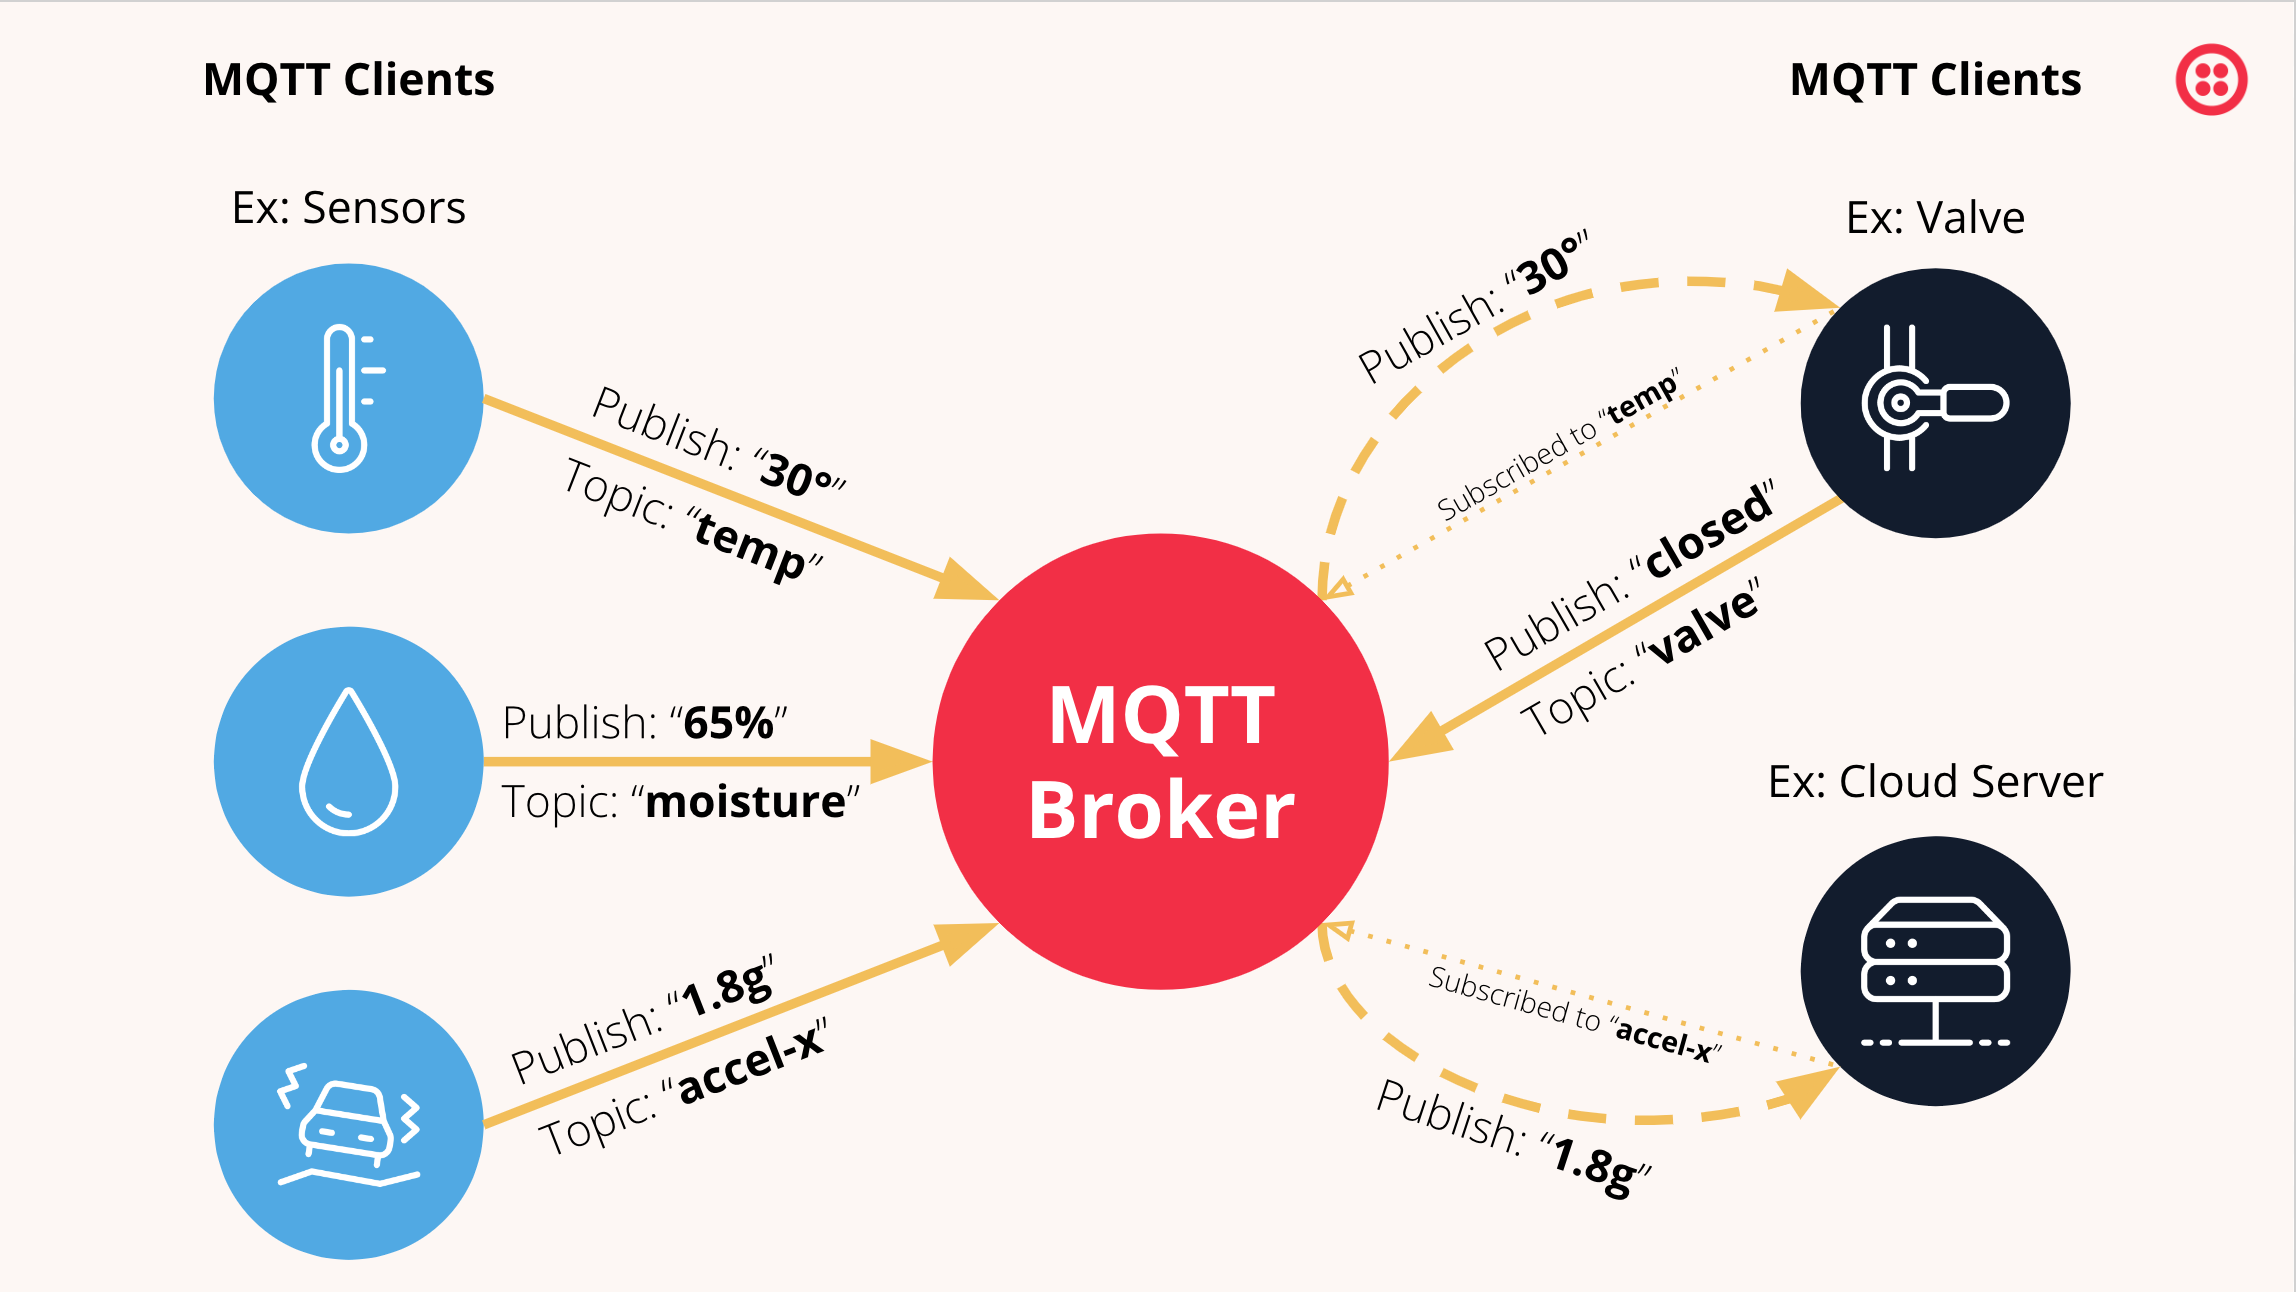
\includegraphics[width = 0.8 \linewidth]{img/mqtt.png}
    \caption{Diagrama de conexión MQTT de ejemplo \cite{mqtt_img}}
    \label{fig:mqtt}
\end{figure}



Las principales ventajas del protocolo MQTT se pueden resumir en:

\begin{itemize}
    \item \textbf{Ligereza}: MQTT está diseñado para ser extremadamente eficiente en cuanto a recursos, lo que lo hace ideal para dispositivos con capacidades limitadas, como sensores o microcontroladores.
    \item \textbf{Minimización del consumo de energía}: al ser un protocolo que no requiere mantener conexiones activas todo el tiempo, los dispositivos pueden ahorrar energía, lo que es fundamental en aplicaciones IoT.
    \item \textbf{Comunicación asíncrona}: gracias a su modelo de publicación y suscripción, los dispositivos no necesitan estar conectados constantemente. El \textit{broker} gestiona las comunicaciones y distribuye los mensajes a los suscriptores según sea necesario.
\end{itemize}



MQTT es ampliamente utilizado en aplicaciones IoT, como monitoreo remoto, automatización industrial, gestión de energía y sistemas embebidos. También se ha implementado en sistemas de emergencia, control de dispositivos y telemetría, donde la eficiencia y la fiabilidad son esenciales.
\subsubsection{Wi-Fi}

Wi-Fi (\textit{Wireless Fidelity}) es un conjunto de tecnologías que permiten la comunicación inalámbrica entre dispositivos electrónicos utilizando ondas electromagnéticas. Es uno de los protocolos de comunicación más comunes en redes locales (WLAN) y se basa en la familia de estándares IEEE 802.11 \cite{ieee_802.11}, desarrollados y mantenidos por el Instituto de Ingenieros Eléctricos y Electrónicos (IEEE). Wi-Fi es ampliamente utilizado en aplicaciones que requieren conectividad a internet o comunicación local sin cables, lo que lo convierte en una opción clave en proyectos de IoT y sistemas embebidos. \\


Wi-Fi opera en bandas de frecuencia de 2.4 GHz y 5 GHz, y permite a los dispositivos conectarse a una red a través de un punto de acceso (\textit{Access Point}) o funcionar en un modo de conexión directa \textit{peer-to-peer} (ad-hoc). En la figura \ref{fig:wifi} se visualizan los dos tipos de conexiones mencionadas. En un entorno típico, un \textit{router} actúa como el punto de acceso central, al cual se conectan varios dispositivos para intercambiar datos entre sí y acceder a internet. \\ 

\begin{figure}[H]
    \centering
    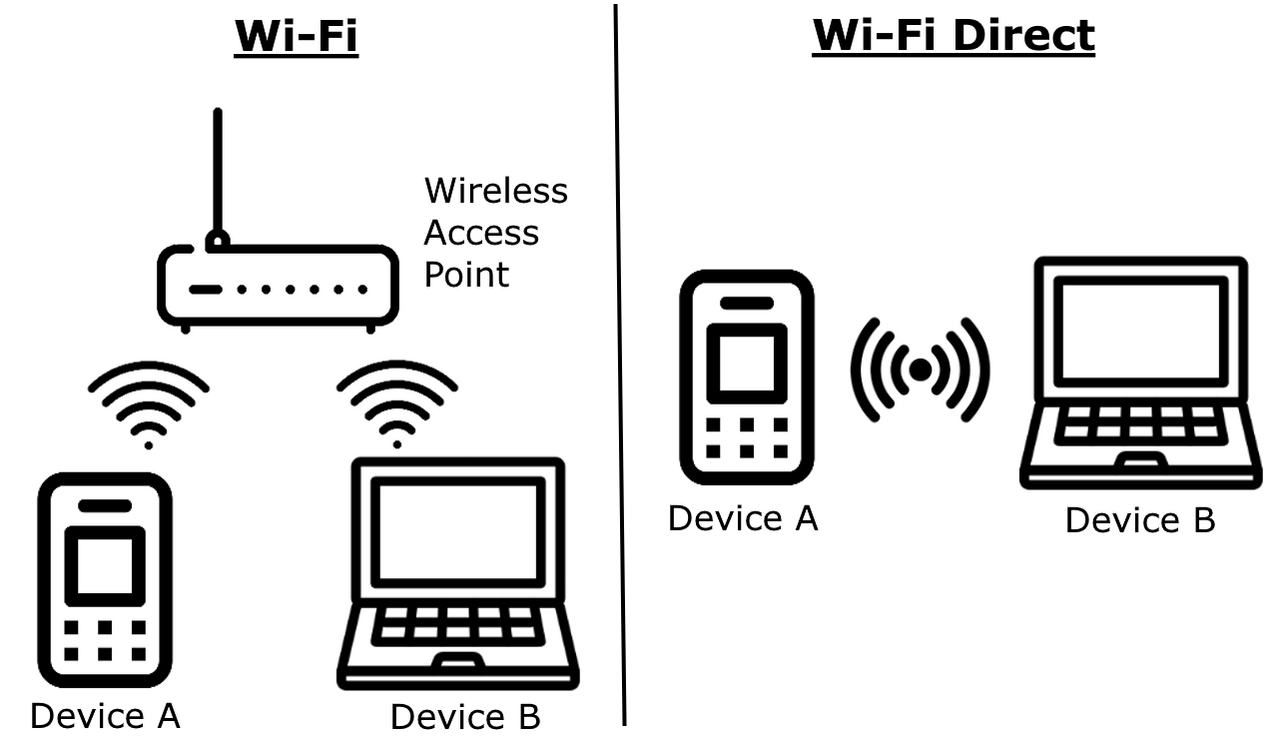
\includegraphics[width = 0.7 \linewidth]{img/wifi.png}
    \caption{Modos de conexión Wi-Fi \cite{wifi_img}}
    \label{fig:wifi}
\end{figure}


Las principales características de Wi-Fi son las siguientes:

\begin{itemize}
    \item \textbf{Alcance}: Ofrece un rango de cobertura considerable, que generalmente varía entre 20 a 50 metros en interiores y hasta 100 metros en exteriores, dependiendo de las condiciones de señal y el entorno.
    
    \item \textbf{Velocidad}: Permite transmitir datos a distintas velocidades según la señal y las condiciones de la red, ofreciendo un rendimiento adecuado para la mayoría de las aplicaciones cotidianas.
    
    \item \textbf{Seguridad}: Incorpora varios protocolos de seguridad, como WEP, WPA y WPA2 \cite{wifi_security}, que aseguran la comunicación cifrada entre dispositivos y protegen las redes inalámbricas de accesos no autorizados.
    
    \item \textbf{Compatibilidad}: Es retrocompatible, lo que significa que los dispositivos más antiguos que soportan versiones previas del estándar, como 802.11a, b, g o n, pueden seguir conectándose a redes más modernas, aunque con limitaciones en velocidad y funcionalidad.
    
   
\end{itemize}






El protocolo Wi-Fi cuenta con algunas limitaciones como su consumo de energía; que suele ser mayor comparado con otros protocolos con el Bluetooth, o la congestión y colisiones que pueden ocurrir en entornos densos con muchos dispositivos conectados; esto puede generar interferencia y degradación en el rendimiento de las conexiones. \\

Sin embargo, el Wi-FI se popularizó cada vez más debido las siguientes ventajas que genera:

\begin{itemize}
    
    \item \textbf{Flexibilidad}: Elimina la necesidad de cables, lo que facilita la instalación y operación en entornos móviles o de difícil acceso. Esto es especialmente útil en redes IoT donde se requiere la conectividad de múltiples dispositivos dispersos.

    
    \item \textbf{Conectividad global}: La mayoría de los dispositivos modernos, desde teléfonos móviles hasta microcontroladores y computadoras, tienen Wi-Fi integrado, lo que permite la interoperabilidad entre diferentes plataformas y tecnologías.

    \item \textbf{Alta velocidad de transmisión}: Es adecuado tanto para aplicaciones que requieren grandes volúmenes de datos, como la transmisión de video en tiempo real, como para aquellas que necesitan una transferencia rápida, como la telemetría o la comunicación de sensores.
\end{itemize}


Wi-Fi es el protocolo preferido para aplicaciones que requieren transferencias rápidas y confiables de datos, como transmisión de video, comunicación entre dispositivos móviles, automatización del hogar y acceso a internet en redes locales. También es fundamental en muchas aplicaciones de IoT que requieren conectividad en tiempo real y de alto ancho de banda.
\subsubsection{GPS}

El GPS (\textit{Global Positioning System}) es una tecnología de navegación por satélite que permite determinar la ubicación geográfica exacta de un objeto o dispositivo en cualquier parte del mundo. El sistema fue desarrollado por el Departamento de Defensa de los Estados Unidos \cite{gps} y está compuesto por una red de satélites que transmiten señales de tiempo y posición generalmente en la banda de frecuencia L1 1.57542 GHz para usos civiles. Los dispositivos con receptores GPS pueden calcular su posición en la Tierra midiendo el tiempo que tarda la señal en viajar desde los satélites. \\


El GPS utiliza una técnica llamada trilateración para determinar la posición de un dispositivo. Para calcular su ubicación, el receptor GPS necesita recibir señales de al menos cuatro satélites. A partir de estas señales, el receptor puede calcular la distancia a cada satélite y determinar con precisión su posición en coordenadas geográficas (latitud, longitud y altitud). El GPS utiliza cuatro satélites en lugar de tres para calcular no solo la ubicación en tres dimensiones, sino también para corregir errores en el reloj del receptor y obtener mayor precisión. En la figura \ref{fig:gps} se visualiza cómo un receptor recibe señales de 4 satélites lo que le permite determinar su ubicación. \\

\begin{figure}[H]
    \centering
    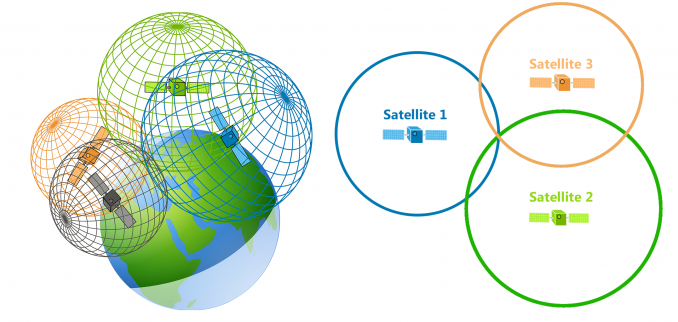
\includegraphics[width = 0.7 \linewidth]{img/gps.png}
    \caption{Trilateración utilizada en GPS \cite{gps_img}}
    \label{fig:gps}
\end{figure}



En los sistemas embebidos, los módulos GPS se utilizan ampliamente para aplicaciones que requieren posicionamiento y geolocalización. Estos módulos son pequeños, de bajo consumo de energía y fáciles de integrar en una amplia variedad de dispositivos y proyectos. Algunas aplicaciones comunes en sistemas embebidos incluyen:

\begin{itemize}
    \item \textbf{Monitoreo de vehículos}: el GPS es utilizado para rastrear vehículos en tiempo real, facilitando sistemas de logística, transporte público y servicios de emergencia.

    \item \textbf{Agricultura de precisión}: equipos agrícolas con GPS pueden optimizar la siembra, el riego y la cosecha mediante la geolocalización precisa.

    \item \textbf{Dispositivos IoT}: muchos dispositivos conectados a Internet, como drones, sensores o sistemas de automatización, utilizan GPS para la recolección de datos de ubicación.

    \item \textbf{Navegación y mapeo}: desde sistemas de navegación portátiles hasta drones y robots autónomos, el GPS permite trazar rutas y moverse eficientemente por entornos dinámicos.
\end{itemize}


La utilización de GPS provee una alta precisión que varía desde los pocos metros hasta los centímetros (dependiendo de las condiciones y el equipo). También tiene la ventaja de contar con una cobertura global lo que permite una solución de geolocalización sin necesidad de infraestructura adicional. Además, los módulos GPS para sistemas embebidos están diseñados para ser eficientes energéticamente, lo que los hace ideales para dispositivos portátiles o alimentados por baterías. \\ 

En resumen, la tecnología GPS ha revolucionado la capacidad de los sistemas embebidos para obtener y procesar datos de ubicación de manera eficiente y precisa. Su integración en dispositivos y aplicaciones es clave para una variedad de sectores, como la logística, la agricultura y el IoT, proporcionando soluciones versátiles y de bajo consumo para necesidades de geolocalización. La combinación de su cobertura global y su capacidad de adaptación lo convierte en una herramienta fundamental en el diseño de sistemas embebidos modernos.
\subsubsection{RS485}

El RS485 es un estándar de comunicación serial que se utiliza ampliamente en aplicaciones industriales y de automatización debido a su robustez y fiabilidad \cite{rs485}. A diferencia de otros protocolos de comunicación como UART o SPI, el RS485 permite la comunicación de múltiples dispositivos en un mismo bus de datos sin necesidad de agregar una línea de selección por cada dispositivo, lo que lo hace ideal para redes en las que se requiere que varios dispositivos compartan una única línea de comunicación. En la figura \ref{fig:res485} se visualiza un bus de RS485 con varios dispositivos conectados en modo \textit{half-duplex} (los dispositivos pueden enviar o recibir, pero no ambas cosas al mismo tiempo). \\ 

\begin{figure}[H]
    \centering
    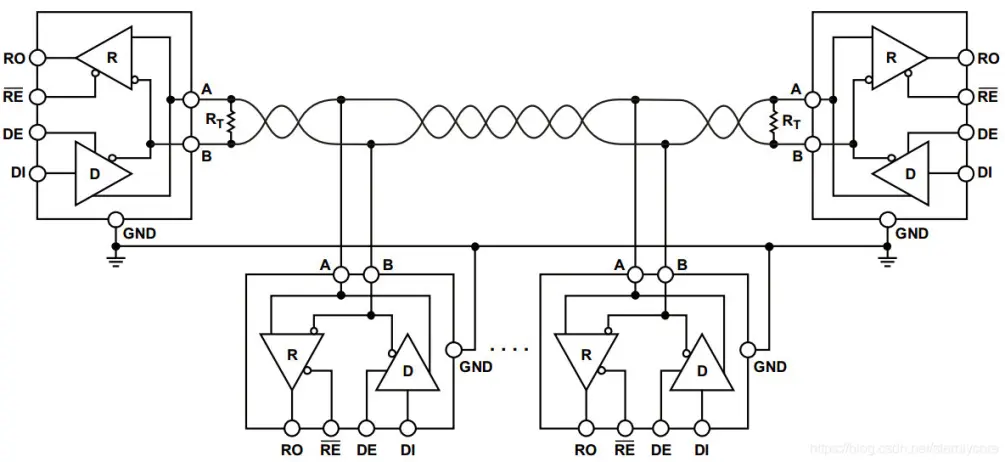
\includegraphics[width =  \linewidth]{img/rs485.png}
    \caption{Bus RS485 en modo \textit{half-duplex}}
    \label{fig:res485}
\end{figure}

Alguna de las características principales del protocolo RS485 son las siguientes: 

\begin{itemize}
    \item \textbf{Comunicación diferencial}: RS485 utiliza dos líneas para la transmisión de datos (A y B), lo que le permite operar bajo el principio de comunicación diferencial. Esto significa que el valor lógico de los datos se determina por la diferencia de tensión entre las dos líneas, lo que mejora la inmunidad al ruido y permite transmitir datos a largas distancias sin degradación de la señal.

    \item \textbf{Distancia y velocidad}: Puede transmitir datos a distancias de hasta 1200 metros, dependiendo de la velocidad de comunicación. A velocidades bajas (por ejemplo, 100 kbps), puede cubrir distancias más largas, mientras que a velocidades más altas (por ejemplo, 10 Mbps), la distancia máxima disminuye.

    \item \textbf{Topología multipunto}: Una de las ventajas más notables de RS485 es su capacidad para soportar comunicación multipunto, permitiendo que hasta 32 dispositivos se conecten en el mismo bus sin necesidad de repetidores. Esto es muy útil en entornos donde varios dispositivos necesitan intercambiar información, como en redes de sensores o controladores.

    \item \textbf{Modo \textit{half-duplex} y \textit{full-duplex}}: RS485 se puede configurar tanto en modo half-duplex como en modo full-duplex (utilizando dos pares de cables para permitir la transmisión y recepción simultánea).

    \item \textbf{Robustez}: Debido a su capacidad de resistir interferencias electromagnéticas y operar en entornos industriales hostiles, RS485 es ampliamente utilizado en aplicaciones donde la fiabilidad y la estabilidad de la comunicación son cruciales.

\end{itemize}

La flexibilidad en la topología de red es una de las ventajas significativas del protocolo RS485. A diferencia de otros estándares seriales como RS232, que se limitan a la comunicación punto a punto, el RS485 permite configuraciones de red en bus o \textit{multidrop}. Esto lo convierte en una opción ideal para sistemas distribuidos donde varios nodos necesitan intercambiar datos de manera eficiente. Además, en aplicaciones que requieren una mayor distancia o más dispositivos en el bus, se pueden utilizar repetidores o extensores para ampliar el alcance y la capacidad de la red sin comprometer la calidad de la señal. Esta versatilidad, junto con su capacidad para operar en entornos hostiles, ha hecho que RS485 sea una solución de comunicación robusta y ampliamente adoptada en el ámbito industrial y de control.
\subsection{Sistema operativo de tiempo real}

Un sistema operativo en tiempo real (RTOS por sus siglas en inglés) es un tipo de sistema operativo diseñado para gestionar tareas de manera determinista, garantizando que ciertas operaciones se completen dentro de plazos definidos \cite{rtos}. A diferencia de los sistemas operativos convencionales, donde la prioridad de las tareas puede variar según la carga del sistema, un RTOS garantiza que las tareas críticas se ejecuten en tiempo y forma según su prioridad. \\

Los RTOS son fundamentales en aplicaciones embebidas donde es crucial que las respuestas a eventos externos, como la activación de un sensor o una interrupción, se produzcan dentro de tiempos predeterminados. Estos sistemas son ampliamente utilizados en sectores como el automotriz, la aviación, las telecomunicaciones, y los sistemas médicos. \\

Algunas características clave de los RTOS incluyen:

\begin{itemize}
    \item \textbf{Determinismo}: El comportamiento predecible en cuanto a la ejecución de tareas es esencial. Un RTOS asegura que las tareas se ejecuten de acuerdo con una planificación estricta, cumpliendo con los plazos impuestos por el sistema.

    \item \textbf{Multitarea}: Un RTOS es capaz de manejar múltiples tareas concurrentemente, priorizando aquellas que son más críticas para el sistema.

    \item \textbf{Gestión de interrupciones}: La rápida respuesta a interrupciones de hardware es vital en un RTOS. Estos sistemas permiten que las tareas de mayor prioridad respondan rápidamente a eventos externos, sin demoras significativas.

    \item \textbf{Uso eficiente de recursos}: Dado que los RTOS suelen implementarse en sistemas embebidos con recursos limitados, están optimizados para ser ligeros y eficientes en términos de memoria y procesamiento.

\end{itemize}


En la figura \ref{fig:freertos_tasks} se muestra un ejemplo de un RTOS realizando asignación de tareas con distintas prioridades e interactuando con una interrupción por hardware. 

\begin{figure}[H]
    \centering
    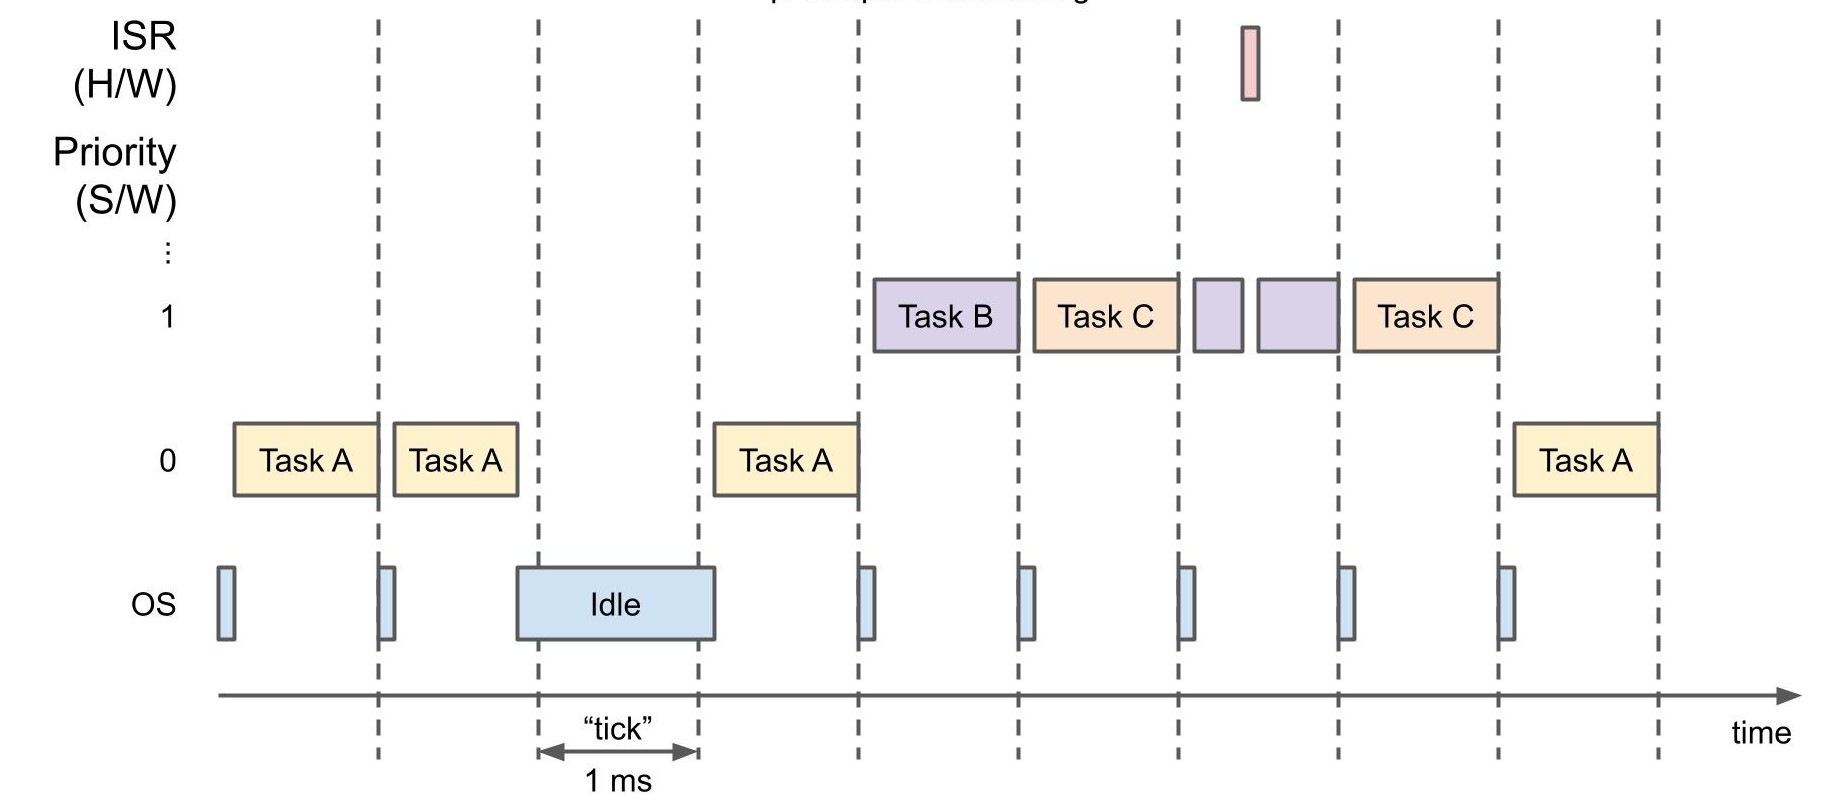
\includegraphics[width = \linewidth]{img/freertos_tasks.jpeg}
    \caption{Asignación de tareas por prioridades en un RTOS}
    \label{fig:freertos_tasks}
\end{figure}





\newpage
\section{Diseño e implementación}
\input{3 - Diseño e implementación/3.1 - Descripción general de la solución}

\subsection{Implementación de hardware}
\subsubsection{Medición de estado de los SIS}

El SAL/T debe interactuar con 5 sistemas instrumentados de seguridad (SIS) que cada uno cuenta con 2 llaves de estado; una para la línea de la señal crítica de corte de tracción (CT) y la otra para la señal crítica de freno de emergencia (FE). Estas llaves van a estar en un estado cerrado cuando el SIS esté funcionando correctamente y no detecte ninguna situación peligrosa en la formación, y se van a abrir para interrumpir la alimentación de las señales críticas ante una falla en el SIS o la detección de alguna condición peligrosa. \\ 

Considerando el diagrama de conexión ya presentado en la figura \ref{fig:señales_criticas}, se puede interpretar que, cuando la llave está cerrada, por definición, la diferencia de tensión entre sus terminales va a ser nula. En cambio, si en toda la línea existe un único interruptor abierto, se espera que toda la tensión de alimentación $V_{ALIM}$ que en el terminal positivo de la llave mientras que en el terminal negativo, debería haber una tensión de tierra, ya que, al abrir el circuito, no va a circular corriente por la línea y la electroválvula no va a agregar ninguna caída de tensión. Por lo tanto, se pueden resumir la diferencia de tensión esperada en los terminales de un SIS en la tabla \ref{tab:switch_state}. 

\begin{table}[htb]
    \begin{tabular}{|c|c|} 
        \hline
        \textbf{Estado de llave} & \textbf{Tensión entre terminales}\\
        \hline
        Cerrada     &     0 V   \\
        \hline
        Abierta     &     $V_{ALIM}$ \\
        \hline
    \end{tabular}
    \label{tab:switch_state}
    \caption{Diferencia de tensión entre los terminales de un SIS}
\end{table}

Los rangos de tensión de alimentación de las baterías de las formaciones consideradas son $ 72 VDC < V_{ALIM} < 110 VDC $. Y considerando que estos buses de mayor tensión pueden no tener una puesta de tensión en común con el SAL/T, se decidió utilizar un circuito de medición diferencial para calcular la tensión entre las terminales de un interruptor independientemente de su tensión contra la tierra del circuito y luego conectar la tensión medida en un conversor analógico digital (ADC) del microcontrolador para poder obtener de manera digital un valor para la tensión. \\ 


Con el objetivo de alterar lo menos posible línea de las señales críticas, se optó por utilizar un amplificador de instrumentación para poder medir la tensión diferencial entre los terminales de las llaves. Este dispositivo permite medir una tensión diferencial rechazando cualquier señal de modo común con una gran impedancia de entrada lo que permite derivar una pequeña corriente de la línea principal sin alterarla. El modelo seleccionado fue el INA823DGKR de Texas Instrument \cite{INA823DGKR}; un amplificador de instrumentación con salide \textit{single-ended} con un rango de ganancia programable de 1 a 1000 con una resistencia externa, con una baja corriente de polarización de entrada de 1.2 nA y permite la alimentación con una fuente dual de $\pm1.1 V$ a $\pm18 V$. Para la aplicación en el SAL/T, se va a utilizar una ganancia de 1 (sin resistencia externa conectada) y se va a alimentar el amplificador con una tensión dual de $\pm5 V$.\\

Para generar la tensión de -5V a partir de la fuente de alimentación de +5V, se utilizó el regulador de tensión ICL7660AIBAZA de Renesas Electronics \cite{ICL7660AIBAZA} diseñado para invertir una tensión de entrada positiva y generar una salida negativa. Este permite la inversión de la tensión de entrada en el rango de 1.5 V a 12 V, tiene un bajo consumo de corriente de 80 $\mu$A, funciona con un oscilador interno a 10KHz que elimina la necesidad de generar una señal de reloj externa y solo requiere dos capacitores externos. El circuito integrado (CI) viene en un encapsulado VSSOP-8 para montaje superficial. En la figura \ref{fig:ICL7660AIBAZA}, se observa la conexión del ICL7660AIBAZA siguiendo las recomendaciones de la hoja de datos para una tensión de entrada de +5V; se utilizaron 2 capacitores electrolíticos de 10 $\mu$F y se obtuvo una tensión de salida de -5V. 

 
\begin{figure}[H]
    \centering
    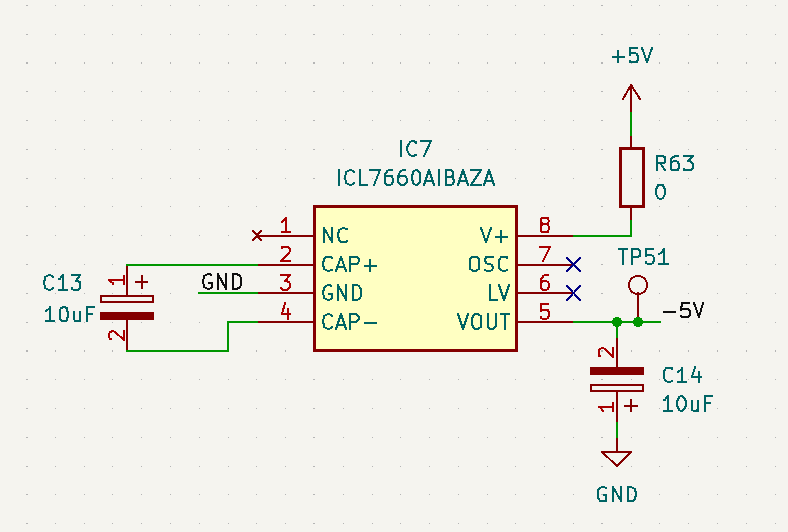
\includegraphics[width = 0.8 \linewidth]{img/ICL7660AIBAZA.png}
    \caption{Esquemático del circuito para generación de tensión de alimentación negativa}
    \label{fig:ICL7660AIBAZA}
\end{figure}


Para poder medir la tensión diferencial en las terminales de las llaves del SIS con el INA823DGKR alimentado con $\pm$5V, es necesario adaptar las tensiones a medir a un rango dentro de los extremos de la alimentación, ya que podría haber una diferencia de hasta 110V sobre esa llave. Para reducir esta tensión diferencial, se implementó una red de resistencias que permitan mantener la diferencia de tensión, pero reducida por un factor seleccionado y utilizando una tierra como referencia para tener las tensiones positivas y negativas a la entrada del amplificador de instrumentación. \\ 

Si bien el rango máximo para las entradas podía ser $\pm$5V, considerando que la ganancia del amplificador es 1 y que la salida va a ingresar a un ADC del microcontrolador que trabaja en un rango de hasta 3V3 de entrada, hay que reducir el rango máximo esperado hasta esa tensión. Por lo tanto, si consideramos 110 V como la máxima tensión diferencial en la llave del SIS, y armando una red de resistencias que parta esta tensión a la mitad colocando una tierra en la mitad del circuito, se debe calcular los valores de las resistencias tal que, en cada entrada del amplificador, haya como máximo una tensión de $\pm$1.65 V, ya que, la salida es \textit{single-ended} y para esos valores máximos usaría el rango completo de 3V3 del ADC. Considerando un divisor resistivo para cada terminal del SIS, que se conecten con una tierra a la mitad, se pueden calcular los valores de las resistencias con las siguientes ecuaciones: 

\begin{equation}
    \frac{V_{max\_ADC}}{2} = \frac{V_{max\_SIS}}{2} \cdot \frac{R2}{R1 + R2}    
\end{equation}

Despejando el divisor resistivo invertido para facilitar la selección de valores de resistencia y utilizando $ V_{max_ADC}=3.3V$  y $V_{max\_SIS} = 110 V$: 

\begin{equation}
    \frac{R1 + R2}{R2}  = \frac{V_{max\_ADC}}{V_{max\_SIS}} = 33.33
\end{equation}

Esto significa que la resistencia R1 tiene que ser, aproximadamente 33.33 veces más grandes que R2. Además, considerando que se busca extraer la menor corriente posible de la línea de los SIS, se van a utilizar valores de resistencia muy altos así como también el amplificador cuenta con una impedancia de entrada muy alta. Con estos cálculos realizados, se seleccionaron los valores de R1=1 M$\Omega$ y R2=30 K$\Omega$ lo que genera un divisor resistivo de 34.33 veces la tensión original; esto permite estar darle un poco de margen al rango máximo calculado. \\



Con las distintas partes del circuito resueltas, en la figura \ref{fig:sis_medicion} se muestra un esquemático del circuito de medición de los SIS con los elementos explicados donde también se agregan 2 capacitores de desacople en la alimentación del amplificador para filtrar cualquier ruido que pueda venir en la línea. 



\begin{figure}[H]
    \centering
    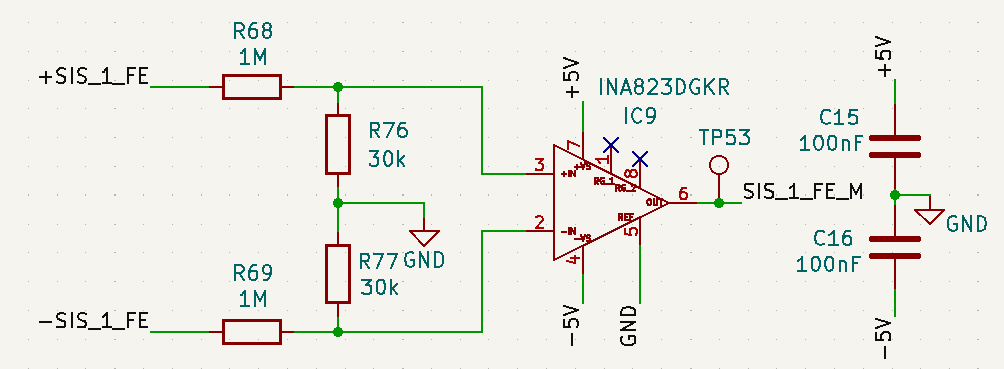
\includegraphics[width = \linewidth]{img/sis_medicion.png}
    \caption{Esquemático del circuito de medición de los SIS}
    \label{fig:sis_medicion}
\end{figure}



\subsubsection{Aislamiento de los SIS}




La interacción con los sistemas instrumentados de seguridad se produce en la medición del estado impuesto por los propios SIS, pero también en una imposición de estado por parte del SAL/T. La llave interruptora de los SIS se abre ante una falla o detección de condición insegura en ese SIS. Sin embargo, el propósito del SAL/T es permitir el movimiento de la formación de una manera segura ante una activación de las interrupciones de los SIS. En el caso de ingresar al modo aislado limitado (MAL), el sistema va a utilizar las mediciones de estado de cada uno de los SIS y aislar el que esté interrumpiendo la línea; de esta manera, la línea mantiene la continuidad, y el resto de los SIS siguen teniendo la capacidad de interrumpir las señales críticas. Además, cuando se ingresa en modo aislado total (MAT) o en modo intermitente por comando remoto, o en modo parada total o en modo coche deriva, el SAL/T va a interrumpir las líneas de las señales críticas dejando sin efecto el estado de los SIS. \\    

Para realizar el aislamiento de un SIS, se conectaron las mismas terminales donde se mide el estado del SIS a un relé. Su estado normal es abierto, por lo que no afecta el estado del SIS. Sin embargo, cuando se activa la señal de control del relé por algunos de los motivos mencionados anteriormente, se conectan las señales positiva y negativa de la llave del SIS, forzando un estado de continuidad en la línea. \\ 

Para el relé de aislamiento, se eligió el modelo JW2SN-DC5V de Panasonic Industrial Devices \cite{JW2SN-DC5V}. Este es un relé de potencia que se activa con 5 V en las entradas de control y que cuenta con un arreglo de contacto de 2 salidas tipo C conocido como DPDT (\textit{double-pole double-throw}). En condiciones normales, tiene un consumo de 106 mA al activarse, ya que la resistencia de la bobina interna es de 47 $\Omega$. \\

Se eligió este modelo porque funciona como exacto reemplazo de un relé de seguridad de las mismas características de encapsulamiento y contactos como el V23047A1005A501 de TE Connectivity \cite{V23047A1005A501}. Estos relés de seguridad también son DPDT y activan con 5 VDC. Los relés de seguridad o también conocidos como relé de contactos guiado forzado tienen una configuración y técnica constructiva que cumplen con la norma EN 61810-3 \cite{norma_61810}. Estos relés tienen al menos un par de contactos normal cerrado y otro par normal abierto que están vinculadas de manera mecánica lo que hace imposible que ambos estén en contacto simultáneamente; incluso en caso de falla. En la figura \ref{fig:rele_seguridad} se observa el funcionamiento de un relé de seguridad. Este tipo de relé es recomendado para aplicaciones en sistemas críticos porque permite utilizar el contacto primario como actuador, mientras que el contacto secundario se puede utilizar para monitorear su correcto funcionamiento. \\



\begin{figure}[H]
    \centering
    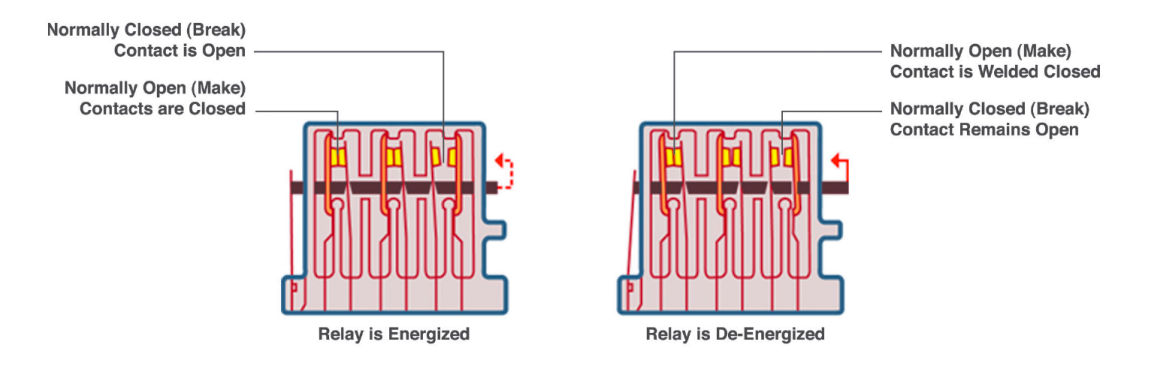
\includegraphics[width = \linewidth]{img/rele_seguridad.png}
    \caption{Funcionamiento de un relé de seguridad \cite{rele_img}}
    \label{fig:rele_seguridad}
\end{figure}


El modelo utilizado en este prototipo, el JW2SN-DC5V es un relé de uso general, pero se optó por reemplazar el relé de seguridad por este modelo de uso general por la gran diferencia que hay en los costos entre los modelos y considerando que el sistema total hace uso de más de 20 relés. \\

Una de las salidas del JW2SN-DC5V se va a utilizar como actuador y la otra para medir el correcto funcionamiento del relé. Para eso, las salidas del contacto secundario van a estar conectadas una a tierra y la otra a una tensión de 3V3 y la llave secundaria que conmuta va a estar conectada a una entrada digital del MCU para medir el estado de esa llave. A partir de este estado, el sistema puede determinar luego si hay un estado de error y debe tomar medidas para llevar el sistema a un estado seguro. \\


Para poder energizar el relé con una corriente de poco más de 100mA es necesario utilizar un driver de potencia, ya que la corriente es demasiada alta para drivear directamente desde el MCU además de que la tensión de activación es de 5V y el MCU tiene salidas digitales de 3V3. Considerando que el sistema contempla 5 SIS y cada uno tiene 2 llaves interruptoras de posible aislamiento, se diseño un circuito que contemple un mismo driver de potencia para múltiples señales. \\

Se eligió el circuito integrado ULN2003D1013TR de STMicroelectronics \cite{ULN2003D1013TR}. Este CI contiene 7 drivers NPN Darlington \cite{darlington} donde cada uno puede manejar hasta 500mA y soportar tensiones de 50 V. Incluye diodos de cargas inductivas lo que lo hace ideal para controlar relés. Para el aislamiento de los SIS, se van a utilizar 2 ULN2003 para manejar los 10 relés de aislamiento. \\

En la figura \ref{fig:sis_aislamiento}, se observa el esquemático del driver de potencia ULN2003 y un relé con su salida primaria conectada a los terminales del SIS y la salida secundaria a un pin de entrada del MCU. También se observa que se agregó un LED sobre las entradas de la bobina del relé; esto sirve para identificar el estado del relé durante las pruebas. 



\begin{figure}[H]
    \centering
    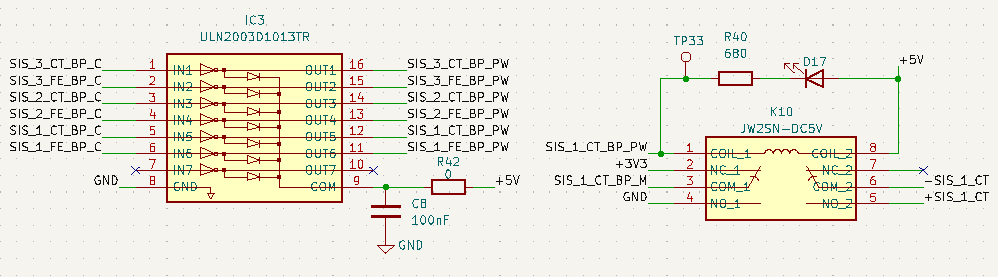
\includegraphics[width = \linewidth]{img/sis_aislamiento.png}
    \caption{Esquemático del circuito de aislamiento de un SIS}
    \label{fig:sis_aislamiento}
\end{figure}



\subsubsection{Control de señales críticas}

El SAL/T debe tener la capacidad de controlar directamente las señales críticas de control de tracción (CT) y freno de emergencia (FE). Estas señales son las más críticas que interactúan con el sistema, ya que pueden controlar el movimiento de la formación, bloquearla o permitirle el avance ignorando el estado de todos los SIS. Por estos motivos, se implementó un circuito redundado de mayor seguridad para la activación y corte de estas señales; uno para la señal de CT y otro para la señal de FE como ya se explicó que trabajan con líneas independientes. Este circuito reutiliza los conceptos del prototipo anterior explicados en su informe \cite{salt_ivan}.  \\ 

El circuito de control de las señales críticas cuenta con 2 entradas y 1 salida. Una entrada es la línea de la señal crítica después de haber pasado por las llaves interruptoras de los distintos SIS y de los circuitos de aislamiento de estos (IN); la otra entrada, es una alimentación provista por la formación capaz de energizar la electroválvula (ACT); se espera una tensión de entre 72-110V acorde a la tensión de las baterías del tren; pero al trabajar con relés, solo se va a conectar o desconectar esta señal de la línea y no se va a trabajar en su procesamiento. La salida (OUT) va directamente a la conexión con la electroválvula. En la figura \ref{fig:rele_seguridad} se observa cómo es la configuración del sistema de activación de una señal crítica respecto a los interruptores de los SIS y sus sistemas de aislamiento (expuesto de manera simplificada) y respecto a la electroválvula de la señal crítica; también se muestra el arreglo de 3 relés con sus respectivas entradas y salidas mencionadas- 

\begin{figure}[H]
    \centering
    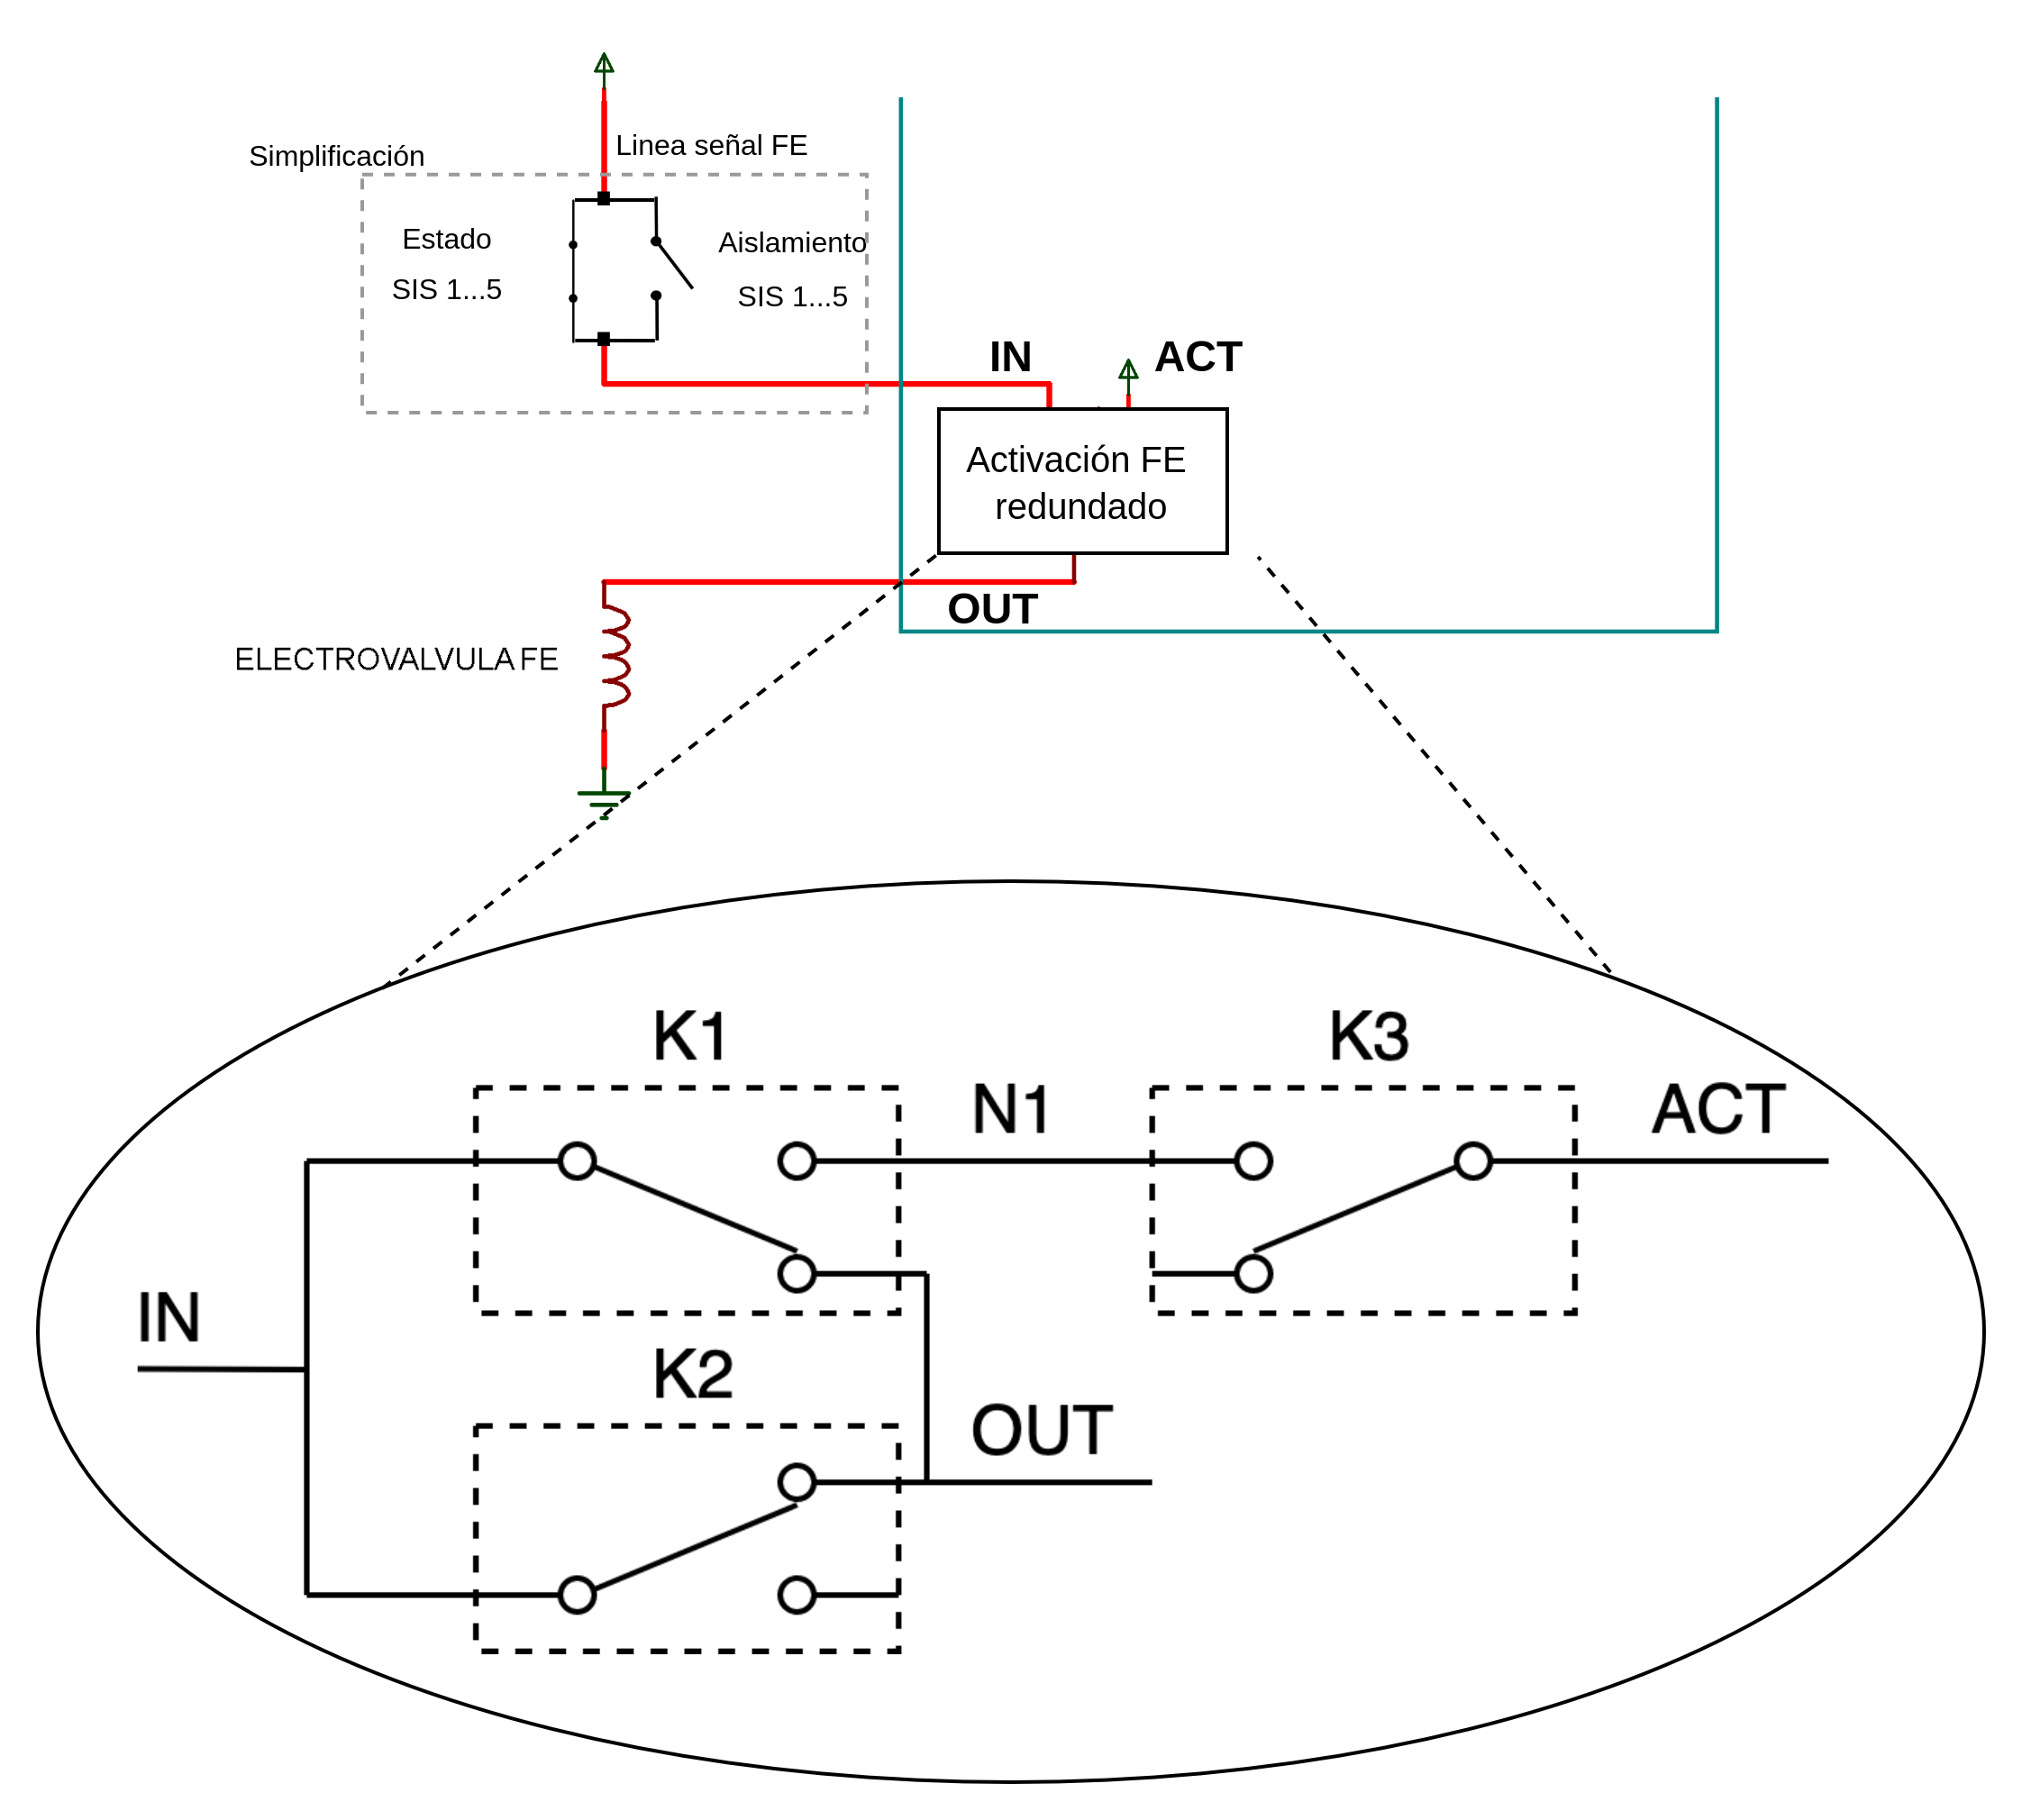
\includegraphics[width = \linewidth]{img/reles_critico.png}
    \caption{Circuito de relés redundado para activación de señales críticas}
    \label{fig:reles_critico}
\end{figure}

Para estos relés, se utilizó el mismo modelo que para el aislamiento de los SIS (JW2SN-DC5V) pero con la misma consideración que sirven de reemplazo para relés de seguridad de las mismas características de contactos. Para alimentar estos relés, se utilizó un nuevo driver de potencia ULN2003 que permite activar los 6 relés (3 para CT y 3 para FE) de estos circuitos. \\ 

Los estados del circuito se puede resumir de la siguiente manera:

\begin{itemize}
    \item \textbf{Estado normal}: El circuito no modifica la línea de la señal crítica. La entrada IN queda conectada directamente con OUT. La señal de ACT no interviene en la línea. Este estado no realiza ninguna modificación respecto a la línea tradicional sin el SAL/T y debe asegurarse que, ante una falla en el sistema, se imponga este estado dejando la activación de la señal crítica controlada por los SIS. 

    \item \textbf{Activación señal crítica o circuito abierto}: La salida OUT queda desconectada de las entradas IN y ACT. De esta manera, se asegura que el circuito queda abierto y la electroválvula quede sin alimentación lo que fuerza que la señal crítica se ejecuta. Este estado debe forzarse cuando se desea detener la formación activando el freno de emergencia o anulando el control de tracción. 

    \item \textbf{Alimentación forzada o \textit{bypass}}: La salida OUT se conecta directamente con la entrada ACT. De esta manera, la electroválvula queda alimentada independientemente de la tensión en IN y del estado de los SIS de la línea. Este estado es el más crítico porque desactiva todos los SIS de la formación y le permite el movimiento en este estado inseguro. 

\end{itemize}

Para forzar los estados mencionados, se deben controlar los relés considerando que la figura \ref{fig:reles_critico} muestra el estado normal (desenergizado) de cada uno de ellos de acuerdo a la tabla \ref{tab:estado_rele}.

\begin{table}[htb]


    \begin{tabular}{|c|c|} 
        \hline
        \textbf{Estado del circuito} & \textbf{Posición de los relés}\\
        \hline
        Estado normal     &     K1, K2 y K3 desenergizados   \\
        \hline
        Circuito abierto   &     K1 y K2 energizados. K3 desenergizado   \\
        \hline
        \textit{Bypass}   &     K1 y K3 energizados. K2 desenergizado   \\
        \hline
    \end{tabular}
\caption{Posición de relés para los estados del circuito redundado}
\label{tab:estado_rele}
\end{table}

Este sistema aumenta la seguridad de las conexiones, ya que los relés K1 y K2 cumplen una función de redundancia para volver al estado normal. En caso de que alguno de los 3 relés falle, esto significa que quede pegado en una posición no deseada, se pueden utilizar los otros 2 relés para asegurarse de volver al estado normal donde IN está conectado con OUT. Por ejemplo, si el relé K1 falla, y queda pegado conectado al nodo N1, la conexión entre IN y OUT va a seguir existiendo y no se va a generar ningún problema mientras K3 esté desenergizado. Si K2 falla, K1 conecta directamente IN y OUT. Si K3 falla, se mantiene el estado normal, ya que el nodo N1 no participa de este estado. \\ 

Al utilizar relés con dos salidas, una para este circuito de activación y otro para la medición del estado del relé, se puede detectar en todo momento cuando un relé quedó en un estado incorrecto y forzar al SAL/T en un estado de error interno restaurando la conexión normal de las señales críticas. 

\subsubsection{Registrador de eventos y conector de zona}

Las formaciones ferroviarias cuentan con un registrador de eventos que es un dispositivo que monitorea y almacena datos clave sobre el funcionamiento del tren, similar a una caja negra en aviones \cite{registrador_eventos}. Registra información como la velocidad, la activación de frenos, la posición del acelerador, el estado de las señales y otros parámetros críticos durante el viaje. Estos datos son fundamentales para analizar el rendimiento, investigar accidentes o fallos, y mejorar la seguridad operativa en el sistema ferroviario. En las formaciones para la cual se diseñó el SAL/T, se consideró la interacción con un registrador de eventos modelo Hasler Teloc 1500 \cite{hasler}. \\ 

Para el sistema SAL/T se solicitó la comunicación del estado de las siguientes características: 

\begin{itemize}    
    \item Estado de la alimentación del SAL/T
    \item Activación del modo limitado
    \item Activación del freno de emergencia
    \item Activación del corte de tracción
\end{itemize}

La comunicación con el registrador de eventos se debe realizar a través un camino de baja impedancia entre dos nodos. Para esto, se utilizó nuevamente los relés JW2SN-DC5V con un nuevo ULN2003 como driver de potencia para estos 4 relés. \\

Otra comunicación de estado que realiza el SAL/T mediante un 5to relé, también conectado al mismo driver de potencia, es con un conector de zona. Este relé debe activar un camino de baja o alta impedancia dependiendo de la zona en la que circule el tren. La ubicación es obtenida mediante GPS y, cuando se supera una distancia configurada respecto al punto de la estación de origen del recorrido, se activa un camino de baja impedancia. Esto activa en la formación un cambio en los límites de velocidad de circulación y es utilizado para formaciones que tienen parte de su recorrido en zonas rurales o menos urbanizadas. De esta manera, permite mantener distintos límites de velocidad dependiendo la zona de circulación de la formación. 
\subsubsection{Llaves de activación modo aislado limitado y total}

El SAL/T permite la activación de los modos aislado limitado (MAL) y modo aislado total (MAT) de manera local. Para el MAL, existe una llave colocada en el panel frontal del dispositivo que va a permitir la activación del modo. Para el MAT, se coloca una llave por fuera del panel frontal, instalada dentro de alguno lugar con acceso restringido al maquinista y solo accesible para el personal de mayor autoridad.  \\

La activación de estas llaves alteran completamente el funcionamiento de la formación por lo que la correcta lectura de su estado es un requisito importante para el sistema. Por esto se eligió un modelo de llave interruptora bipolar de 2 posiciones, ya que cuenta con 2 líneas y permite medir el estado en 2 entradas diferentes del MCU y asegurarse de leer la posición correcta. El modelo seleccionado es una llave interruptor Bipolar 20A de 2 posiciones de la empresa Elibet \cite{llave_elibet} que se puede visualizar en la figura \ref{fig:llave_mal} y está diseñada para ser colocada en un panel frontal. 

\begin{figure}[H]
    \centering
    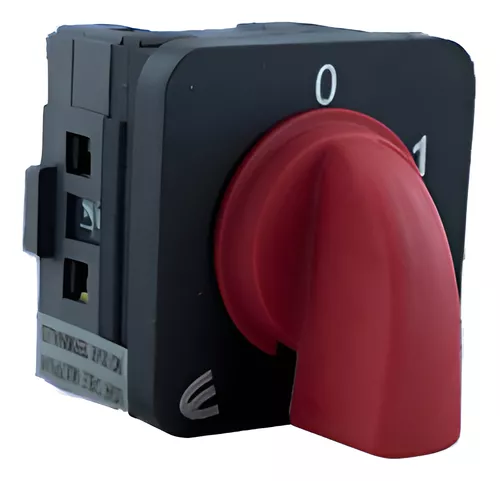
\includegraphics[width = 0.4\linewidth]{img/llave_mal.png}
    \caption{Llave interruptor bipolar 20A Elibet 0-1 posiciones}
    \label{fig:llave_mal}
\end{figure}

En la figura \ref{fig:llave_mal_sch} se muestra el circuito implementado para medir el estado de cada llave. Se conectaron resistencias de \textit{pull-up} de 40.2 K$\Omega$ y se conectaron las entradas de la llave a tierra. Cuando la llave está abierta, las señales que llegan al MCU, ON\_SW\_MAL\_1 y ON\_SW\_MAL\_2 quedan a 3V3 y el MCU toma esos nodos como entradas digitales por lo que va a detectar un estado alto. Cuando la llave se cierra, los nodos quedan conectados a tierra y el MCU va a leer un estado bajo. En caso de inconsistencia entre los valores leídos entre las 2 entradas de una misma llave, se considera el estado de no activación de la llave, ya que es el estado de mayor seguridad y no puede asegurarse el correcto funcionamiento del sistema sin una lectura correcta. 


\begin{figure}[H]
    \centering
    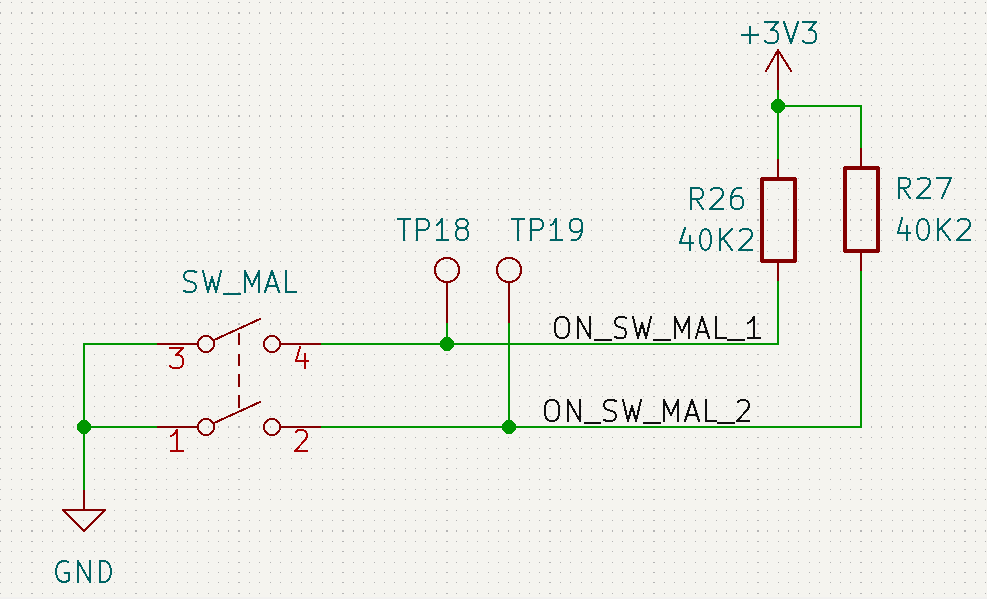
\includegraphics[width = 0.8 \linewidth]{img/llave_mal_sch.png}
    \caption{Circuito de lectura del estado de la llave interruptora}
    \label{fig:llave_mal_sch}
\end{figure}
\subsubsection{Lectura de velocidad por RS485}

El SAL/T cuenta con 3 fuentes independientes para medir la velocidad de la formación; 2 de ellas provienen de una comunicación por el protocolo RS485 con otros sistemas de la formación, la tercera proviene del módulo GPS instalado dentro del mismo SAL/T. El RS485 es un estándar de comunicación serial que permite la transmisión de datos a largas distancias y en entornos ruidosos. Utiliza un sistema de bus diferencial, lo que mejora la inmunidad al ruido y permite conectar múltiples dispositivos en una misma red.  \\ 

La fuente de medición de velocidad más confiable y por lo tanto priorizada por el SAL/T, es la indicada por el registrador de eventos Hasler Teloc 1500. La formación cuenta con un generador de pulsos ópticos Hasler que operar en el dominio infrarrojo conectado al registrador de eventos de la formación. Al mismo tiempo, el registrador de eventos está comunicado con un indicador de velocidad que tiene disponible el maquinista \cite{indicador_velocidad}. En la figura \ref{fig:hasler_teloc} se observa los dispositivos presentes en la formación. 

\begin{figure}[H]
    \centering
    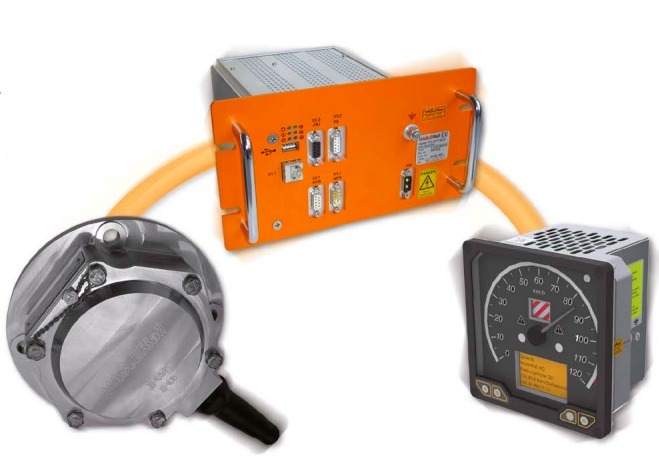
\includegraphics[width = 0.7\linewidth]{img/hasler_teloc.jpeg}
    \caption{Equipamiento Hasler en la formación ferroviaria}
    \label{fig:hasler_teloc}
\end{figure}


En el prototipo anterior del SAL/T, se realizó una tarea de ingeniería inversa para detectar cómo era la comunicación entre el registrador de eventos y el indicador de velocidad para poder interceptar esa señal y utilizar el dato de la velocidad dentro del SAL/T \cite{salt_ivan}. Revisando la documentación del equipo, con la ayuda del personal del laboratorio de material rodante de la estación de Victoria y midiendo las señales en el bus de comunicación entre estos dispositivos, se concluyó que la comunicación utilizaba el protocolo RS485 \textit{half-duplex} a 115.200 bps. Las pruebas permitieron determinar que la señal cuadrada medida utiliza una tensión de 0.5 V para el estado y de 3V3 para el estado alto. En reposo, el bus queda en estado alto y la configuración es de 8 bits con un bit extra de stop. La trama enviada está compuesta por paquetes de 31 bytes. En la figura \ref{fig:hasler_trama} se puede observar la medición de un paquete de datos completos realizado en este proceso de descubrimiento. 

\begin{figure}[H]
    \centering
    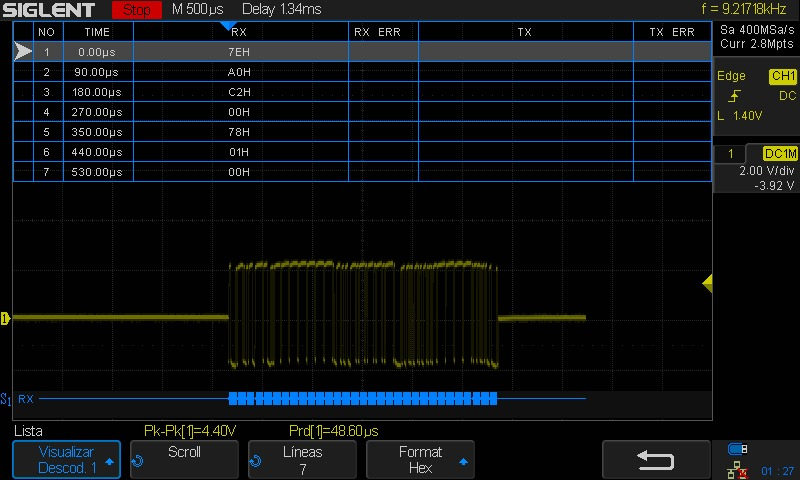
\includegraphics[width =\linewidth]{img/hasler_trama.png}
    \caption{Trama emitida por el equipo Hasler Teloc 1500}
    \label{fig:hasler_trama}
\end{figure}    

Las tramas empiezan y finalizan con un byte de start y stop de valor hexadecimal 0x7E. Conociendo el byte de start y stop es más fácil aislar las tramas y analizarlas de manera independiente. Se determinó que la información asociada a la velocidad está expresada en los bytes 7 y 8 (repetida en los bytes 9 y 10) en formato hexadecimal. También, se determinó que los bytes 29 y 30 funcionan como código de redundancia cíclica en la variante CRC-16/IBM-3740 \cite{crc}. El resto de la información contenida en la trama, no es relevante para el SAL/T como por ejemplo, la cantidad de kilómetros recorridos por la formación. \\


Por otro lado, la segunda fuente de medición de velocidad por RS485 proviene de un circuito que procesa las señales de un generador de impulsos. El generador de impulsos ópticos es un dispositivo que detecta interrupciones de un haz de luz, generalmente producido por un LED, y convierte esos cambios en señales eléctricas. Se utiliza para medir la velocidad o posición de objetos en movimiento, como ruedas o ejes, generando pulsos proporcionales a la rotación o desplazamiento. En la figura \ref{fig:pulse_generator} se puede ver el principio de funcionamiento de este dispositivo. 


\begin{figure}[H]
    \centering
    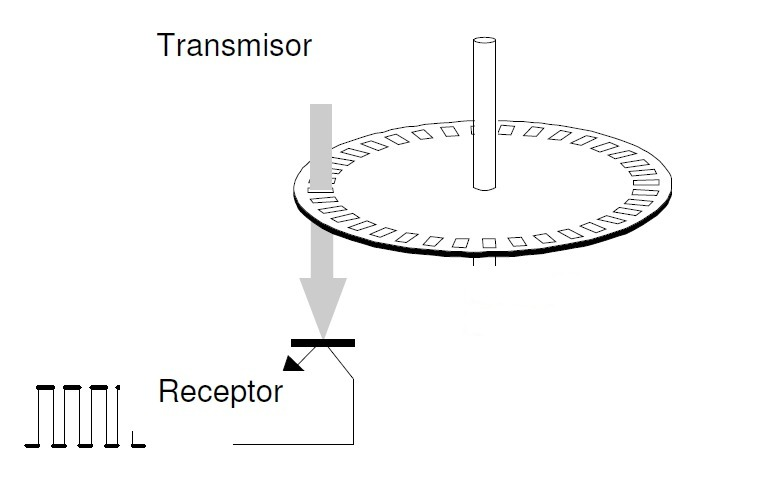
\includegraphics[width = 0.7 \linewidth]{img/pulse_generator.jpeg}
    \caption{Principio de funcionamiento de un generador de impulsos ópticos}
    \label{fig:pulse_generator}
\end{figure}    


Para determinar la velocidad a partir de la señal eléctrica, un sistema con un microcontrolador que tiene previamente configurados algunas características del generador óptico y de la formación (números de pulsos por revolución, diámetro o circunferencia de la rueda) debe considerar la frecuencia de los pulsos así como el tiempo entre pulsos para una medición más precisa de la velocidad instantánea. Una vez determinada la velocidad, este sistema externo va a montar el dato sobre un bus RS485 que se va a conectar con el SAL/T comunicando directamente el dato de la velocidad. \\ 


Dentro del SAL/T, a nivel hardware, se incluyeron dos circuitos para realizar la conversión entre el protocolo RS485 y las interfaces UART del MCU. Para armar este circuito, se tomó como referencia el circuito del mismo propósito incluido en la placa EDU-CIAA-NXP \cite{edu-ciaa}. El circuito está basado en el chip SN65HVD1176DR de Texas Instruments \cite{SN65HVD1176DR}; este es un  transceptor diferencial que trabaja en \textit{half-duplex} con características optimizadas para su uso en aplicaciones PROFIBUS \cite{profibus}. El voltaje diferencial de salida del controlador supera los requisitos de PROFIBUS de 2.1 V con una carga de 54 Ω. Una tasa de señalización de hasta 40 Mbps permite un crecimiento tecnológico hacia velocidades altas de transferencia de datos. La baja capacitancia del bus reduce la distorsión de la señal. \\

El circuito se muestra en la figura \ref{fig:rs485_sch} y se observa en la entrada las señales de recepción y trasmisión que se conectan al MCU así como un pin de salida digital que selecciona si se va a trasmitir o recibir datos ya que es un sistema \textit{half-duplex} y se comparte el bus para ambas trasmisiones. Se observan también 2 capacitores de desacople conectados en la alimentación del CI. Del lado de la salida, se colocaron las resistencias de 390 $\Omega$ y 220 $\Omega$ conocidas como \textit{bias resistors} en las recomendaciones de PROFIBUS. Por otro lado, se colocaron los \textit{jumpers} JP6, JP7 y JP8 que deben ser cortocircuitados en caso de ser el último nodo de la red. También se colocó la resistencia R22 de 100 $\Omega$ para conectar la tierra y disipar cualquier pequeña diferencia de tensión que pueda haber entre las distintas tierras de los dispositivos conectados de acuerdo a la nota de aplicación de Texas Instruments SLLA070D \cite{rs485}; esto permite reducir el ruido de modo común en las líneas de trasmisión. El circuito también utiliza el diodo supresor de transitorios (TVS) modelo SZP6SMB12CAT3G de Littelfuse \cite{SZP6SMB12CAT3G} diseñado para proteger componentes electrónicos sensibles de picos de voltaje y transitorios y el fusible reajustable MF-USMF020-2 de Bourns \cite{MF-USMF020-2} diseñado para proteger circuitos electrónicos contra sobrecorrientes. A diferencia de los fusibles tradicionales, este dispositivo puede ser reajustado manualmente después de que se ha activado, lo que proporciona una solución más conveniente y económica.




\begin{figure}[H]
    \centering
    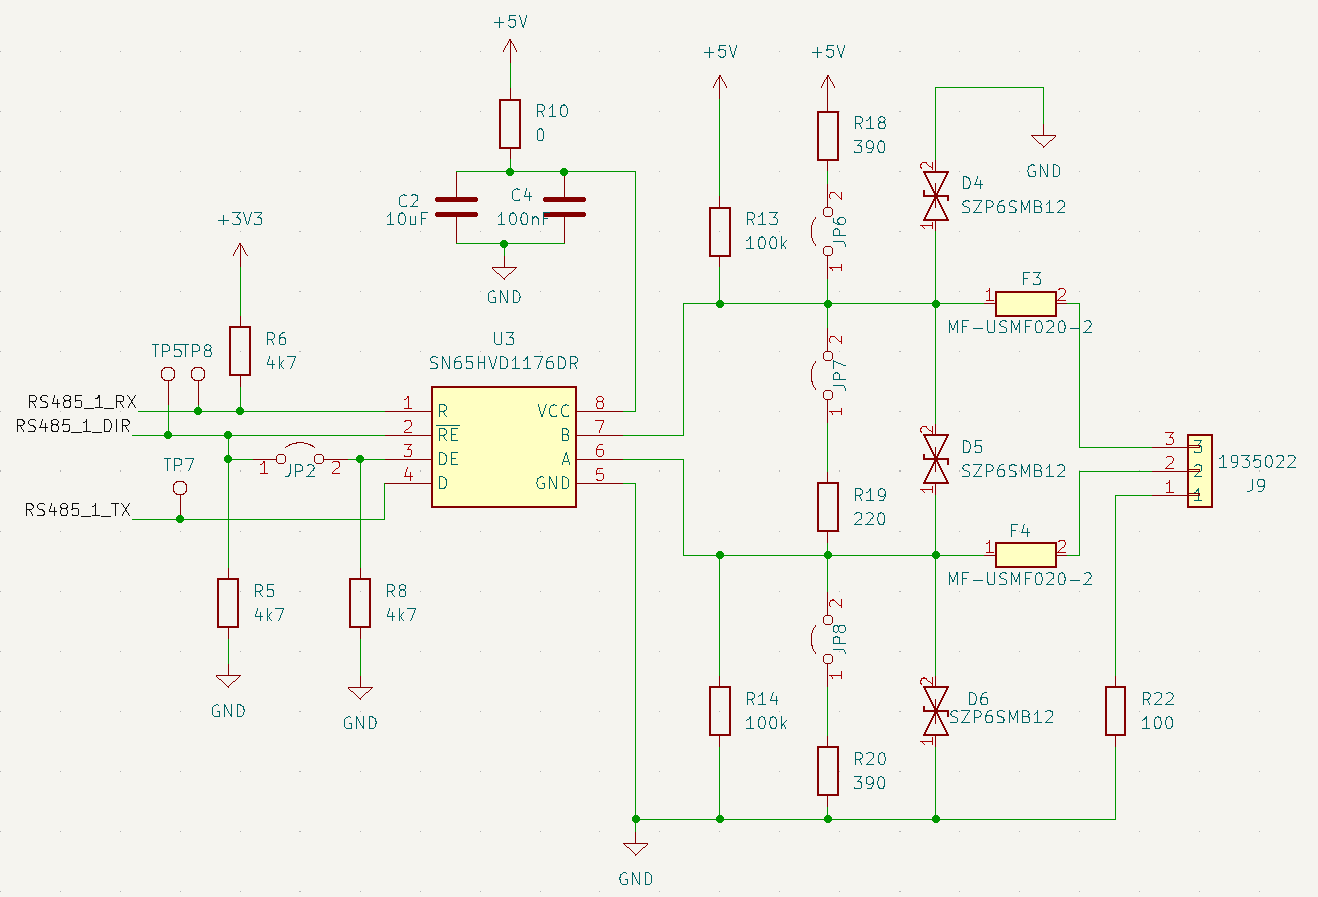
\includegraphics[width =\linewidth]{img/rs485_sch.png}
    \caption{Circuito conversor entre protocolos UART y RS485}
    \label{fig:rs485_sch}
\end{figure}    
\subsubsection{Módulo GPS}


El sistema utiliza el módulo GPS GY-NEO6MV2 para determinar la posición y velocidad del material rodante. Este módulo basado en el chip NEO-6M se alimenta con 5 V y permite la comunicación con el MCU a través de una interfaz UART. Sin embargo, no cuenta con una entrada de reset y a partir de experiencias previas de otros proyectos con módulos de estas características, se decidió armar un circuito de reset externo por en caso de detectar un error o falla en el funcionamiento del módulo. \\ 

El circuito de reset utilizado se puede observar en la figura \ref{fig:gps_sch} y utiliza el transistor MOSFET de canal P SI2343DS-T1-E3 de Vishay Semiconductors \cite{SI2343DS-T1-E3} diseñado para aplicaciones de conmutación y  control de carga en circuitos de baja potencia. Tiene una baja resistencia de encendido Rds(on) lo que permite generar una pequeña caída de tensión respecto a los 5 V que se buscan llevar al módulo. Para polarizar el circuito y permitir la circulación de corriente para encender el módulo, se debe forzar la entrada GPS\_PW\_ON a su estado bajo de 0 V. Para cortar la circulación de corriente y apagar el módulo, se debe colocar la entrada en estado de alta impedancia; esto se logra configurándolo como un pin de entrada.\\ 

\begin{figure}[H]
    \centering
    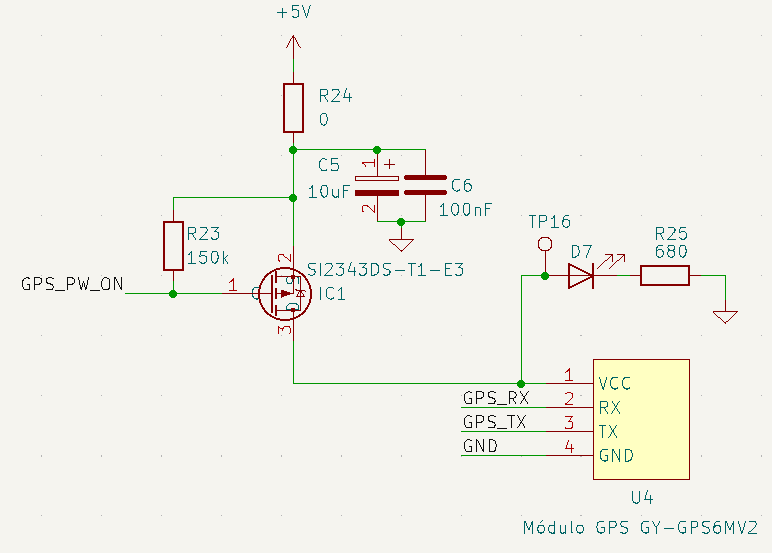
\includegraphics[width = 0.8 \linewidth]{img/gps_sch.png}
    \caption{Circuito de reset del módulo GPS}
    \label{fig:gps_sch}
\end{figure}    

Además, se agregó un LED con su respectiva resistencia para indicar cuando el módulo está alimentado y cuando no lo está, ya que el módulo no trae integrado ningún indicador luminoso. También se colocaron dos capacitores de desacople, uno electrolítico de 10 $\mu$F y otro cerámico de 100 nF para filtrar los ruidos que pueda haber en la línea de alimentación considerando también que es un módulo que trabaja con altas frecuencias y genera mayor ruido. 

\subsubsection{Módulo Wi-Fi y alimentación USB}


La comunicación del SALT con la central operativa de control se realiza utilizando la red de Internet. Para lograr esa comunicación, se utilizó el módulo ESP32 Devkit-C que tiene la capacidad de conectarse a una red Wi-Fi. Este módulo permite su alimentación con 5V ya que tiene un regulador interno que alimenta el MCU interno con 3V3. La interfaz con el SAL/T se realiza mediante el protocolo UART y se utiliza un pin GPIO para el pin de EN (\textit{enable}) que trae el módulo lo que permite forzar un reset del módulo ante cualquier falla detectada. Para facilitar la programación y el manejo de este módulo, se colocó en la placa principal un zócalo que permita insertar y remover el módulo sin necesidad de soldarlo a la placa. \\




Considerando que la formación puede no tener instalada una red Wi-Fi propia, se consideró la instalación de módulos Wi-Fi - 4G, para poder generar hasta 2 redes Wi-Fi utilizando la red de datos celular. Estos módulos utilizan las tarjetas SIM (\textit{Subscriber Identity Module}); pequeño chip utilizado en dispositivos móviles para identificar de manera única a un usuario en una red de telecomunicaciones que contiene información esencial como el número de teléfono, datos de autenticación y almacenamiento de contactos. Con estos módulos, se puede generar una red Wi-Fi utilizando la red de datos de distintos proveedores de servicio de datos celulares. Existen muchos módulos de estas características y son ampliamente utilizados en la vida cotidiana; por ejemplo, la empresa Altanet cuenta con un módem router Portátil USB 4G LTE Wi-Fi \cite{altanet} que se visualiza en la figura \ref{fig:mod_4g}. Esté módulo trabaja con todas las bandas argentinas incluyendo la banda rural y solo necesita insertarle una tarjeta nano SIM y alimentarlo por USB. 

\begin{figure}[H]
    \centering
    
\includegraphics[width = 0.3\linewidth]{img/mod_4g.png}
    \caption{Módem router Portátil USB 4G LTE Wi-Fi de Altanet}
    \label{fig:mod_4g}
\end{figure}    


En el diseño del SAL/T, se colocó en la placa dos conectores USB tipo A del modelo 87583-2010BLF de Amphenol FCI \cite{87583-2010BLF}, con los pines de alimentación conectados a 5V. Estos conectores están pensados para alimentar estos módulos Wi-Fi - 4G. Los módulos Wi-Fi -4G no fueron incluidos en el prototipo por su costo y por su fácil reemplazo por cualquier red Wi-fi generada por un router o teléfono para realizar las pruebas del sistema. 

\subsubsection{Tarjeta de almacenamiento SD}

Para incluir una tarjeta de almacenamiento SD en el sistema, se utilizó un zócalo modelo DM3AT-SF-PEJM5 de Hirose Connector \cite{DM3AT-SF-PEJM5}. Este conector admite tarjetas micro SD y tiene un sistema de \textit{push-pull} que permite manipular más fácilmente la colocación de la tarjeta. Para la tarjeta micro SD se utilizó el modelo Micro SD Ultra 8GB Clase 10 de Sandisk \cite{sd_sandisk} porque se reutilizó de otro proyecto. Sin embargo, al ser un componente de simple extracción y reemplazo, se considera que se debe utilizar una unidad de almacenaje de mayor memoria. \\

En la figura \ref{fig:sd_sch} se observa la conexión del circuito con el zócalo para micro SD. Se utilizó la interfaz SPI del MCU para la comunicación con la SD y se colocaron algunas resistencias de \textit{pull-up} recomendadas en los buses de datos o líneas desconectadas. También se incluyeron capacitores de desacople para reducir el ruido en la alimentación de la SD. El zócalo incluye además una conexión mecánica que permite determinar si existe una tarjeta colocada en el zócalo o no; esto se conecta con una entrada del MCU para poder considerar el estado físico real de la tarjeta. 



\begin{figure}[H]
    \centering
    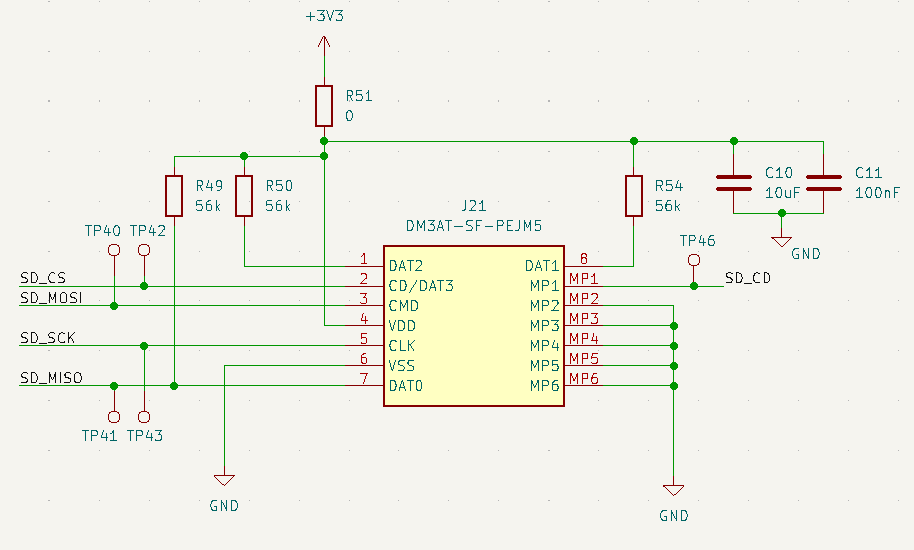
\includegraphics[width = \linewidth]{img/sd_sch.png}
    \caption{Circuito de conexión con la tarjeta SD}
    \label{fig:sd_sch}
\end{figure}    
\subsubsection{Microcontrolador y placa STM32 Nucleo-144}

El procesamiento central del sistema se realiza en el microcontrolador STM32F429ZI incluido en la placa STM32 Nucleo-144. La placa permite la alimentación del MCU y de todos sus circuitos a través de distintas entradas como se puede observar en la figura \ref{fig:nucleo_pw}. Para el SAL/T, se utilizó la entrada de E5V para alimentar la placa utilizando la fuente de alimentación del sistema y para eso se debe colocar en el JP3 un cortocircuito entre los pines 1 y 2 para tomar la tensión de allí. Se observa que la placa incluye un circuito de regulación de tensión a 3V3 para alimentar el MCU y otros circuitos internos. 


\begin{figure}[H]
    \centering
    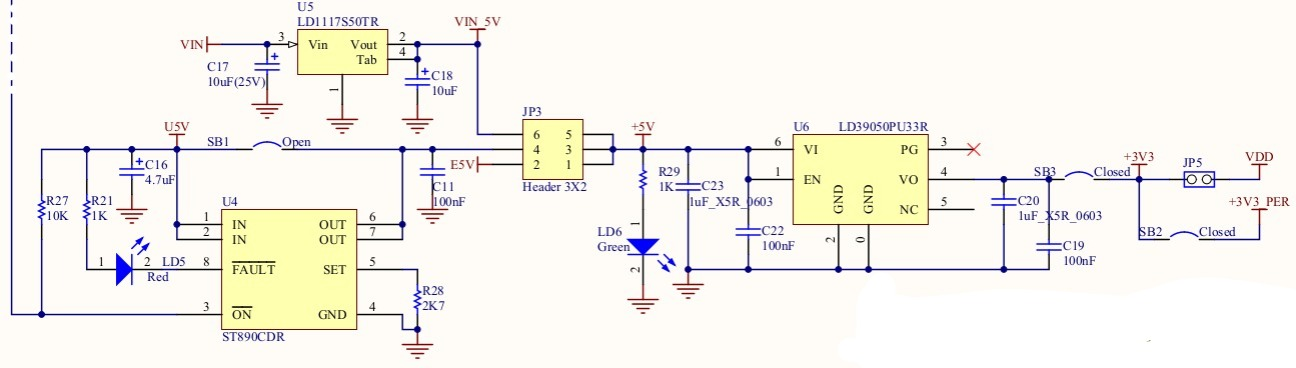
\includegraphics[width = \linewidth]{img/nucleo_pw.jpeg}
    \caption{Esquemático de la alimentación de la placa STM32 Nucleo-144}
    \label{fig:nucleo_pw}
\end{figure}    

Para la inserción de la STM32 Nucleo-144 en la placa principal del SAL/T, se utilizaron los conectores de expansión morpho que permiten el acceso a todos los pines del MCU al usuario. Para eso, se soldaron los pines en la Nucleo y se colocaron conectores hembra en la placa principal. Se necesitaron 2 conectores de 2x36 pines cada uno para conectar la placa. Este tipo de conectores permite colocar y sacar la placa fácilmente lo que permite manipularla mejor para la programación y cualquier prueba de circuitos que se quiera realizar sin la placa colocada. En la figura \ref{fig:diagrama_bloques_coms} se mostraron las distintas interfaces utilizadas del microcontrolador en las que se incluye ADC, SPI, UART, I2C y GPIO. 
\subsubsection{Panel frontal}


El panel frontal del SAL/T sigue el diseño de la figura \ref{fig:panel_frontal} utilizando una placa secundaria donde se colocan directamente los LEDs (\textit{Light-Emitting Diode}), el display de velocidad, el botón seleccionador de perfil intermitente y un buzzer sonoro. \\ 

El panel frontal cuenta con cuatro LEDs verdes utilizados para indicar el estado de la alimentación, el modo aislado limitado, el modo aislado total y el perfil intermitente seleccionados; diez LEDs RGB (\textit{Red Green Blue}) para indicar el estado de los SIS, de las señales de CT y FE, la presencia de un comando remoto activo, el estado del receptor GPS y un indicador de la zona de circulación actual de la formación; un botón para seleccionar el perfil intermitente a utilizar; el display de velocidad de cuatro dígitos 7 segmentos y la llave interruptora que queda por fuera de la placa secundaria. \\ 

Para controlar todos estos LEDs y el display de velocidad, se utilizó el controlador LED AS1115-BSST de ams OSRAM \cite{AS1115-BSST}. Este permite controlar hasta sesenta y cuatro LEDs u ocho dígitos de un display 7 segmentos reduciendo la cantidad de pines necesarios a utilizar del MCU ya que se conecta por protocolo I2C utilizando solamente dos cables. Este controlador permite setear la corriente de cada LED utilizando una resistencia externa; en este caso, siguiendo los valores normalizados y recomendados por la hoja de datos del controlador, se colocó una resistencia de 22 k$\Omega$ para obtener una corriente de 10 mA. El controlador también trae entradas para la detección de hasta dieciséis teclas en una matriz de teclas, pero esa funcionalidad no se utiliza en esta aplicación. \\



El AS1115-BSST utiliza un método de multiplexado en el cual cada grupo de LEDs o segmentos es controlado secuencialmente, encendiéndolos en rápida sucesión. Esto reduce la cantidad de pines necesarios para el control, ya que todos los LEDs no están encendidos simultáneamente, pero debido a la alta velocidad de escaneo, se perciben como si estuvieran encendidos de forma continua. Además, a través de la interfaz I2C, se envían comandos para controlar el brillo, encendido y apagado de los LEDs o segmentos, y se pueden ajustar los valores de corriente para mejorar la eficiencia energética.\\




En la figura \ref{fig:led_driver} se observa una aplicación típica de este controlador; para el SAL/T, se utilizó una alimentación de 5 V, un Rset = 22 k$\Omega$, la comunicación con el MCU solo con las líneas de SDA y SCL de I2C trabajando a 100 kHz sin el pin de interrupción, no se utilizaron las entradas de detección de teclas, y se conectó al display de cuatro dígitos 7 segmentos y a los LEDs mencionados previamente. \\

\begin{figure}[H]
    \centering
    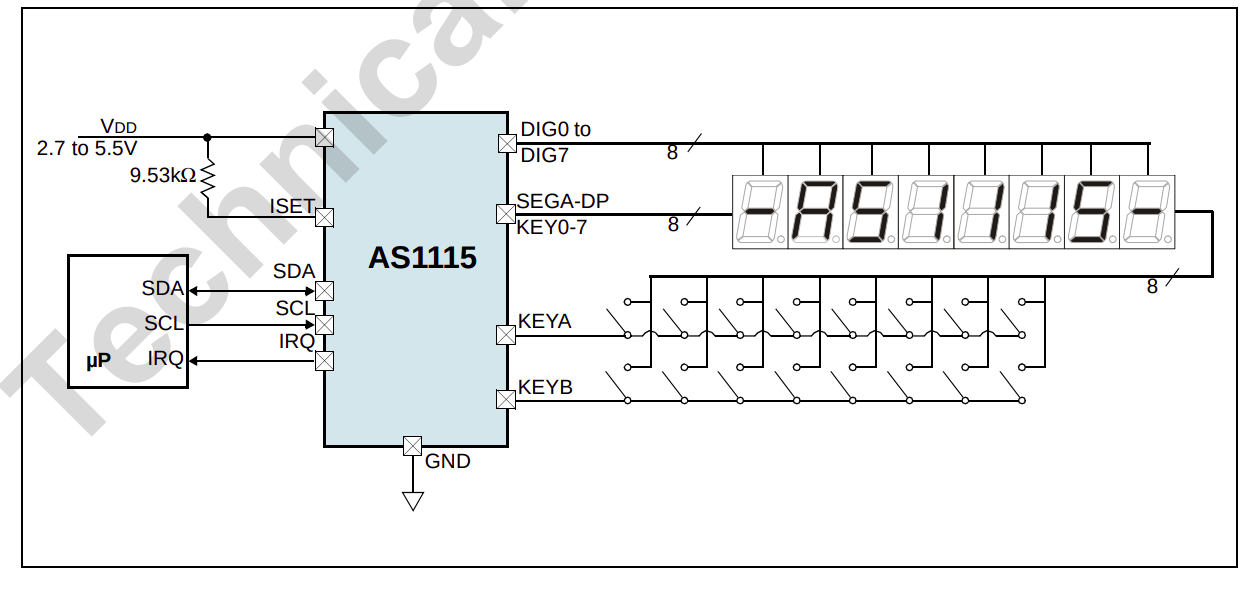
\includegraphics[width = \linewidth]{img/led_driver.png}
    \caption{Aplicación típica de un controlador AS1115-BSST}
    \label{fig:led_driver}
\end{figure}    




Para los LEDs RGB utilizados se seleccionó el modelo WP154A4SEJ3VBDZGW/CA de Kingbright \cite{WP154A4SEJ3VBDZGW/CA} diseñado para aplicaciones que requieren indicación de estado multicolor. Ofrece alta luminosidad y bajo consumo de energía, con un encapsulado transparente de 5 mm, lo que lo hace ideal para proyectos que requieren señalización visual con múltiples colores en un solo componente. Trabajan con una corriente máxima de 20 mA por color, y tienen una caída de tensión e intensidad luminosa para cada color de: 

\begin{itemize}
    \item Rojo: 2 V - 300 mcd
    \item Verde: 3,3 V - 600 mcd
    \item Azul: 3,3 V - 500 mcd
\end{itemize}

Estos LEDs se montan \textit{through hole} y quedan sobresalientes a la placa para luego insertarlos dentro de un gabinete con agujeros para permitir la visualización de estos componentes. Tienen un encapsulado transparente y un lente de tipo redondo con un ángulo de visión de 30°.\\ 

Para los LEDs verdes se utilizó el modelo WP7113LZGCK de Kingbright \cite{WP7113LZGCK} que cuenta con características muy similares solo para el color verde del modelo RGB presentado. Las diferencias son que tiene una tensión Vf = 2,1 V, tolera una corriente máxima de 30 mA y su intensidad luminosa es un poco mayor, ya que puede llegar hasta 3000 mcd dependiendo de la corriente. \\ 

Para el display de velocidad se utilizó el modelo LTC-5723HR de Lite-On \cite{LTC-5723HR}; contiene cuatro dígitos con formato de 7 segmentos de color rojo en configuración cátodo común. Cada dígito tiene un tamaño de 8,1 x 14,2 mm. Funciona con una tensión directa de Vf = 2 V y corriente de hasta 20 mA por segmento. Es de montaje \textit{through-hole} lo que permite dejarlo visible por fuera de la placa con cierta separación. \\

En la figura \ref{fig:leds_model} se visualiza el display mencionado junto a un LED RGB y un LED verde utilizado para la implementación. 

\begin{figure}[H]
    \centering
    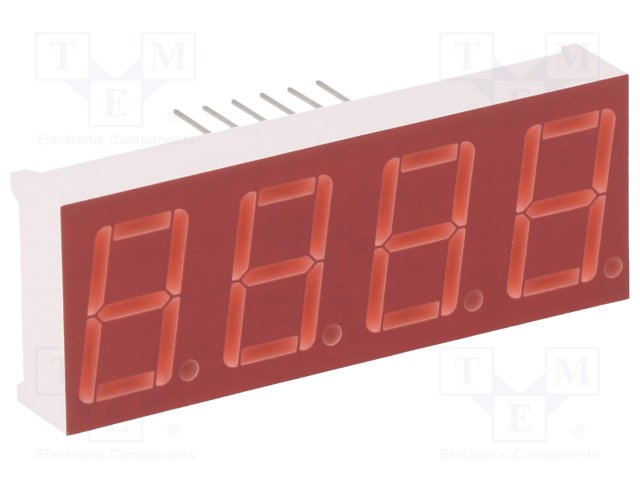
\includegraphics[width = 0.3 \linewidth]{img/display.jpg}
    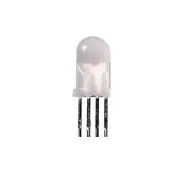
\includegraphics[width = 0.3 \linewidth]{img/led_rgb.png}
    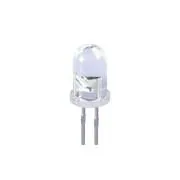
\includegraphics[width = 0.3 \linewidth]{img/led_g.png}
    \caption{Modelos utilizados para las indicaciones luminosas del panel frontal}
    \label{fig:leds_model}
\end{figure}    


Para el botón de selección del perfil intermitente se utilizó un interruptor con pulsador \textit{push switch} modelo de 1543-650-149 de Bourns \cite{1543-650-149} utilizando un circuito con una resistencia de \textit{pull-down} para forzar 0 V en la entrada del MCU cuando el interruptor está abierto y una resistencia para realizar un divisor resistivo de 5 V (alimentación de la placa) a 3,3 V (tensión de nivel alto de entrada digital del MCU). También se agregó una resistencia en serie de 100 Ohms. En la figura \ref{fig:chop_sel} se visualiza el circuito. 

\begin{figure}[H]
    \centering
    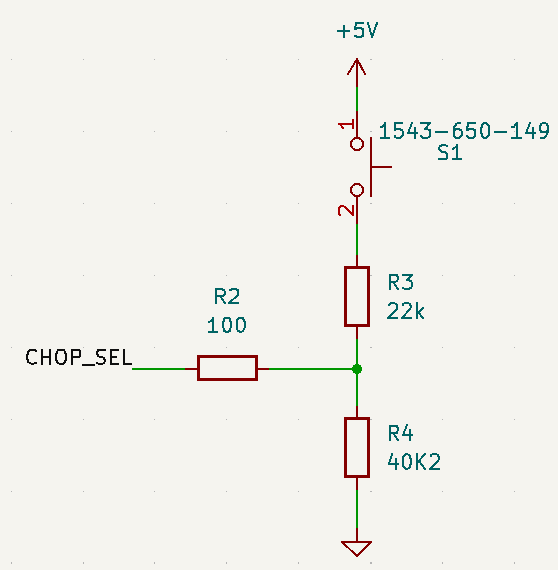
\includegraphics[width = 0.5 \linewidth]{img/chop_sel.png}
    \caption{Circuito del selector de perfil intermitente}
    \label{fig:chop_sel}
\end{figure}    


El panel frontal cuenta también con un buzzer sonoro que se activa de manera intermitente cuando se circula en modo aislado limitado y suena de manera continua cuando se exceden los límites de velocidad establecidos. Para el buzzer sonoro se utilizó el modelo CEM-1205-IC de SameSky \cite{CEM-1205-IC}. Este módulo cuenta con un oscilador interno que al energizarse con 5 VDC emite una señal sonora de 2400 Hz consumiendo 30 mA de corriente. Para el control del encendido de este módulo, se utilizó un transistor MOSFET canal P modelo NVTR0202PLT1G de onsemi \cite{NVTR0202PLT1G} conectado como se visualiza en la figura \ref{fig:buzzer_sch}. Cuando la señal de control BUZZER\_C está en estado bajo 0 V, el circuito permite la corriente y alimenta el buzzer sonoro; cuando la señal se coloca en un estado de alta impedancia, no circula corriente apagando el buzzer sonoro. También se colocó un capacitor de 10 $\mu$F para suavizar el sonido reduciendo los ruidos que puedan entrar por la línea de alimentación. 



\begin{figure}[H]
    \centering
    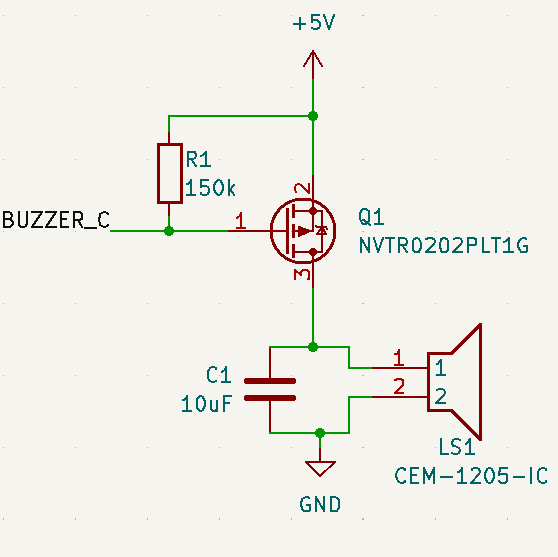
\includegraphics[width = 0.6 \linewidth]{img/buzzer.png}
    \caption{Circuito de activación del buzzer sonoro}
    \label{fig:buzzer_sch}
\end{figure}    



\subsubsection{Fabricación y ensamblado}

El diseño de hardware del SAL/T incluye algunos otros componentes no mencionados en los puntos anteriores. Las resistencias utilizadas en el proyecto son resistencias de película gruesa de montaje superficial (SMD), de 1/4 W, tolerancia del 1\% y tamaño 0805; se utilizaron los distintos valores que ofrece la empresa YAGEO para su serie RC. Para los capacitores se utilizaron generalmente capacitores cerámicos multicapa de KEMET, de montaje superficial tamaño 0805, tolerancia del 10\% y operan hasta 16 VDC. Para los capacitores electrolíticos, se utilizaron capacitores de aluminio de Panasonic de la serie HA con tolerancia 20\% y operación hasta 35 VDC. \\ 

En la tabla \ref{tab:bom}, se visualiza el listado completo de los componentes (BOM) necesarios para fabricar el prototipo del SAL/T con sus precios en dólares estadounidenses expuestos por el distribuidor Mouser Electronics que suma un total de 362.97 USD: 

\begin{table}[H]
\begin{tabular}{|c|c|c|c|c|c|}
 \hline
 & Fabricante          & Modelo                                                                                                                                                                                                                                    & Cantidad & Precio & Precio \\ 
 
 &           &                                                                                                                                                                                                                                     &  & unitario & del item \\ 
 \hline
1                    & KEMET               & \href{https://ar.mouser.com/datasheet/2/447/KEM_C1002_X7R_SMD-3316098.pdf}{C1206C106K4RACTU}                                                                                                                        & 5        & 0,35            & 1,75            \\ \hline
2                    & KEMET               & \href{https://ar.mouser.com/datasheet/2/447/KEM_C1002_X7R_SMD-3316098.pdf}{C0805C104K4RACTU}                                                                                                                        & 25       & 0,14            & 3,50            \\ \hline
3                    & Panasonic           & \href{http://industrial.panasonic.com/cdbs/www-data/pdf/RDE0000/ABA0000C1148.pdf}{EEE-HAV100WAR}                                                                                                                       & 3        & 0,38            & 1,13            \\ \hline
4                    & LITTELFUSE          & \href{https://www.littelfuse.com/$\sim$/media/electronics/datasheets/tvs_diodes/littelfuse_tvs_diode_szp6smb_datasheet.pdf.pdf}{SZP6SMB12CAT3G}                                                                   & 6        & 0,43            & 2,58            \\ \hline
5                    & Wurth Elektronik    & \href{https://www.we-online.com/catalog/datasheet/150080VS75000.pdf}{150080VS75000}                                                                                                                                    & 22       & 0,19            & 4,11            \\ \hline
6                    & Lite-On             & \href{https://componentsearchengine.com/Datasheets/1/LTC-5723HR.pdf}{LTC-5723HR}                                                                                                                                       & 1        & 2,99            & 2,99            \\ \hline
7                    & Bourns              & \href{https://www.bourns.com/docs/Product-Datasheets/mfusmf.pdf}{MF-USMF020-2}                                                                                                                                         & 4        & 0,34            & 1,36            \\ \hline
8                    & Vishay              & \href{https://www.vishay.com/docs/72079/si2343ds.pdf}{SI2343DS-T1-E3}                                                                                                                                                  & 1        & 0,75            & 0,75            \\ \hline
9                    & STMicroelectronics  & \href{http://www.st.com/st-web-ui/static/active/en/resource/technical/document/datasheet/CD00001244.pdf}{ULN2003D1013TR}                                                                                               & 4        & 0,73            & 2,91            \\ \hline
10                   & Texas Instruments   & \href{https://www.ti.com/lit/ds/symlink/ina823.pdf}{INA823DGKR}                                                                                                                                                        & 10       & 2,35            & 23,50           \\ \hline
11                   & Renesas Electronics & \href{https://www.renesas.com/en-us/www/doc/datasheet/icl7660s-a.pdf}{ICL7660AIBAZA}                                                                                                                                   & 1        & 2,03            & 2,03            \\ \hline
12                   & ams                 & \href{https://datasheet.datasheetarchive.com/originals/distributors/Datasheets-SFU1/DSASFU10002655.pdf}{AS1115-BSST}                                                                                                   & 1        & 6,58            & 6,58            \\ \hline
13                   & Phoenix Contact     & \href{http://www.phoenixcontact.com/de/produkte/1757491/pdf}{1757491}                                                                                                                                                  & 8        & 1,32            & 10,56           \\ \hline
14                   & Phoenix Contact     & \href{http://www.phoenixcontact.com/de/produkte/1757488/pdf}{1757488}                                                                                                                                                  & 11       & 1,06            & 11,66           \\ \hline
15                   & Amphenol FCI        & \href{https://ar.mouser.com/datasheet/2/18/1/87583-2579162.pdf}{87583-2010BLF}                                                                                                                                         & 2        & 1,07            & 2,14            \\ \hline
16                   & Hirose              & \href{https://datasheet.lcsc.com/szlcsc/Hirose-HRS-DM3AT-SF-PEJM5_C114218.pdf}{DM3AT-SF-PEJM5}                                                                                                                        & 1        & 2,63            & 2,63            \\ \hline
17                   & Phoenix Contact     & \href{http://www.phoenixcontact.com/de/produkte/1757475/pdf}{1757475}                                                                                                                                                  & 1        & 0,73            & 0,73            \\ \hline
18                   & SparkFun            & \href{https://cdn.sparkfun.com/assets/1/c/f/7/9/DS-16581-Female_Header_2x18.pdf}{PRT-09044}                                                                                                                          & 8        & 0,38            & 3,04            \\ \hline
19                   & Panasonic           & \href{https://www3.panasonic.biz/ac/e_download/control/relay/power/catalog/mech_eng_jw.pdf}{JW2SN-DC5V}                                                                                                             & 21       & 2,10            & 44,10           \\ \hline
20                   & Kingbright          & \href{https://www.mouser.com/datasheet/2/216/WP7113LZGCK-535810.pdf}{WP7113LZGCK}                                                                                                                                      & 8        & 0,36            & 2,89            \\ \hline
21                   & Kingbright          & \href{http://www.kingbrightusa.com/images/catalog/SPEC/WP154A4SEJ3VBDZGW-CA.pdf}{WP154A4SEJ3VBDZGW/CA}                                                                                                                 & 10       & 1,36            & 13,60           \\ \hline
22                   & CUI Devices         & \href{https://www.cuidevices.com/product/resource/cem-1205-ic.pdf}{CEM-1205-IC}                                                                                                                                        & 1        & 1,91            & 1,91            \\ \hline
23                   & onsemi              & \href{https://componentsearchengine.com/Datasheets/2/NVTR0202PLT1G.pdf}{NVTR0202PLT1G}                                                                                                                                 & 1        & 0,38            & 0,38            \\ \hline
24                   & YAGEO               & \href{https://ar.mouser.com/datasheet/2/447/PYu_RC_Group_51_RoHS_L_11-1984063.pdf}{RC0805FR-104K7L}                                                                                                              & 6        & 0,10            & 0,60            \\ \hline
25                   & YAGEO               & \href{https://ar.mouser.com/datasheet/2/447/YAGEO_PYu_RC_Group_51_RoHS_L_12-3313492.pdf}{RC0805FR-10100KL}                                                                                                      & 4        & 0,10            & 0,40            \\ \hline
26                   & YAGEO               & \href{https://ar.mouser.com/datasheet/2/447/YAGEO_PYu_RC_Group_51_RoHS_L_12-3313492.pdf}{RC0805FR-07390RL}                                                                                                      & 4        & 0,10            & 0,40            \\ \hline
27                   & YAGEO               & \href{https://ar.mouser.com/datasheet/2/447/PYu_RC_Group_51_RoHS_L_11-1984063.pdf}{RC0805FR-13220RL}                                                                                                             & 2        & 0,10            & 0,20            \\ \hline
28                   & YAGEO               & \href{https://ar.mouser.com/datasheet/2/447/PYu_RC_Group_51_RoHS_L_11-1984063.pdf}{RC0805FR-10100RL}                                                                                                             & 3        & 0,02            & 0,05            \\ \hline
29                   & YAGEO               & \href{https://ar.mouser.com/datasheet/2/447/PYu_RC_Group_51_RoHS_L_11-1984063.pdf}{RC0805FR-13150KL}                                                                                                             & 2        & 0,10            & 0,20            \\ \hline
30                   & YAGEO               & \href{https://ar.mouser.com/datasheet/2/447/PYu_RC_Group_51_RoHS_L_11-1984063.pdf}{RC0805FR-13680RL}                                                                                                             & 22       & 0,10            & 2,20            \\ \hline
31                   & YAGEO               & \href{https://ar.mouser.com/datasheet/2/447/YAGEO_PYu_RC_Group_51_RoHS_L_12-3313492.pdf}{RC0805FR-0740K2L}                                                                                                      & 5        & 0,10            & 0,50            \\ \hline
32                   & YAGEO               & \href{https://ar.mouser.com/datasheet/2/447/PYu_RC_Group_51_RoHS_L_11-1984063.pdf}{RC0805FR-1056KL}                                                                                                              & 3        & 0,10            & 0,30            \\ \hline
33                   & YAGEO               & \href{https://ar.mouser.com/datasheet/2/447/PYu_RC_Group_51_RoHS_L_11-1984063.pdf}{RC0805FR-101ML}                                                                                                               & 20       & 0,10            & 2,00            \\ \hline
34                   & YAGEO               & \href{https://ar.mouser.com/datasheet/2/447/YAGEO_PYu_RC_Group_51_RoHS_L_12-3313492.pdf}{RC0805FR-0730KL}                                                                                                       & 20       & 0,10            & 2,00            \\ \hline
35                   & YAGEO               & \href{https://ar.mouser.com/datasheet/2/447/PYu_RC_Group_51_RoHS_L_11-1984063.pdf}{RC0805FR-1022KL}                                                                                                              & 2        & 0,10            & 0,20            \\ \hline
36                   & Bourns              & \href{https://www.arrow.com/en/products/1543-650-149/bourns}{1543-650-149}                                                                                                                                             & 1        & 1,21            & 1,21            \\ \hline
37                   & STMicroelectronics  & \href{https://ar.mouser.com/datasheet/2/389/nucleo_l496zg-1848160.pdf}{NUCLEO-F429ZI}                                                                                                                                 & 1        & 24,47           & 24,47           \\ \hline
38                   & Texas Instruments   & \href{http://www.ti.com/lit/gpn/sn65hvd1176}{SN65HVD1176DR}                                                                                                                                                            & 2        & 2,94            & 5,88            \\ \hline
39                   & u-Blox              & \href{https://www.datasheethub.com/gy-neo6mv2-flight-control-gps-module/}{GPS GY-NEO6MV2}                                                                                                                              & 1        & 13,48           & 13,48           \\ \hline
40                   & Espressif Systems   & \href{https://docs.espressif.com/projects/esp-idf/en/latest/esp32/hw-reference/esp32/get-started-devkitc.html}{ESP32-DevKitC-32E}                                                                                      & 1        & 13,87           & 13,87           \\ \hline
41                   & Harwin              & \href{https://ar.mouser.com/datasheet/2/181/M20-977-1220590.pdf}{M20-9774046}                                                                                                                                          & 6        & 1,47            & 8,82            \\ \hline
42                   & Elibet              & \href{https://articulo.mercadolibre.com.ar/MLA-715063582-llave-interruptor-bipolar-20a-elibet-0-1-panel-_JM\#position=4\&search_layout=stack\&type=item\&tracking_id=a983e77f-e6e3-4bab-bc34-8ba853ec8955}{20002/0} & 2        & 10,60           & 21,20           \\ \hline
43                   & Altanet             & \href{https://www.voipexperts.com.ar/index.php?option=com_k2\&Itemid=136\&id=953_bc11baf33c1825b2df10adc8c4f9a628\&lang=es\&task=download\&view=item}{AltaNet Stick ST10 4G WiFi}                                    & 2        & 44,77           & 89,54           \\ \hline
44                   & Phoenix Contact     & \href{https://www.phoenixcontact.com/us/products/1934887/pdf}{1934887}                                                                                                                                                 & 8        & 1,00            & 7,96            \\ \hline
45                   & Phoenix Contact     & \href{https://www.phoenixcontact.com/us/products/1935022/pdf}{1935022}                                                                                                                                                 & 11       & 0,71            & 7,77            \\ \hline
46                   & Phoenix Contact     & \href{https://www.phoenixcontact.com/us/products/1934861/pdf}{1934861}                                                                                                                                                 & 1        & 0,55            & 0,55            \\ \hline
47                   & Samtex              & \href{https://www.mouser.fr/datasheet/2/527/ssw_th-2854740.pdf}{SSW-119-01-T-S}                                                                                                                                       & 2        & 2,44            & 4,88            \\ \hline
48                   & Adam Tech           & \href{https://www.mouser.fr/datasheet/2/4/rs1_xx_g_data_sheet-3396051.pdf}{RS1-04-G}                                                                                                                               & 1        & 0,23            & 0,23            \\ \hline
49                   & SparkFun            & \href{https://www.mouser.fr/ProductDetail/SparkFun/PRT-16581?qs=sPbYRqrBIVmf2mq2gyI4eA\%3D\%3D}{PRT-16581}                                                                                                             & 4        & 1,81            & 7,24       \\ \hline

\end{tabular}
\caption{Listado de componentes del SAL/T}
\label{tab:bom}
\end{table}



Con el listado de materiales y sus hojas de datos presentes (que pueden ser accedidas mediante el hipervínculo colocado sobre cada modelo de componente en la tabla \ref{tab:bom}), se calculó el consumo máximo de potencia del SAL/T. La potencia total máxima que puede consumir el sistema, considerando que todos los componentes están trabajando al máximo de consumo lo que es un caso improbable, es de 18.38 W. El principal componente de la potencia son los relés que individualmente consumen 106mA cada uno al estar activados y hay 21 relés en todo el sistema. Los módulos USB Wi-Fi-4G, considerados para el cálculo de potencia, también tienen un gran consumo de 500mA cada uno, ya que necesitar generar la señal de la red Wi-Fi. Los módulos de GPS, ESP32 y Nucleo consumen alrededor de 100mA cada uno. El resto de los componentes suman de manera insignificante al número total. Por eso, se considera necesario una fuente de 5V con potencia de 20W para alimentar el SAL/T. \\


El diseño del sistema considera para todos los circuitos integrados un capacitor de 100nF de desacople para conectar cerca de su pin de alimentación entre VCC y tierra con el objetivo de filtrar ruidos que puedan estar presentes en la línea de alimentación. Para los casos más sensibles, también se contempló un capacitor electrolítico de 10 $\mu$F con la idea de reforzar el filtrado para ruidos de distintas frecuencias. También, en los esquemáticos se colocó una resistencia de 0 $\Omega$ al previo a conectar la línea de alimentación con el pin VCC de los chips para permitir el armado progresivo y segmentado del circuito una vez fabricado.  La selección de componentes consideró utilizar la menor cantidad posible de componentes \textit{through-hole} priorizando los de montaje superficial porque en aplicaciones ferroviarias, los componentes \textit{through-hole} pueden sufrir cortes o daños por las vibraciones de la formación.\\

Para conectar los módulos a la placa, se eligió utilizar conectores hembra tipo zócalo soldados a la placa para permitir colocar y sacar los módulos de manera más simple para su manipulación, programación y eventual reemplazo. Para la conexión con los sistemas externos, se utilizaron conectores de tipo bornera con tornillo soldados a la placa que permiten la conexión de cables. El sistema cuenta con 20 borneras en total y es por eso que cada una tiene identificada su función así como cada pin tiene indicada a qué señal corresponde. Esto aplica también para todos los componentes del sistema que tienen señalado qué número de componente corresponde a cada \textit{footprint} para facilitar el armado y el mantenimiento de las placas ante cualquier inconveniente. También se colocaron puntos de prueba en la mayoría de las señales relevantes para el sistema para poder medir el estado eléctrico de cada señal durante el armado, \textit{debugging} y pruebas del sistema. \\



Se intentó utilizar anchos de pista grandes para evitar quiebres en las pistas por vibraciones o flexiones de la placa y reducir la resistencia de las pistas también fue necesario utilizar distintos anchos para poder realizar el ruteo entre pines de la placa Núcleo. Se utilizaron anchos de .3mm, .4mm, .5mm y .8mm considerando el mayor ancho para las señales de alimentación o que transportan mayor corriente. Las vías se hicieron de 1mm con agujero de .4mm. Para los conectores de las borneras, se siguió la recomendación de utilizar agujeros grandes de 3mm/1.4mm y pistas anchas de .8mm para reducir el daño que pueda causar las fricciones provocadas por el procedimiento de instalación utilizando los tornillos de la bornera. Los puntos de prueba se hicieron de 1.53mm/1.02 para permitir utilizar la punta de un tester común para medir las señales. Además, las placas cuentan con agujeros para el montaje de la placa en el gabinete que se hicieron siguiendo el formato de tornillo M3 de diámetro 3.2mm. \\

En la tabla \ref{tab:design_constraints} se visualizan algunas de las restricciones utilizadas como reglas de diseño:

\begin{table}[H]
    \centering
    \begin{tabular}{|c|c|}
        \hline
         \textbf{Restricción} & \textbf{Valor}  \\ \hline
         Cobre - mínima distancia entre pistas & 0.2mm  \\ \hline
         Cobre - mínimo ancho de pista & 0.3mm  \\ \hline
         Cobre - mínimo ancho anular  & 0.25mm  \\ \hline
         Cobre - mínimo diámetro de vía  & 1mm  \\ \hline
         \textit{Holes} - mínimo diámetro del agujero & 0.3mm \\ \hline
         \textit{Holes} - mínimo distancia entre agujeros & 0.254mm \\
         \hline
    \end{tabular}
    \caption{Restricciones de diseño utilizadas para el diseño del PCB}
    \label{tab:design_constraints}
\end{table}


En ambas placas, se utilizó una de las capas como plano de tierra intentando utilizar la menor cantidad de pistas por ese lado mientras que la otra capa se utilizó para hacer todas las conexiones posibles. En las figuras \ref{fig:salt_tracks} y \ref{fig:salt_ihm_tracks} se visualiza los trazos de las pistas diseñados en ambas placas: 


\begin{figure}[H]
    \centering
    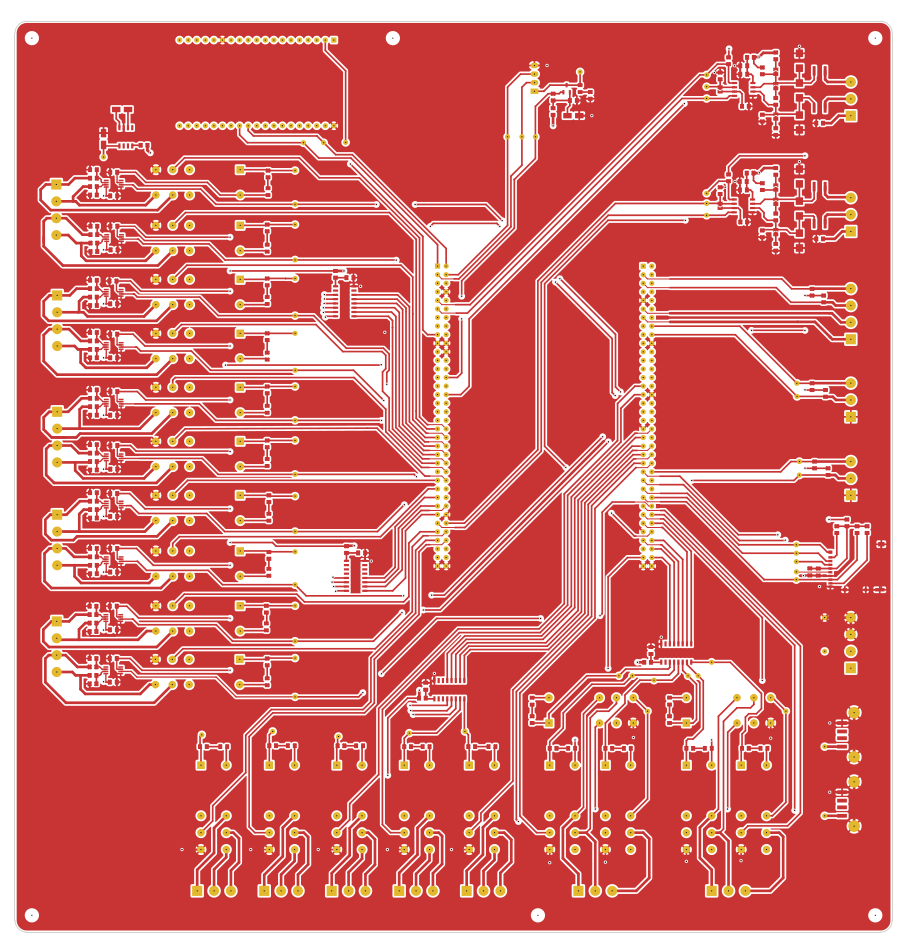
\includegraphics[width = 0.49\linewidth]{img/salt_tracks_front.png}
    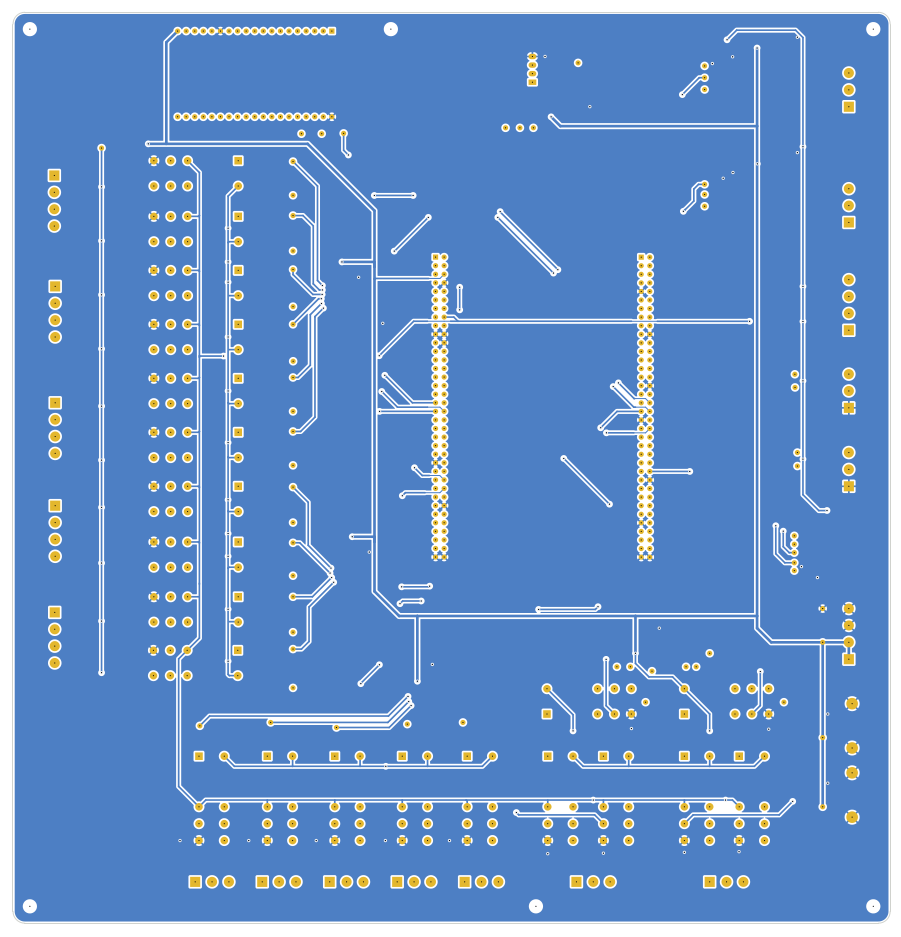
\includegraphics[width = 0.49\linewidth]{img/salt_tracks_back.png}
    \caption{Pistas y planos de la placa principal del SAL/T}
    \label{fig:salt_tracks}
\end{figure}    

\begin{figure}[H]
    \centering
    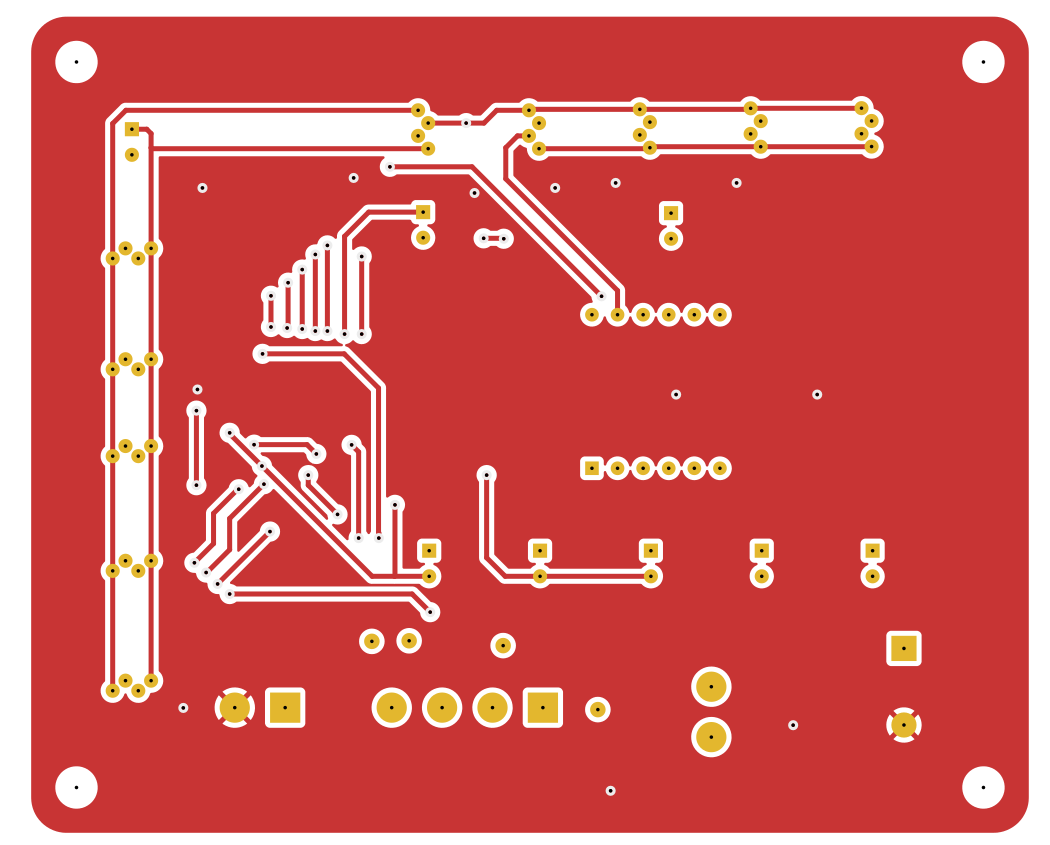
\includegraphics[width = 0.49\linewidth]{img/salt_ihm_tracks_front.png}
    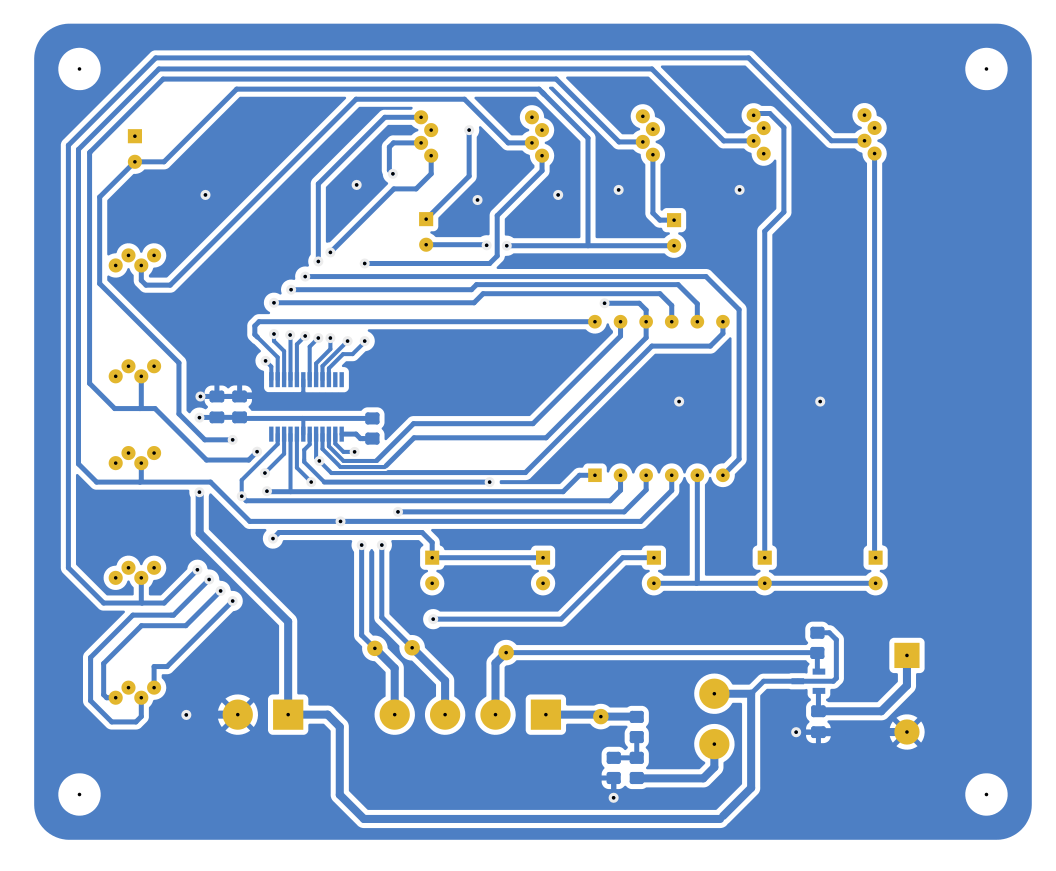
\includegraphics[width = 0.49\linewidth]{img/salt_ihm_tracks_back.png}
    \caption{Pistas y planos de la placa secundaria del SAL/T}
    \label{fig:salt_ihm_tracks}
\end{figure}    



Respecto al PCB (\textit{Printed Circuit Board}), se mandó a fabricar con la empresa JLCWAY \cite{jlcway} en China. Se utilizó el material FR-4, compuesto de fibra de vidrio y resina epoxi, para el substrato por su aislamiento eléctrico, su resistencia térmica y la relación entre rendimiento y costo lo que lo hace el estándar de la industria de PCBs. Ambas placas se fabricaron con 2 capas, la principal con dimensiones de 270mm x 260 mm mientras que la placa secundaria utilizada para el panel frontal mide 82mm x 100 mm. Se utilizó un grosor de placa de 1.6mm, placas de color verde con el \textit{silkscreen} (capa de serigrafía que contiene textos y símbolos impresos sobre la placa para identificar componentes, pines, y otras marcas importantes durante la fabricación y ensamblaje) de color blanco. En las figuras \ref{fig:salt_3d} y \ref{fig:salt_ihm_3d} se visualizan los modelos 3D de las placas diseñadas: 

\begin{figure}[H]
    \centering
    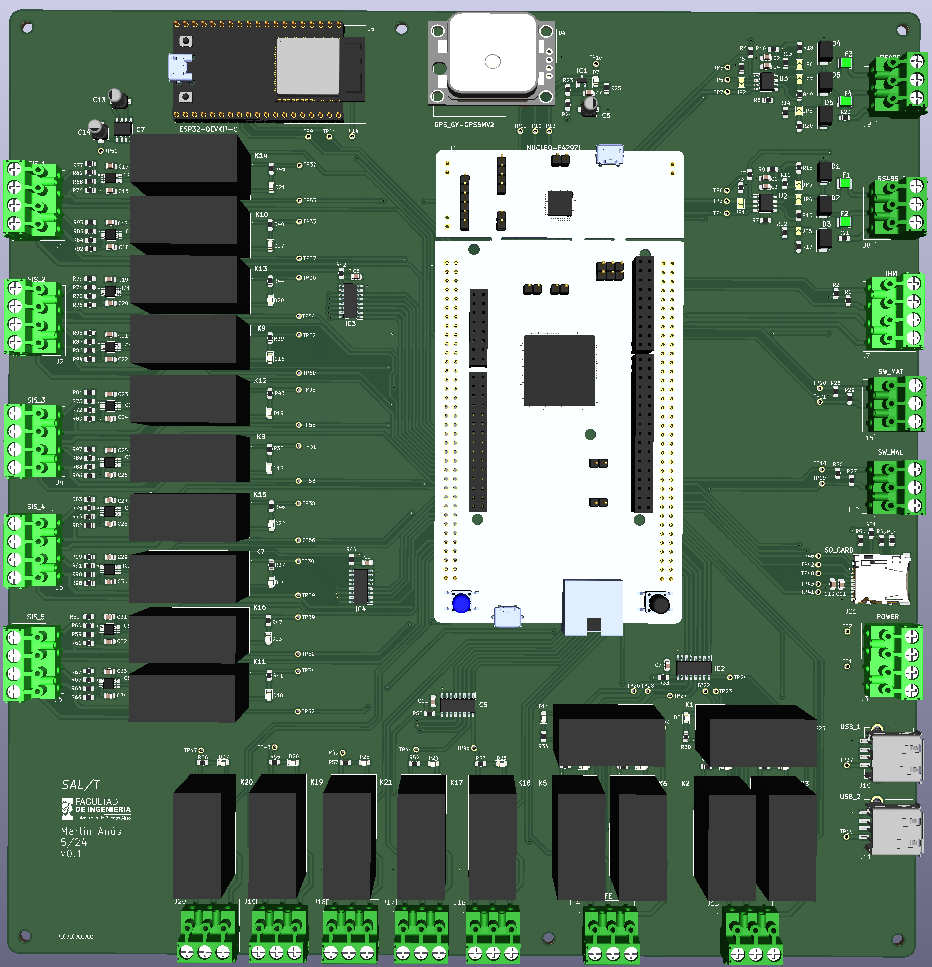
\includegraphics[width = \linewidth]{img/pcb_3d.png}
    \caption{Modelo 3D de la placa principal del SAL/T}
    \label{fig:salt_3d}
\end{figure}    



\begin{figure}[H]
    \centering
    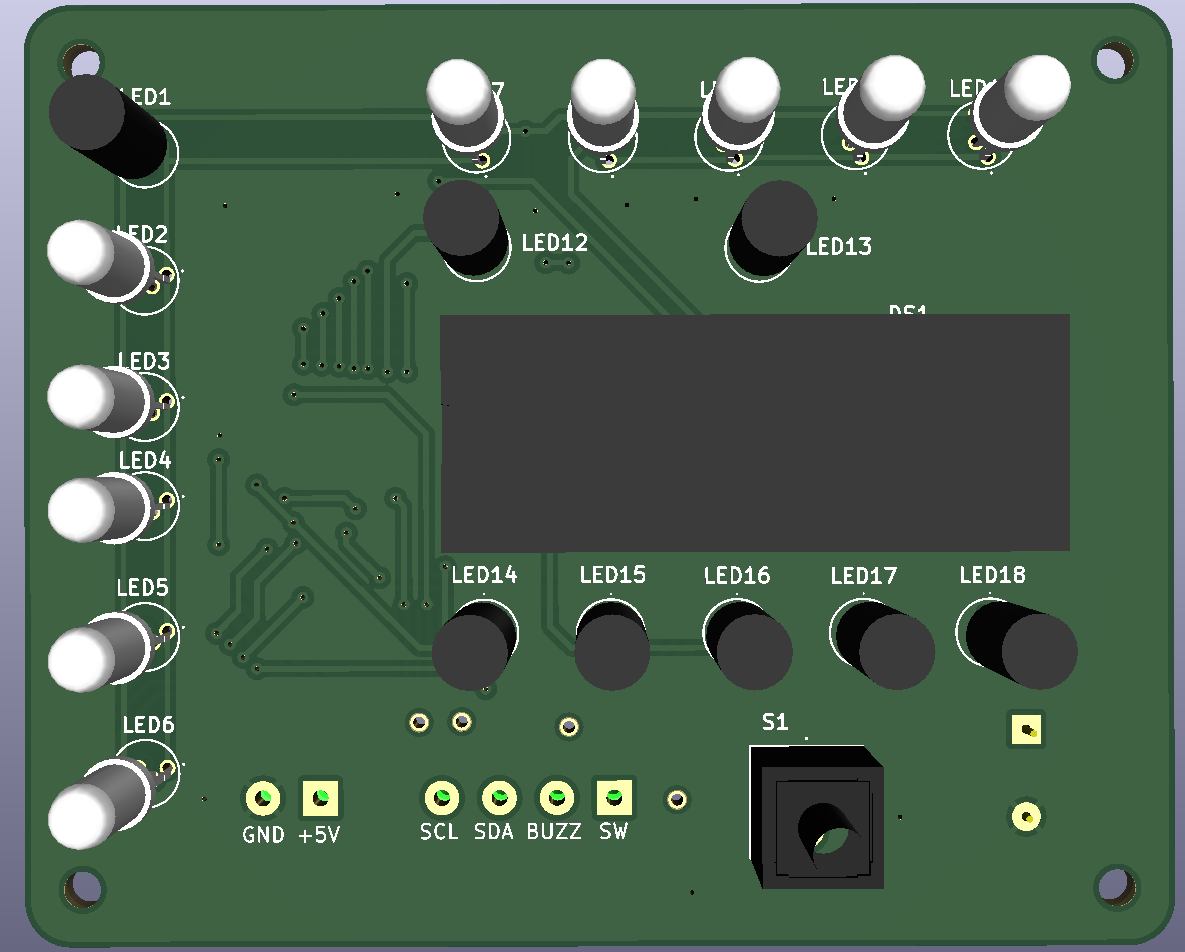
\includegraphics[width = 0.49\linewidth]{img/pcb_ihm_3d.png}
    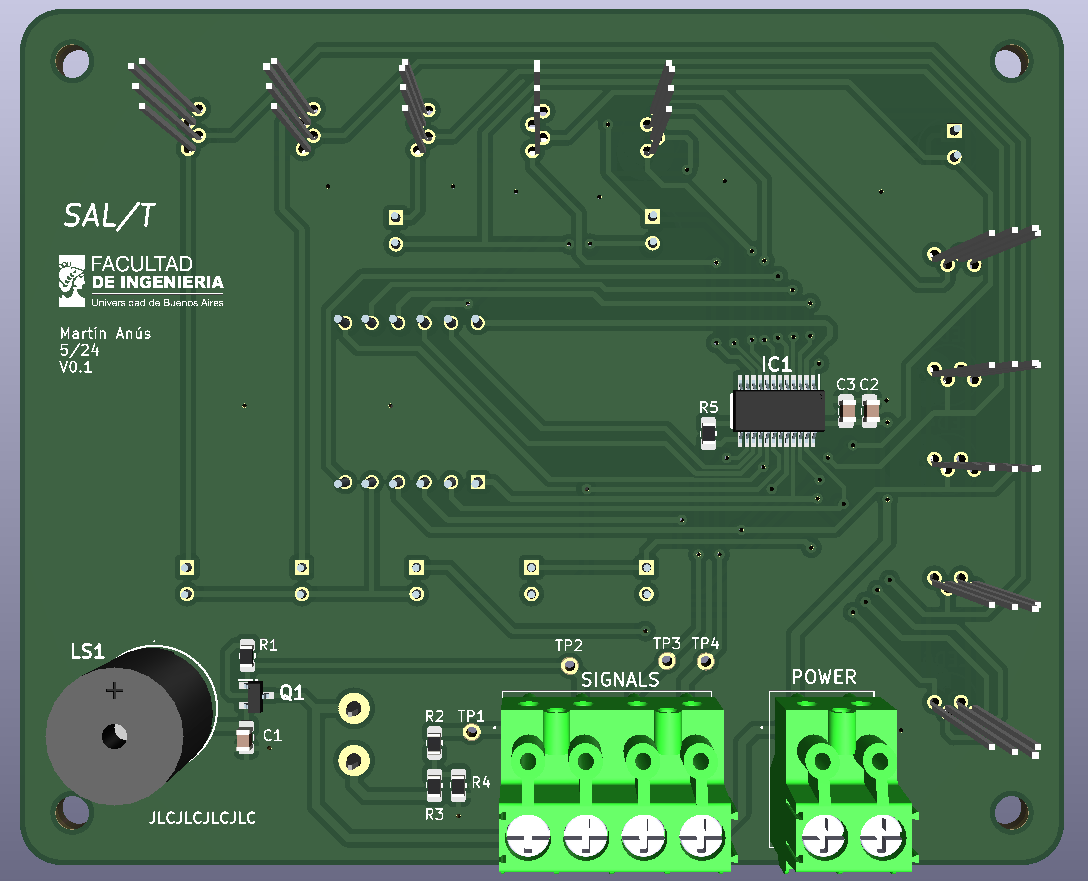
\includegraphics[width = 0.49\linewidth]{img/pcb_ihm_back_3d.png}
    \caption{Modelo 3D de la placa secundaria del SAL/T}
    \label{fig:salt_ihm_3d}
\end{figure}    




Los componentes fueron soldados a mano utilizando soldaduras de estaño. En las figuras \ref{fig:pcb_salt} y \ref{fig:pcb_salt_ihm} se visualiza la placa principal y la placa secundaria armada con todos los componentes montados. 

\begin{figure}[H]
    \centering
    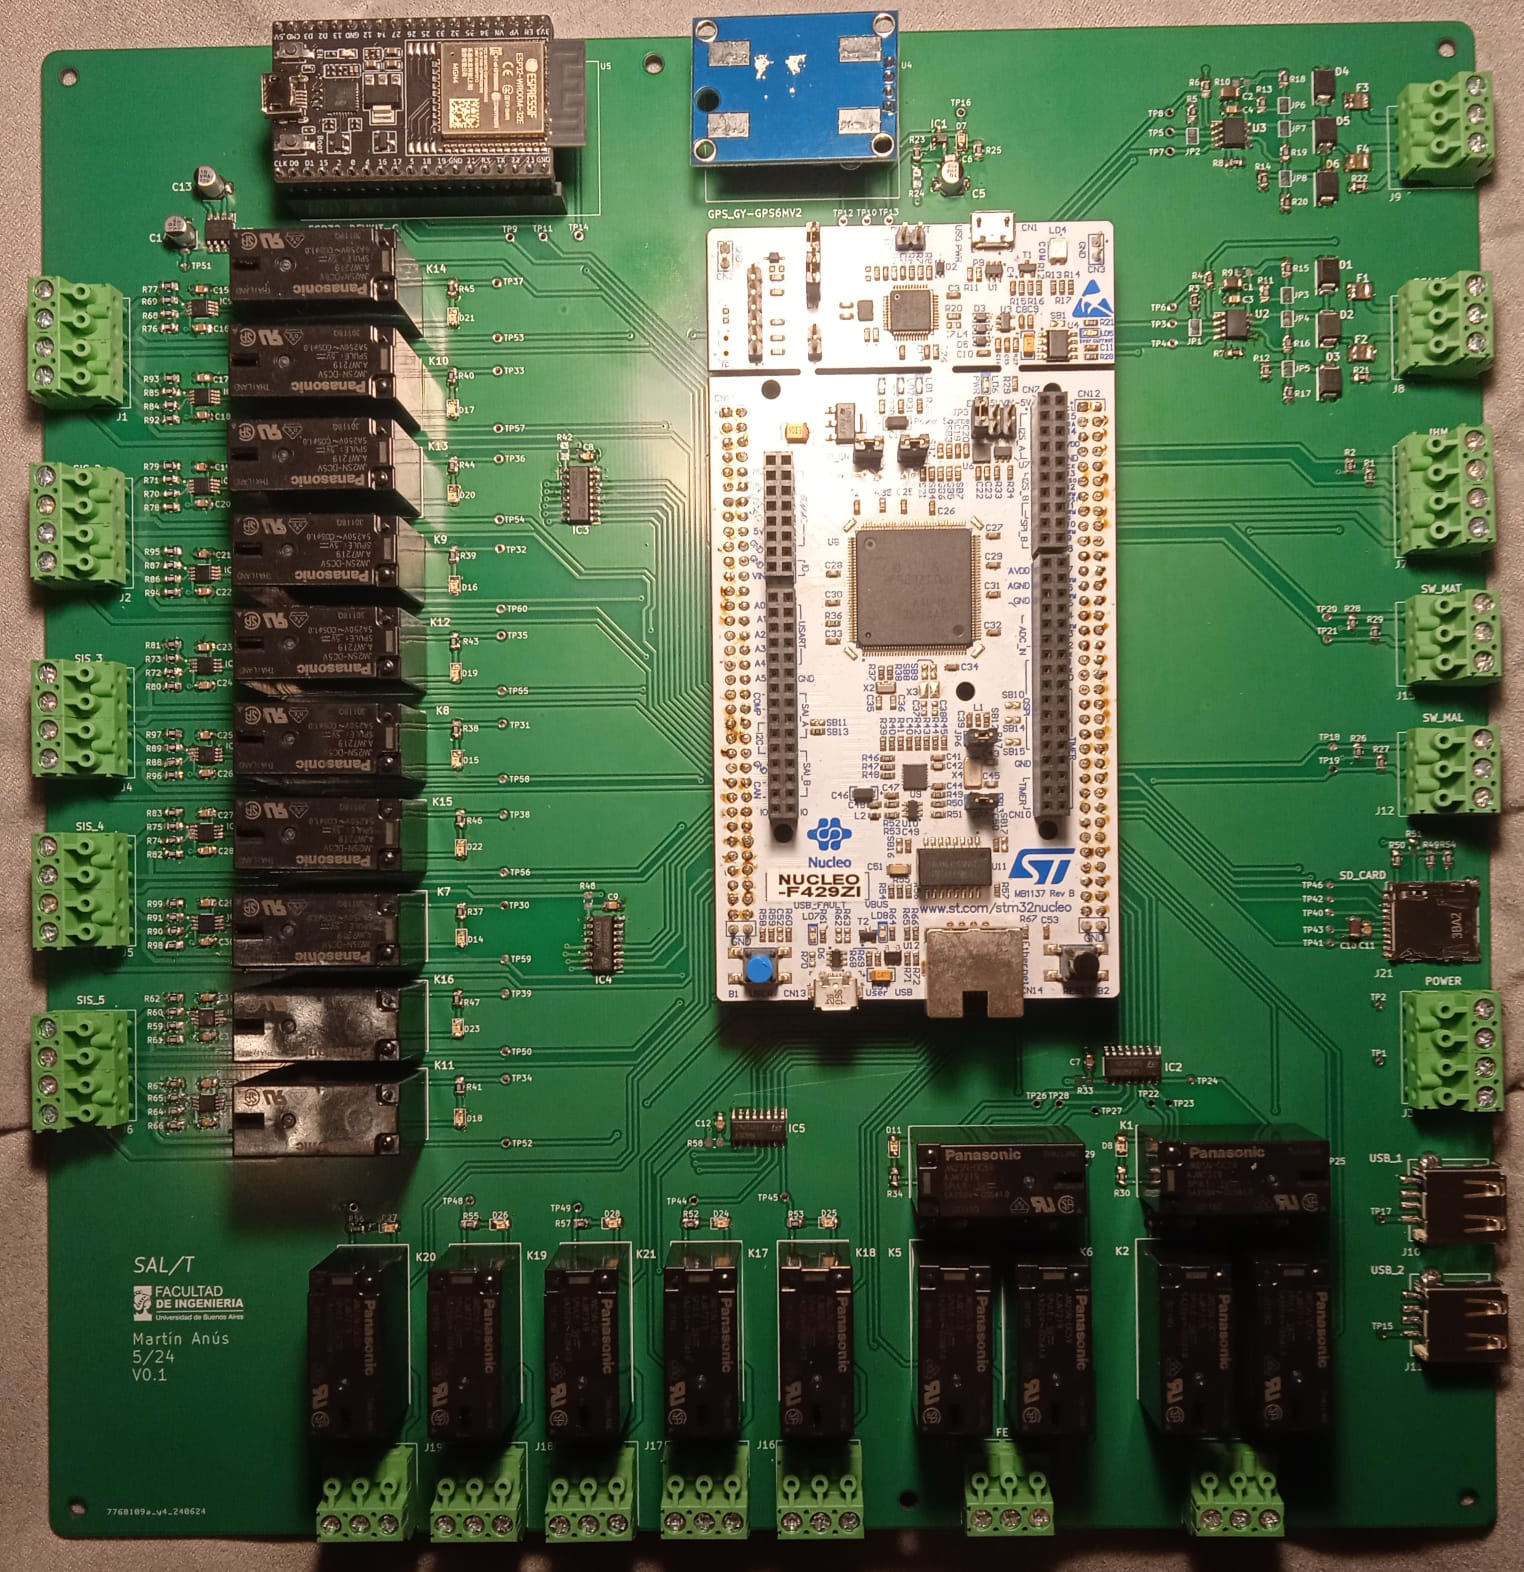
\includegraphics[width = \linewidth]{img/salt-placa_principal.jpeg}
    \caption{Placa principal del SAL/T fabricada}
    \label{fig:pcb_salt}
\end{figure}    



\begin{figure}[H]
    \centering
    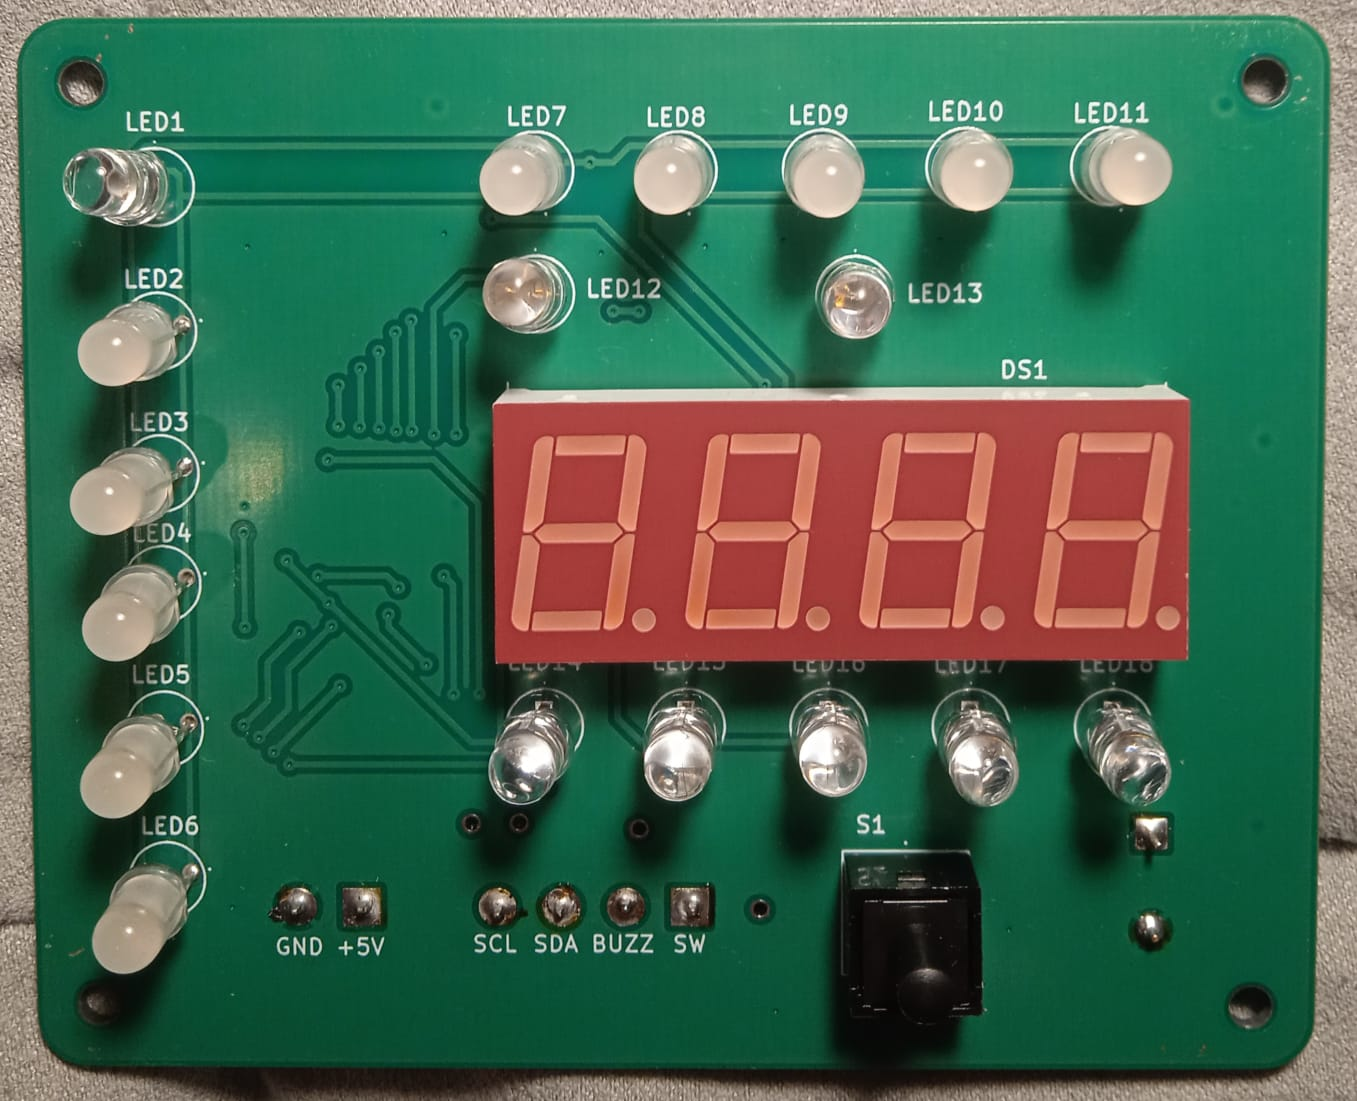
\includegraphics[width = 0.49\linewidth]{img/salt-placa_secundaria-front.jpeg}
    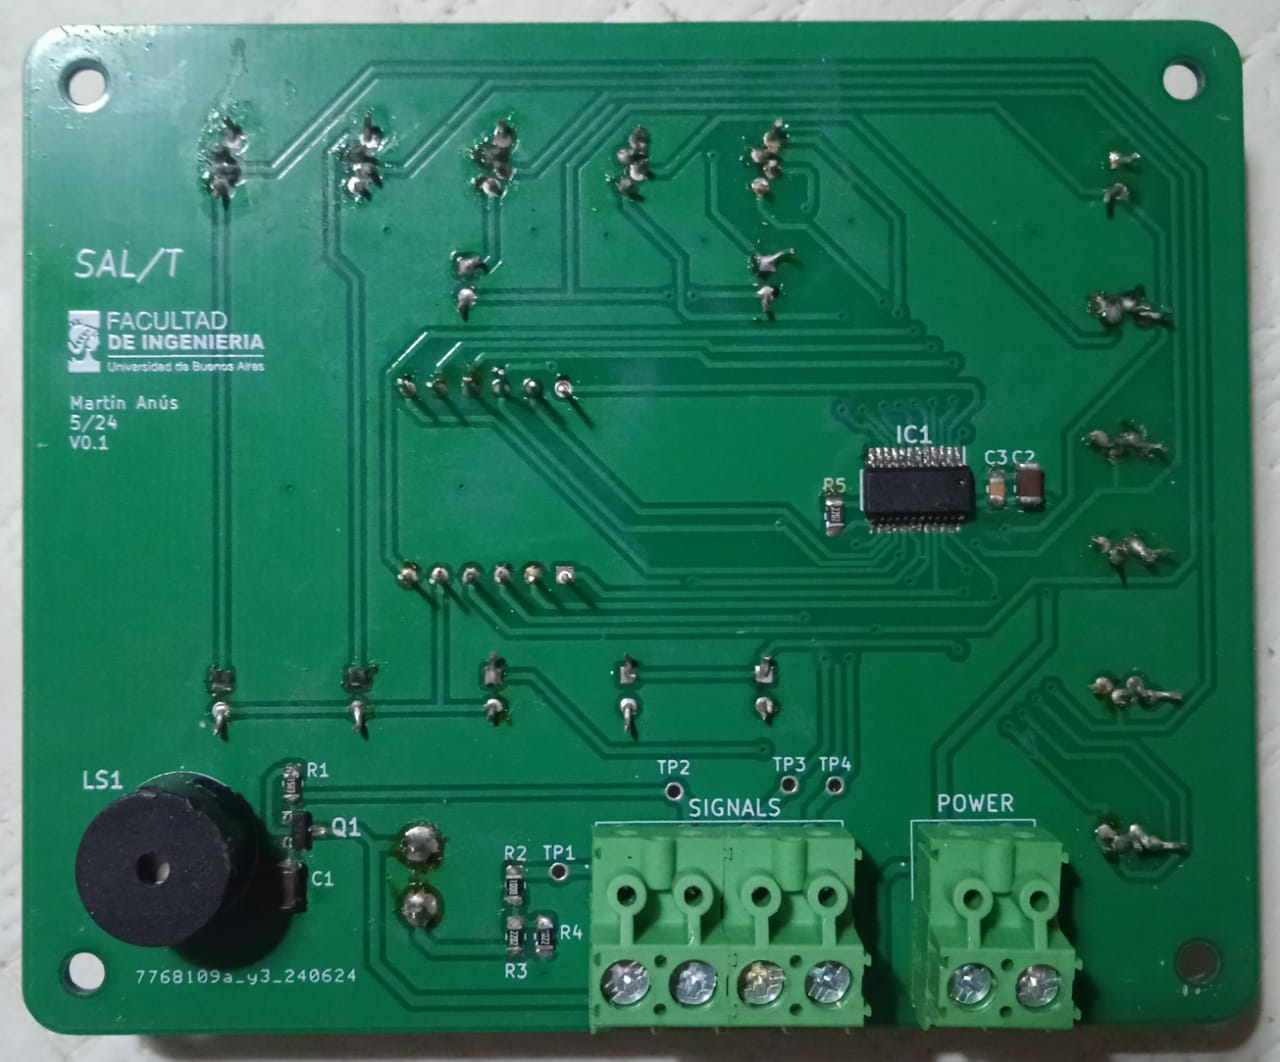
\includegraphics[width = 0.49\linewidth]{img/salt-placa_secundaria-back.jpeg}
    \caption{Placa secundaria del SAL/T fabricada}
    \label{fig:pcb_salt_ihm}
\end{figure}    
\subsubsection{Gabinete}

Una vez fabricadas y armadas las placas, se avanzó con el diseño de un gabinete para finalizar el diseño de hardware del prototipo. Considerando las medidas de las placas y que una de ellas funciona como parte del panel frontal del SAL/T, se realizó un diseño pensado para su fabricación en impresión 3D con medidas de 300 x 300 x 100mm. El panel frontal cuenta con los agujeros y espacios necesarios para que los LEDs, display y botones de la placa secundaria sean visibles por fuera. En la figura \ref{fig:gabinete_3d} se visualiza el diseño del gabinete.   

\begin{figure}[H]
    \centering
    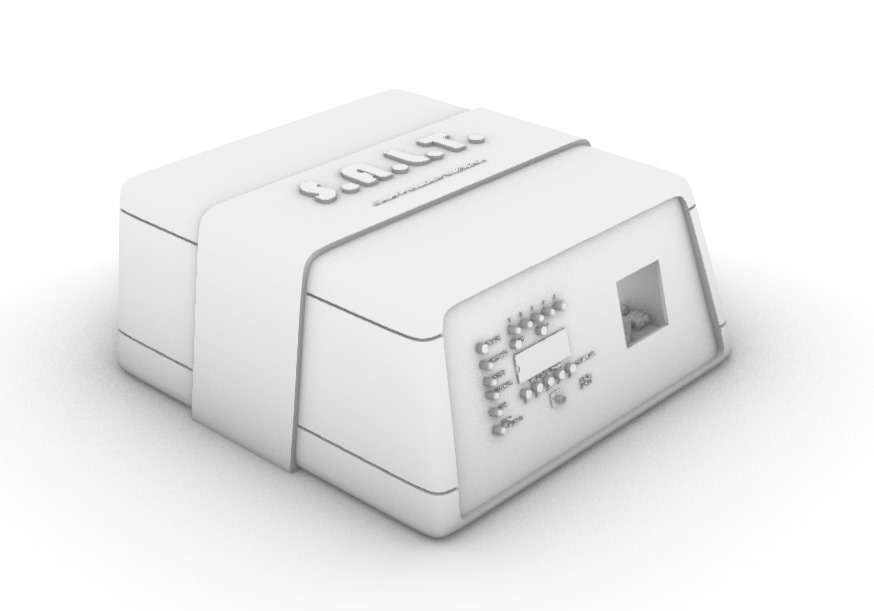
\includegraphics[width = \linewidth]{img/gabinete.jpeg}
    \caption{Diseño de gabinete para impresión 3D}
    \label{fig:gabinete_3d}
\end{figure}    

La fabricación del gabinete estaba pensada para realizarse utilizando la impresora 3D Prusa P3 Steel que tiene el Laboratorio Abierto (LABi) de la Facultad de Ingeniería de la Universidad de Buenos Aires \cite{labi_3d}. Considerando las dimensiones máximas que se pueden fabricar por pieza, se realizó la división del prototipo en 22 piezas que no excedan las dimensiones de 19 x 19cm. \\ 

Una vez finalizada la separación de las partes, se realizó la consulta con el LABi para su fabricación y, si bien el diseño y las piezas eran fabricables de manera individual, la fabricación del prototipo entero requería de demasiadas horas de uso de la impresora y demasiado material plástico debido a su gran tamaño y a la velocidad de fabricación del modelo de la impresora, lo que implicaba un costo innecesariamente alto para la fabricación del prototipo. \\ 

Por lo tanto, se siguieron las recomendaciones de utilizar un gabinete prefabricado para contener las placas del prototipo y realizar los ajustes necesarios para conseguir un panel frontal indicativo similar al diseñado previamente. Los gabinetes pensados para placas electrónicas son de menor dimensión, por lo que no se pudo conseguir ninguna para el prototipo. Finalmente, se consiguió un gabinete pensado para instalaciones eléctricas de 310 x 310 x 110mm con tapa atornillable que resultó ideal para el prototipo; el modelo es una caja estanca plástica blanca IP65 de Sistelectric, una empresa de Genrod \cite{gabinete}. El gabinete conseguido con las modificaciones realizadas se puede visualizar en la figura \ref{fig:gabinete_fabricado}. Las placas están atornilladas al gabinete y montadas sobre unos pequeños separadores para permitir que la placa no queda apoyada ni en contacto con el gabinete. 

\begin{figure}[H]
    \centering
    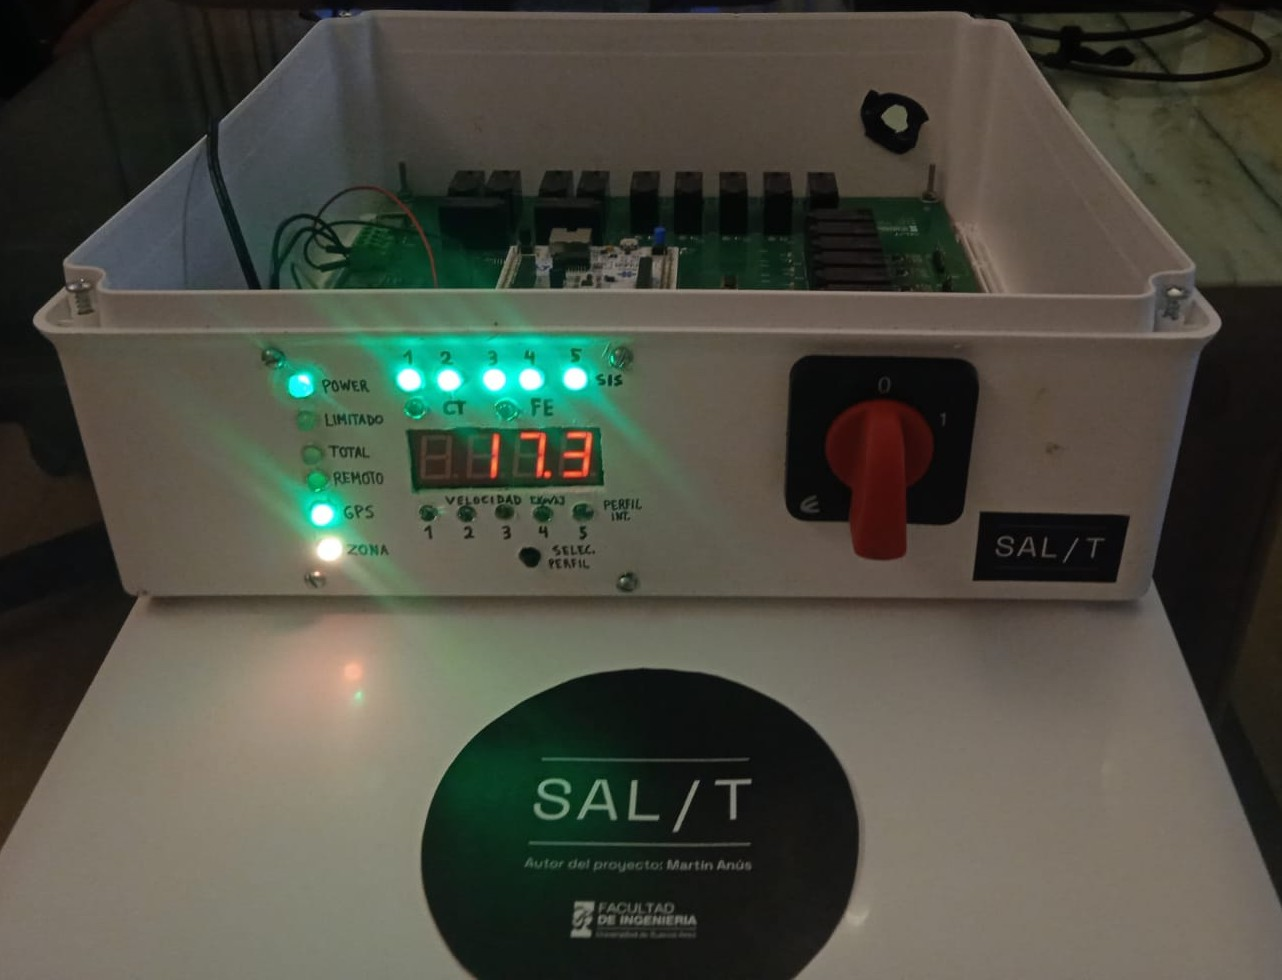
\includegraphics[width = \linewidth]{img/salt_fabricado.jpeg}
    \caption{Gabinete acondicionado para el prototipo del SAL/T}
    \label{fig:gabinete_fabricado}
\end{figure} 

Se realizaron las perforaciones necesarias para el panel frontal y la llave de activación. En la figura \ref{fig:frente_fabricado} se visualiza el frente del gabinete con la placa insertada y la llave de activación del modo aislado total. 

\begin{figure}[H]
    \centering
    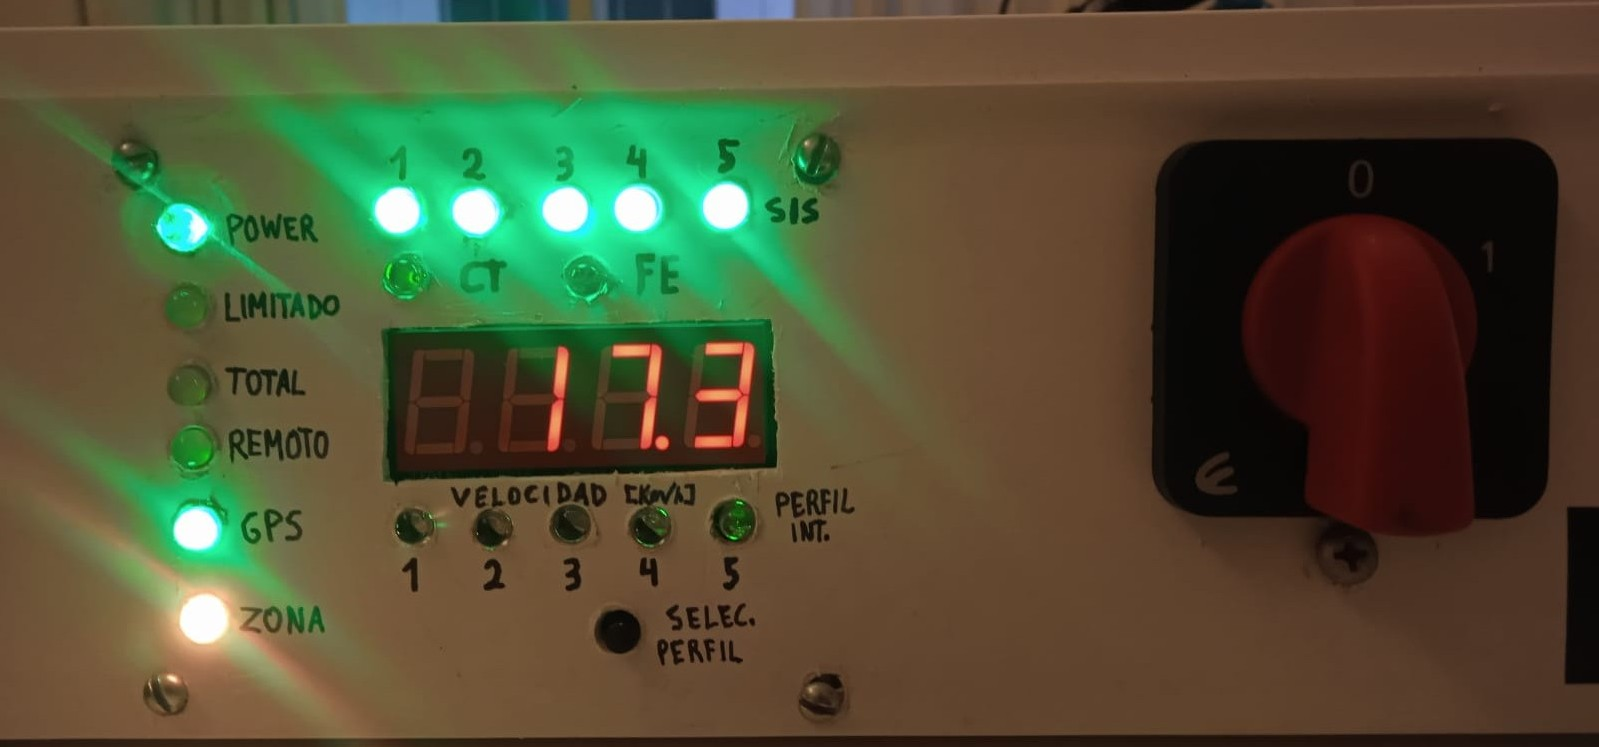
\includegraphics[width = \linewidth]{img/frente_fabricado.jpeg}
    \caption{Frente del del prototipo del SAL/T}
    \label{fig:frente_fabricado}
\end{figure} 

\subsection{Implementación de firmware}

\subsubsection{Lógica a nivel general}


El SAL/T resulta un sistema bastante complejo por la cantidad de entradas y variantes de comportamiento que considera para determinar su modo de operación y la activación de las señales críticas que resulta el componente de salida más relevante del sistema que le da propósito al SAL/T. La lógica de alto nivel que se puede considerar para el SAL/T se visualiza en la figura \ref{fig:logica_firmware}.  \\


Al comienzo, se inicializan todos los periféricos, las comunicaciones, los módulos y la memoria que forman parte del sistema. Por su lado, el ESP32 va a inicializarse y comunicarse con el servidor MQTT a través de alguna de las redes Wi-Fi que tenga configurado, para suscribirse a la recepción de comandos y poder reportar el estado y registro de eventos del sistema de manera remota. \\

Luego, se leen las entradas del sistema. Por un lado, el sistema lee el estado de las llaves de activación de modo aislado limitado y total, y los comandos remotos para determinar el modo de operación del SAL/T. Por otro lado, se leen las entradas del estado de los SIS, la ubicación GPS, la velocidad que puede ser obtenida por cualquiera de sus fuentes de medición siguiendo la prioridad de Hasler Tesloc 1500, luego el generador de impulsos ópticos y luego la señal GPS. \\ 

Una vez que el sistema tiene el dato de todas las entradas, va a mostrar a través del panel frontal y registrar a través del almacenamiento interno y remoto, cualquier estado o cambio relevante del sistema. \\ 

Luego, se determina cuál debe ser el modo de operación del SAL/T basado en el primer grupo de entradas mencionado, y se activan las rutinas de entrada en cada modo. \\

Finalmente, con el modo de operación ya configurado y el resto de las entradas, se determina los valores que deben tomar las salidas de señales críticas como el corte de tracción, freno de emergencia o bypass de los SIS. Al finalizar, se vuelve al comienzo de lectura de entradas y se mantiene funcionando esta lógica de manera general en todo momento. 


\begin{figure}[H]
    \centering
    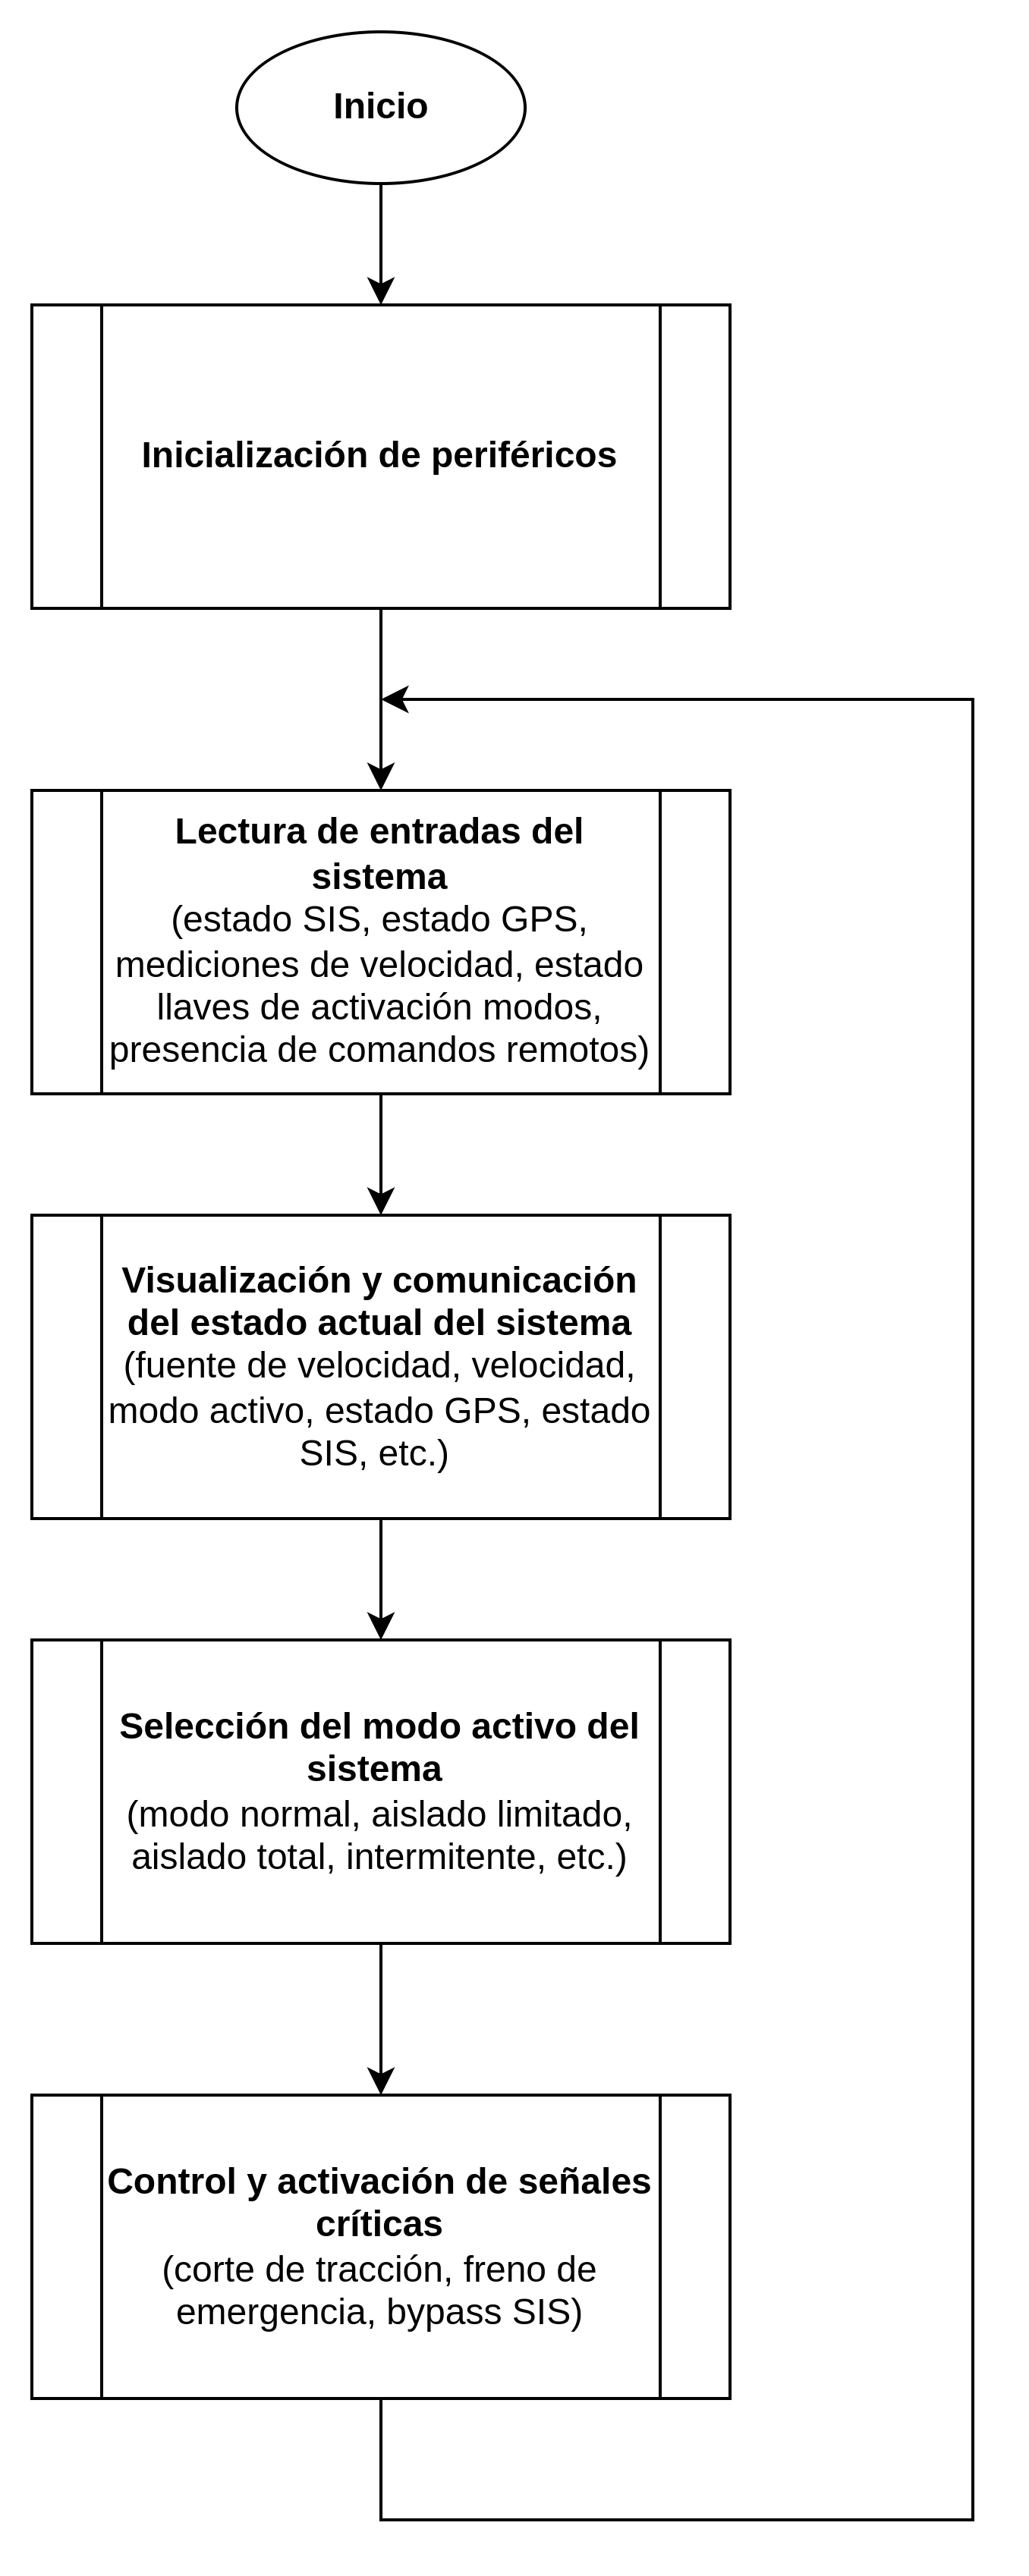
\includegraphics[scale = 0.6]{img/logica_firmware.png}    
    \caption{Lógica general del firmware del SAL/T}
    \label{fig:logica_firmware}
\end{figure}    




En la figura \ref{fig:modos_salt} se visualiza un diagrama con la lectura de los comandos más relevantes y llaves de activación local que participan de la selección del modo de operación y dentro de cada modo el estado general de las señales críticas. 


\begin{figure}[H]
    \centering
    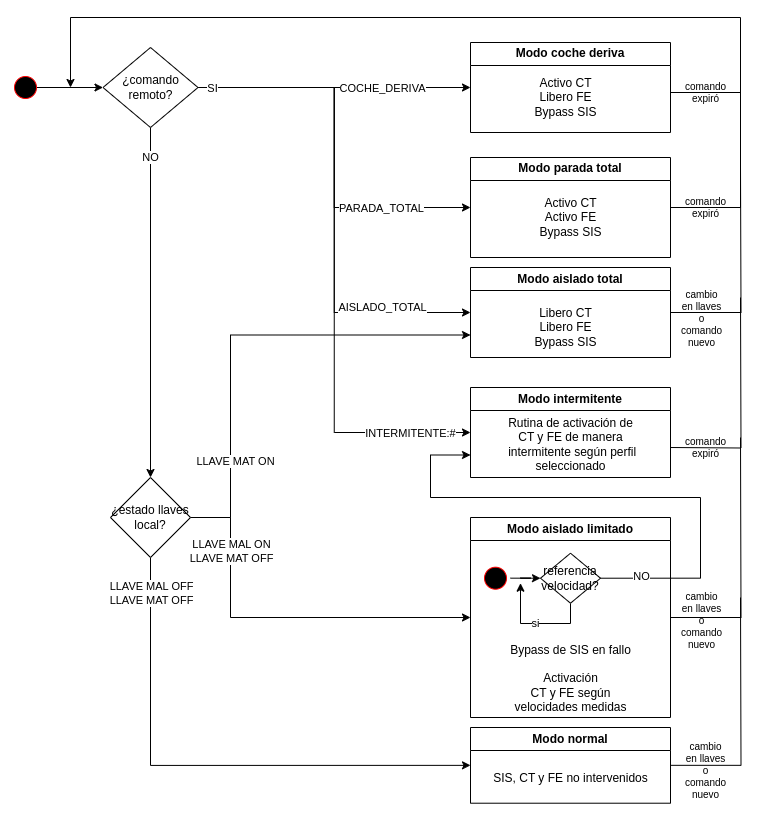
\includegraphics[width = \linewidth]{img/modos_salt.png}    
    \caption{Diagrama de flujo de modos de operación del SAL/T}
    \label{fig:modos_salt}
\end{figure}    

\subsubsection{Mecanismos de RTOS}

El firmware del SAL/T está implementado utilizando FreeRTOS \cite{freertos} para permitir una ejecución pseudo-concurrente de las distintas tareas de manera eficiente, mejorando la respuesta del sistema ante eventos y mejorando el manejo de sus recursos. Se obtiene mayor control sobre la prioridad de las tareas y tiempos de respuesta, lo que lo hace ideal para aplicaciones de tiempo real críticas. Además, facilita la integración de sistemas complejos a través de las funcionalidades de asignación de tareas, comunicación entre tareas y manejo de memoria, siendo a la vez ligero y altamente personalizable para entornos de hardware específicos. \\ 


Se utilizó la interfaz de FreeRTOS-CMSIS versión 1.02, configurado con la unidad de punto flotante habilitada, permitiendo que las tareas de mayor prioridad interrumpan a las de menor prioridad (\textit{preemption}), asignando 15360 bytes de memoria para el tamaño total del \textit{heap}. \\

Las distintas \textit{tasks} o tareas utilizadas en el sistema son las siguientes: 

\begin{itemize}
    \item \textbf{commsTask - prioridad alta}: Esta tarea se encarga de procesar los mensajes recibidos por cualquiera de las comunicaciones con dispositivos externos. Su prioridad es alta porque estas comunicaciones pueden traer datos que modifiquen completamente el estado del sistema y deben ser considerados lo antes posible para corregir el estado del sistema. 
    \item \textbf{systemTask - prioridad media}: Esta tarea se encarga de leer de manera sistemática las entradas disponibles del sistema y luego de visualizarlas y registrarlas. 
    \item \textbf{modeTransTask - prioridad media}: Esta tarea va a utilizar los últimos datos de entrada recibidos para determinar el modo de operación en el que se debe ejecutar el sistema.
    \item \textbf{criticalSigTask - prioridad media}: Esta tarea se encarga de, basado en el modo de operación activo y en las demás entradas del sistema, determinar la activación o liberación de las señales críticas del sistema. 
    \item \textbf{reportTask - prioridad baja}: Esta tarea reporta de manera periódica el estado del sistema de manera remota. Su prioridad es la más baja porque no modifica el comportamiento real del sistema y resulta no crítico el desfasaje en la trasmisión. 
\end{itemize}


Las tareas de prioridad media ejecutan su rutina, y al terminar se pone un delay del sistema operativo de 500ms y se le devuelve el control al \textit{scheduler} para que asigne los recursos de procesamiento a la tarea que siga en la cola de prioridades establecida. A ese delay se le suma una baja cantidad aleatoria de milisegundos para evitar la posible sincronización de las tareas. Por otro lado, la tarea de prioridad baja se ejecuta de manera periódica cada un tiempo configurable, por defecto 5 segundos. Las rutinas de todas las tareas se finalizan de manera rápida en pocos milisegundos permitiendo que el asignador de tareas le dé el procesamiento a todas las tareas mientras se cumple el delay configurado para cada uno; de esta manera se evita lo que se conoce como \textit{starving} (que las tareas de menor prioridad nunca se ejecuten). \\ 

En cuanto a la tarea de mayor prioridad, se utilizó otro mecanismo de sincronización de FreeRTOS para facilitar el procesamiento de las comunicaciones; se utilizó un semáforo binario. Este mecanismo de sincronización tiene dos estados, disponible (1) o no disponible (0). Se utiliza para gestionar el acceso a un recurso compartido o para sincronizar tareas e interrupciones. Una tarea da o libera el semáforo cuando un evento ocurre, y otra tarea lo toma cuando está disponible; permitiendo la ejecución controlada de procesos dependientes. \\

En el SAL/T, todas las comunicaciones con sistemas externos (módulo GPS, módulo Wi-Fi, fuentes de medición de velocidad, conexión serie local) están conectados por interfaz UART al MCU y tienen habilitada la recepción por interrupción. Esta interrupción por hardware tiene mayor prioridad que las tareas del kernel lo que permite interrumpir cualquier tarea que se esté ejecutando. En la función de \textit{callback}, se mantienen buffers de recepción separados (uno por interfaz), hasta detectar la recepción de una línea completa de un mensaje. En ese momento, se almacena la línea completa en una variable global, accesible desde la rutina de las comunicaciones, y se libera el semáforo de comunicaciones. \\

Al terminar la interrupción por hardware, el asignador de tareas reprioriza las tareas y en caso de haber liberado el semáforo, le pasa el control a la tarea de mayor prioridad. En esta tarea se verifica qué comunicación tiene un mensaje nuevo y allí se procesan los datos correspondientes. Al finalizar, se vuelve a tomar el semáforo bloqueando la tarea hasta la recepción de una nueva línea de información. 

 
\subsubsection{Medición del estado de los SIS}


La medición del estado de los distintas señales de los SIS se realiza utilizando el conversor analógico digital (ADC) que trae el MCU; este permite la conversión de señales analógicas valores digitales que pueden ser procesados por el microcontrolador. En este caso, se utiliza el ADC3 del STM32, configurado para realizar conversiones en 10 canales diferentes. \\

La configuración del ADC se realizó para que opere con una resolución de 12 bits, lo que proporciona un rango de valores digitales de 0 a 4095, permitiendo una representación precisa de las señales analógicas; para lograr esta resolución, se consumen 15 ciclos del reloj de ADC. El prescaler del reloj se ajustó con un divisor de 8 lo que determina una operación a 10,5 MHz, y el modo de conversión en escaneo está habilitado para permitir la lectura de múltiples canales de manera secuencial. \\ 

El ADC está configurado para iniciar las conversiones mediante software, sin utilizar un disparador externo, lo que otorga mayor control sobre el inicio de las conversiones. Las conversiones no son continuas, y el DMA (Acceso Directo a Memoria) está deshabilitado de manera continua, permitiendo un mayor control del flujo de datos en el sistema. Además, los resultados se alinean a la derecha, lo que permite un procesamiento eficiente de los datos en 12 bits. \\

Se declara una función de callback HAL\_ADC\_ConvCpltCallback que se ejecuta al finalizar la 10ma conversión del ADC. En esta, se prende un flag de que hay una serie de valores medidos y se reinicia el proceso de adquisición de datos mediante DMA en los 10 canales configurados. El DMA permite que los datos del ADC se transfieran directamente a la memoria sin la intervención del procesador, lo que reduce la carga de la CPU y mejora el rendimiento. En modo no continuo, el ADC realiza conversiones de datos de manera intermitente o bajo demanda, activando el DMA solo cuando es necesario transferir una nueva muestra. \\

Cuando se corre la rutina de lectura de entradas del sistema, se verifica si hay una nueva serie de valores medidos. En ese caso, se compara para cada uno de los canales medidos (5 señales de CT y 5 de FE, una para cada SIS) con un valor umbral configurado dependiendo la tensión con la que trabaje el tren. Conociendo el circuito de hardware que reduce la tensión al rango de los 3,3 V y sabiendo cuál es la tensión esperada en una llave abierta, se puede determinar qué valor es esperable encontrar en el ADC para una llave abierta. Para una llave cerrada, la tensión en sus terminales es cero y el valor que arroja el ADC también es cercano a 0. Por lo tanto, utilizando un umbral cercano al valor medio entre 0 y el esperado cuando la llave esté abierta, se puede determinar con el mejor margen el estado real de las señales del SIS. 
\subsubsection{Interacción con datos GPS}

El módulo GPS utilizado en el sistema se comunica mediante interfaz UART con el MCU del sistema. Se configuró la UART5 para esta comunicación, con un \textit{baudrate} de 9600, una longitud de palabra de 8 bits, sin bit de paridad y un bit de parada conocido como configuración 8N1. No se emplea control de flujo por hardware y el sobremuestreo está configurado en 16, lo que mejora la precisión en la recepción de datos. \\ 

El módulo GPS transmite datos a una frecuencia de 1 Hz, es decir, una vez por segundo, enviando múltiples líneas de información conocidas como frases NMEA (\textit{National Marine Electronics Association}). Estas sentencias incluyen detalles sobre la posición (latitud y longitud), velocidad, altitud, fecha, hora y estado de los satélites \cite{nmea}. En este proyecto, se utiliza la línea de GPRMC (\textit{Recommended minimum specific GPS/Transit data}); una de las más importantes en la transmisión de datos GPS. Contiene información esencial como la hora, fecha, posición (latitud y longitud), velocidad sobre el suelo y dirección y es utilizada para obtener los datos mínimos necesarios para la navegación. \\ 

La recepción de la información se realiza utilizando la comunicación por interrupción donde un \textit{buffer} receptor permite identificar el comienzo de esta frase porque siempre comienza por los caracteres \$GPRMC y termina por el carácter de retorno de línea. Una vez leída una línea completa, se activa el semáforo de procesamiento de comunicaciones y una vez terminada la interrupción de hardware de la UART, el RTOS va a priorizar el procesamiento de esta línea. Se almacena una marca de tiempo de la recepción de este dato para más adelante poder verificar la validez o expiración de la información si no se recibieron nuevos datos. La línea trae definida el orden de los datos incluidos separados por una coma. De esta manera, se generó un \textit{parser} que permite asignar a una estructura los distintos datos presentes en la frase GPRMC. \\ 

El dato más relevante a consultar es el estado de la trasmisión. Si este dato indica que la conexión está ausente (probablemente por falta de señal de la antena con los satélites), todos los otros datos deben ser descartados. En caso de leer un estado de conexión exitoso, se determinan los datos de latitud, longitud, y velocidad transmitidos por el módulo. \\

\subsubsection{Procesamiento de velocidades por RS-485}

Para la comunicación con las fuentes externas de medición de velocidad, se utilizaron las interfaces UART7 y UART8 del MCU que, a través de un circuito conversor de UART a RS-485, logra comunicarse con los sistemas externos. La configuración de ambos UART establece la comunicación serie con una velocidad de 115.200 baudios, utilizando 8 bits de datos, 1 bit de parada y sin paridad. El modo está configurado sin control de flujo por hardware, y con sobremuestreo a 16, lo que asegura una comunicación eficiente y precisa. \\

La interfaz RS-485 1, conectada con la señal interceptada entre el Hasler Teloc 1500 y el indicador de velocidad de la formación, recibe el dato de la velocidad encapsulado dentro de un paquete de 31 bytes. Este paquete comienza y termina siempre por el byte 0x7E lo que permite delimitar la trama. Esta interfaz trabaja con la recepción por interrupción y al detectar el byte de inicio comienza almacenar la información recibida y al recibir el byte de stop, validando una longitud de 31 bytes totales, termina la línea de datos. En ese momento, se libera el semáforo para que el RTOS permita la ejecución de la rutina de procesamiento de esta línea donde se extrae de los bytes 7 y 8 la información de la velocidad. Nuevamente se incluye una marca de tiempo para verificar la validez del dato antes de ser utilizado en otras rutinas. \\

La interfaz RS-485 2, conectada con la medición de velocidad proveniente del generador de impulsos ópticos, recibe el dato de la velocidad de manera directa. Se espera la recepción de un mensaje numérico seguido de un carácter de retorno de línea. Esta interfaz, conectada al UART8, funciona utilizando la recepción por interrupción y mediante un \textit{buffer} que almacena cada carácter hasta encontrar la finalización de la línea. Una vez completa la línea, se activa el semáforo para que al finalizar la rutina de interrupción, el RTOS pueda darle mayor prioridad al procesamiento de esa línea donde se va a intentar convertir los caracteres leídos a un valor numérico y almacenarlo como dato de velocidad. También se almacena una marca de tiempo para asociarla al dato de velocidad y permitir la expiración de este dato tras algunos segundos sin recepción de nuevos valores. 
\subsubsection{Comunicación con central operativa}

La comunicación del SAL/T con la central operativa se va a realizar a través del módulo ESP32 que permite la conectividad Wi-Fi utilizando el protocolo MQTT para el intercambio de mensajes. \\

El módulo ESP32 se conecta el MCU utilizando la interfaz UART4 con una configuración 8N1 con un \textit{baudrate} de 115.000 y sobremuestreo de 16 veces. Esta comunicación va a ser de manera bidireccional, ya que ambos dispositivos van a trasmitir y recibir datos. El ESP32 está configurado para hacer principalmente de puente entre el MCU y el broker MQTT; esto significa que cualquier mensaje que reciba del MCU, lo va a retransmitir al MQTT y cualquier mensaje que recibe de MQTT lo va a retransmitir al MCU. También tiene la funcionalidad de mantener la fecha y hora del SAL/T actualizado ante un eventual corte en la alimentación consultando un cliente NTP (Network Time Protocol) para obtener la hora actual de un servidor en Internet.\\ 

El ESP32 permite la configuración de los datos de hasta 2 redes Wi-Fi y constantemente va a estar verificando la conexión y, en caso de desconexión, intentando conectarse de manera alternada a cualquiera de ellas. Una vez conectado a una red Wi-Fi, se va a registrar en el broker MQTT configurado donde va a suscribir al \textit{topic} salt\_remote\_command. En este \textit{topic}, la central operativa va a publicar los comandos a aplicar sobre el SAL/T por lo que cualquier mensaje recibido, va a ser enviado al MCU para su procesamiento. Además, cada 10 segundos el módulo va a consultar el servidor NTP pool.ntp.org \cite{ntp} para obtener la fecha y hora exacta y transmitírsela al SAL/T. \\ 

En sentido inverso, el ESP32 está constantemente levantando cualquier mensaje que pueda recibir por la interfaz UART. Al recibir un mensaje (terminado por un retorno de línea), el módulo va a leer los primeros caracteres (contando hasta un carácter delimitador) para determinar a qué \textit{topic} MQTT corresponde enviar el mensaje siguiendo la tabla \ref{tab:mqtt_topics}.

\begin{table}[H]
    \centering
    \begin{tabular}{|c|c|}
        \hline
         \textbf{Comienzo mensaje} & \textbf{\textit{Topic}}  \\ \hline
         LOG & salt\_remote\_log  \\ \hline
         ACK & salt\_remote\_ack  \\ \hline
         STATUS  & salt\_status  \\          
         \hline
    \end{tabular}
    \caption{Identificación de \textit{topic} MQTT}
    \label{tab:mqtt_topics}
\end{table}



En la figura \ref{fig:mqtt_bloque} se visualiza un diagrama de la comunicación entre el SAL/T y la central operativa con las distintas partes involucradas previamente explicadas. 

\begin{figure}[H]
    \centering
    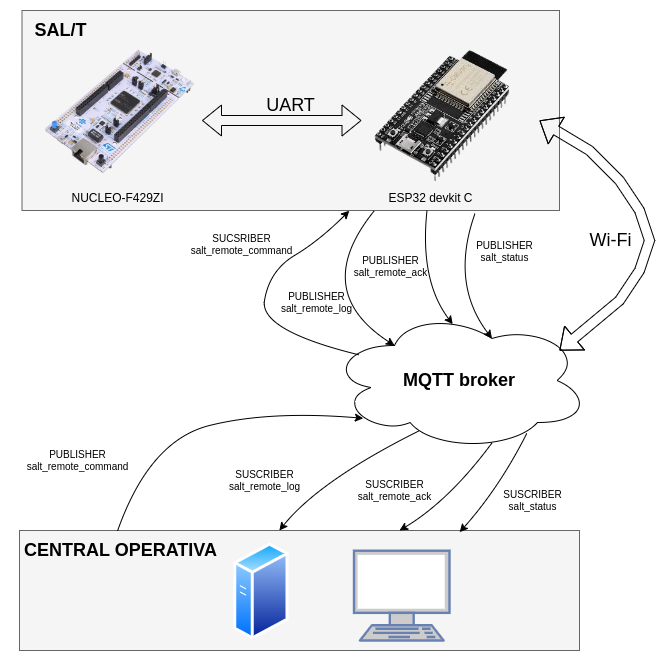
\includegraphics[width = \linewidth]{img/mqtt_bloques.png}    
    \caption{Diagrama de la comunicación entre el SAL/T y la central operativa}
    \label{fig:mqtt_bloque}
\end{figure}    




El \textit{topic} salt\_remote\_status se utiliza para que el SAL/T reporte su estado de manera periódica independientemente de los cambios que puedan ocurrir en el sistema. Por defecto, se reporta el estado general del sistema cada 5 segundos siendo este tiempo un parámetro configurable del sistema. En este mensaje, se reporta el modo que esté activo en el SAL/T. El \textit{topic} salt\_remote\_log se utiliza para transmitir todos los cambios de estado del sistema y permitir guardar un registro de eventos en la central operativa en tiempo real. \\


Los \textit{topics} salt\_remote\_commands y salt\_remote\_ack se utilizan para el envío de comandos y confirmación de recepción entre la central operativa y el SAL/T. Los comandos enviados tienen una estructura de ID|COMANDO:PARÁMETROS que permite luego al sistema separar los distintos datos. De recibir y procesar correctamente el comando, el SAL/T va a responder por el \textit{topic} salt\_remote\_ack un mensaje con el formato ACK:ID utilizando el mismo ID recibido en el comando para confirmarle a la central operativa la recepción y ejecución del comando enviado. Los comandos que modifican el estado del SAL/T de manera continua, tienen un tiempo de validez configurable, por defecto de 10 segundos, que una vez transcurrido son considerados inválidos. \\ 



A continuación se detallan los distintos comandos aceptados por el SAL/T y una breve explicación del comportamiento del sistema al recibirlos. 

\begin{itemize}
    \item \textbf{AISLADO\_TOTAL}: Este comando fuerza el estado del SAL/T al modo aislado total donde todos los SIS son aislados y se liberan las señales de CT y FE. 
    
    \item \textbf{PARADA\_TOTAL}: Este comando fuerza la activación de las señales de CT y FE del SAL/T llevando la formación a un estado de detención forzosa. 
    
    \item \textbf{COCHE\_DERIVA}: Este comando fuerza la activación de la señal de corte de tracción, pero libera la señal de freno de emergencia aislando cualquier SIS que pueda estar activando la señal. 
    
    \item \textbf{INTERMITENTE:int}: Este comando recibe un comando numérico del 1 al 5 que indica el perfil intermitente que se debe activar. El SAL/T pasa a estado intermitente siguiendo los tiempos de aceleración, desaceleración y freno configurados para el perfil seleccionado. 

    \item \textbf{CANCEL}: Este comando cancela cualquier otro comando que esté vigente en el SAL/T. 
    
    \item \textbf{REPORT\_STATUS\_PERIOD\_CONFIG:int}: El parámetro corresponde a la cantidad de segundos que se desea configurar como período de trasmisión de reporte de estado del SAL/T. Por defecto son 5 segundos pero se acepta la modificación en un rango de 1 a 60s. 
    
    \item \textbf{COMMAND\_VALIDITY\_CONFIG:int}: El parámetro corresponde a la cantidad de segundos que se desea configurar como tiempo de validez de un comando remoto activo. Por defecto son 10 segundos, pero se acepta la modificación en un rango de 1 a 60s. 
    
    \item \textbf{SPEED\_CONFIG:int,int,int,int,int}: Se configura uno de los perfiles de velocidades que controlan la formación en el modo aislado limitado. El primer parámetro corresponde al perfil a configurar (valor entre 0 y 3 que corresponde a la zona de circulación 1, 2 y 3 y cuando no hay referencia de ubicación), luego los otros 4 parámetros corresponden a la velocidad límite para desacelerar, la velocidad límite para volver a acelerar en caso de activación del CT, la velocidad límite para aplicar el freno de emergencia y el tiempo mínimo de frenado una vez superado el umbral anterior. 
    
    \item \textbf{INTERMITENTE\_CONFIG:int,int,int,int,int}: Se configura uno de los perfiles que controla la formación en modo intermitente. El primer parámetro corresponde al perfil a configurar (valor entre 1 y 5), luego los otros 4 parámetros corresponden el tiempo de aceleración por ciclo, el tiempo de desaceleración por ciclo, la cantidad de ciclos antes de aplicar el freno, y el tiempo de frenado luego de transcurridos los ciclos configurados. 
    
    \item \textbf{DOWNLOAD\_LOGS}: Este comando permite extraer toda la información de registro de eventos que tiene almacenado el SAL/T internamente. Se transiten todos los eventos registrados a través del canal de logueo con la marca de tiempo correspondiente y un mensaje de inicio y de final de reporte para entender el contexto en el que se trasmiten registros de eventos viejos. 
    
    \item \textbf{DATETIME:dd/MM/AAAA hh:mm:ss}: Este comando no es enviado por la central operativa sino que es obtenido directamente por el ESP32 cada 10 segundos y enviado al MCU para que pueda sincronizar su fecha y hora con el informado por un servidor. 


\end{itemize}

\subsubsection{Lógica de control modo limitado e intermitente}


El SAL/T cuenta con 2 modos donde las señales críticas de corte de tracción y freno de emergencia son activadas y liberadas de manera dinámica; en el modo aislado limitado y en el modo intermitente. El modo aislado limitado se activa de manera local con la llave rotativa ubicada en el panel frontal del SAL/T; en este modo se utilizan las mediciones de velocidad y ubicación para determinar la activación o liberación de las señales críticas. En caso de no contar con referencias de velocidad, se pasa automáticamente al modo intermitente (también accesible de manera directa mediante comando remoto desde la central operativa); en este modo, no se consideran la velocidad de circulación sino los tiempos configurados para la activación de las señales. Si al momento de activación del modo aislado limitado no se cuenta con referencia de velocidad, se activa el corte de tracción y freno de emergencia por 30 segundos.\\ 


En el modo aislado total existen 4 perfiles de velocidades; el primero corresponde al perfil activado cuando no existe referencia de la ubicación de la formación y por lo tanto no se puede determinar la zona de circulación, los otros 3 corresponden a las 3 zonas de circulación definidas para el recorrido de la formación. Cada perfil cuenta con sus propias velocidades configuradas. Los parámetros configurados en cada perfil corresponden a la velocidad a la cual se debe activar el corte de tracción para desacelerar, la velocidad a la cual se puede liberar la señal de corte de tracción para volver a acelerar, la velocidad límite para activar el freno de emergencia (debe ser superior a la velocidad de desaceleración ya que se activan ambas señales críticas juntos para detener la formación) y el tiempo mínimo que ambas señales deben mantenerse activas tras superar el último umbral hasta llegar a una velocidad de detención. \\ 

El SAL/T, en modo aislado limitado, va a estar constantemente monitoreando la ubicación para seleccionar el perfil que corresponda y midiendo la velocidad de circulación para determinar si es necesario activar o liberar alguna de las señales mencionadas anteriormente. Además, en este modo se activa el buzzer sonoro de manera intermitente y al exceder alguno de los umbrales configurados, se activa el buzzer de manera continua para indicar el sobrepaso del umbral. \\



El modo intermitente tiene 5 perfiles disponibles en el que cada uno de ellos cuenta con los parámetros de tiempo de aceleración, tiempo de desaceleración, cantidad de ciclos antes de frenar y tiempo de frenado. El sistema va a determinar el perfil a ejecutar acorde a lo que seleccione el maquinista con un botón ubicado en el panel frontal y su correspondiente indicación luminosa que le permite visualizar el perfil seleccionado en caso de activarse de manera local, o el perfil seleccionado en el comando remoto si se activó el modo desde la central operativa. La idea de tener distintos perfiles disponibles y configurables corresponde con que los tiempos para cada formación pueden ser distintos dependiendo el material rodante sobre el que se aplique, condiciones externas o incluso la zona de circulación del momento.\\

El SAL/T va a ejecutar estar rutina de aceleración (de T segundos) y desaceleración (de D segundos) N veces para luego activar el freno junto al corte de tracción por E segundos; luego recomienza la rutina desde el comienzo. En la figura \ref{fig:intermitente} se visualizan los ciclos del modo intermitente viendo como se espera que varíe la velocidad a lo largo del tiempo. 

\begin{figure}[H]
    \centering
    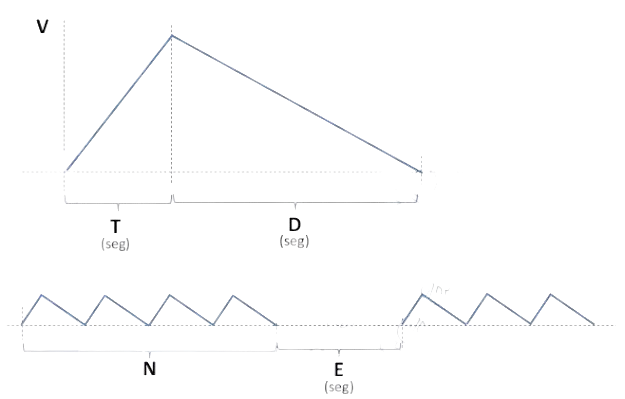
\includegraphics[width = \linewidth]{img/intermitente.png}    
    \caption{Perfil de velocidad de una formación en modo intermitente}
    \label{fig:intermitente}
\end{figure}    

\subsubsection{Comunicación con controlador LED}

Para la configuración y utilización del controlador LED AS1115-BSST se utilizaron los detalles de los registros y formatos de escritura de la hoja de datos del producto. La comunicación con el SAL/T se realiza por el protocolo I2C. Al iniciar el controlador, se configuran los registros de modo de operación para configurar el modo normal de operación, se configura el registro que selecciona cuantos de los 8 dígitos disponibles a controlar se van a utilizar con el valor máximo, ya que se utilizan los primeros 4 dígitos para el display de velocidad y los otros, aunque no de manera completa, para alimentar los demás LEDs del panel frontal. También se configura la intensidad en su valor medio para obtener el brillo esperado. \\

El controlador trae opciones de decodificación para dígitos 7 segmentos en formato Code-B o HEX, pero no existe la posibilidad de configurarlo solo para los primeros 4 dígitos y utilizar los otros segmentos de manera individual. Por esto, es que se desactivó la decodificación en todos los dígitos y se dejó del lado del MCU la transformación de los números a los segmentos de cada dígito correspondientes.  \\ 


El SAL/T, en cada ciclo de operación, releva los valores correspondientes para el display de velocidad y para cada uno de los LEDs indicativos del panel frontal. Luego, transforma estos estados en los bits que corresponden en cada uno de los 8 registros utilizados del controlador LED y lo envía por I2C para reflejar esos estados en las señales de activación de los LEDs en el panel frontal. 


\subsubsection{Registro de eventos}

El SAL/T tiene la capacidad de registrar eventos tanto de manera local como de manera remota. Localmente, interactúa con la tarjeta SD conectada por interfaz SPI y ante cada evento registrable, se escribe dentro de un archivo de logueo donde se va acumulando el histórico de eventos. A nivel remoto, para cada evento, se utiliza la comunicación UART con el módulo ESP32 para que este luego retransmita el mensaje al broker MQTT en el \textit{topic} de logs, y la central operativa pueda recibir estos eventos en tiempo real y almacenarlos en una base de datos propia. \\

Todos los eventos registrados están acompañados de una marca de tiempo que lleva internamente el SAL/T. Cada 10 segundos, el ESP32 envía una actualización de la fecha y hora para que el SAL/T se pueda sincronizar en caso de reinicio o eventual desfasaje del reloj interno. \\ 

El SAL/T registra cualquier evento de cambio de estado que pueda detectar. Algunos de ellos son los siguientes: 
\begin{itemize}
    \item Detección de alimentación tras reinicio
    \item Cambio de estado en la medición de algún SIS
    \item Cambios de estado en la activación del aislamiento de algún SIS
    \item Cambio de estado de modo del sistema
    \item Cambio de zona de circulación
    \item Cambio de estado de la conexión GPS
    \item Cambio de fuente de medición de velocidad
    \item Cambio de velocidad en modo aislado limitado    
    \item Aplicación de cambios de configuración tras recepción de comando remoto
    \item Aplicación de comando remoto
\end{itemize}

El SAL/T permite la descarga de todos los datos registrados en la tarjeta SD de manera local, conectándose por USB a una comunicación serie 8N1, \textit{baudrate} 115.000 y enviando el comando DOWNLOAD\_LOGS. Como respuesta, se envían secuencialmente todos los datos almacenados en la memoria. Esta opción también es posible de manera remota, enviando desde la central operativa el mismo comando y recibiendo la respuesta por el canal de logs del broker MQTT. 

\newpage
\section{Ensayos y resultados}

\subsection{Banco de pruebas}


Para poder realizar pruebas del SAL/T fue necesario armar un banco de pruebas con componentes, módulos y sistemas externos que permitan simular las condiciones de operación real. En la figura \ref{fig:testbench} se visualiza el banco de pruebas completo que se utilizó para realizar las pruebas del dispositivo. 


\begin{figure}[H]
    \centering
    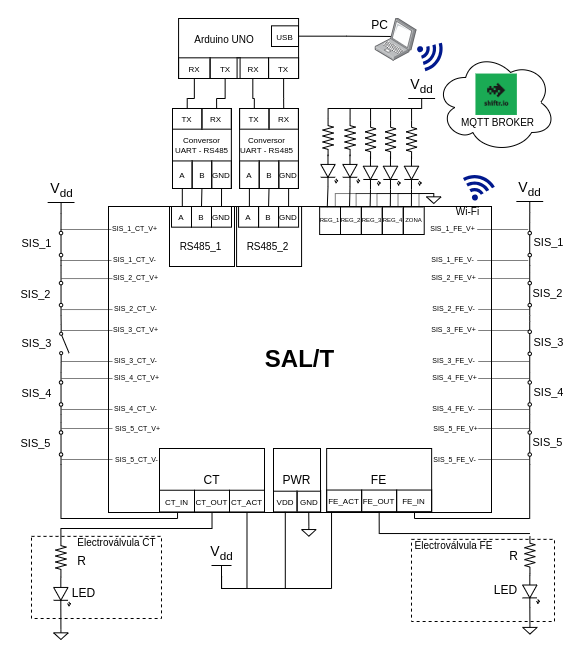
\includegraphics[width = \linewidth]{img/testbench.png}
    \caption{Banco de pruebas completo del SAL/T}
    \label{fig:testbench}
\end{figure}


Los buses de las señales de corte de tracción y freno de emergencia fueron representados cada uno con 5 llaves en serie donde cada una representa la llave de estado de cada SIS. El polo negativo de la llave del último SIS se conecta en la entrada del SAL/T CT\_IN (o FE\_IN para el otro bus). Luego, la salida CT\_OUT (o FE\_OUT) se conecta con la electroválvula correspondiente representada por una resistencia y un LED para visualizar su estado de activación. También se conectó la misma señal de activación que alimenta el bus a la entrada CT\_ACT (o FE\_ACT); en este banco de pruebas, se utilizó una tensión de 5V para alimentar los buses porque facilitó la obtención de la fuente frente a una de 72 VDC o 110 VDC. Sin embargo, mediante el firmware se va a poder compensar esa diferencia en la tensión esperada luego del circuito de medición de los SIS modificando el umbral de los valores esperados en el ADC para determinar si una llave está abierta o cerrada. Por lo tanto, con este esquema se va a poder representar de una manera bastante similar al de operación real, el bus en serie de los SIS que termina en una electroválvula y la intención del SAL/T de intervenir y forzar estados luego de la posible apertura de la línea por alguno de los SIS. \\

Respecto a las salidas de registro de estado del SAL/T y al conector de zona, que permiten la conexión de baja o alta impedancia entre sus 2 terminales dependiendo el estado a reportar, se conectó una resistencia y un LED en un terminal, y conexión a tierra en el otro. Esto se replicó en cada uno de los conectores para poder visualizar el estado reportado a la formación para cada una de las salidas. \\ 


Para simular las comunicaciones con los sistemas de medición de velocidad, se utilizó un Arduino Uno \cite{arduino_uno} y 2 módulos conversores UART - RS485 \cite{conversor_rs485}. El Arduino Uno es una placa de desarrollo basada en el microcontrolador ATmega328P \cite{atmega328}. Cuenta con 14 pines digitales, 6 entradas analógicas, un único puerto UART para comunicación serie, y funciona a 5V con una frecuencia de reloj de 16 MHz. Incluye una interfaz USB para la programación y alimentación, junto con un puerto de alimentación externa. Si bien el Arduino Uno cuenta solo con una interfaz UART, se puede simular una segunda utilizando la librería SoftwareSerial \cite{swSerial} que obtiene resultados suficientes cuando no es necesario realizar una comunicación bidireccional. En la figura \ref{fig:arduino_uno} se visualiza la placa Arduino Uno utilizada. 

\begin{figure}[H]
    \centering
    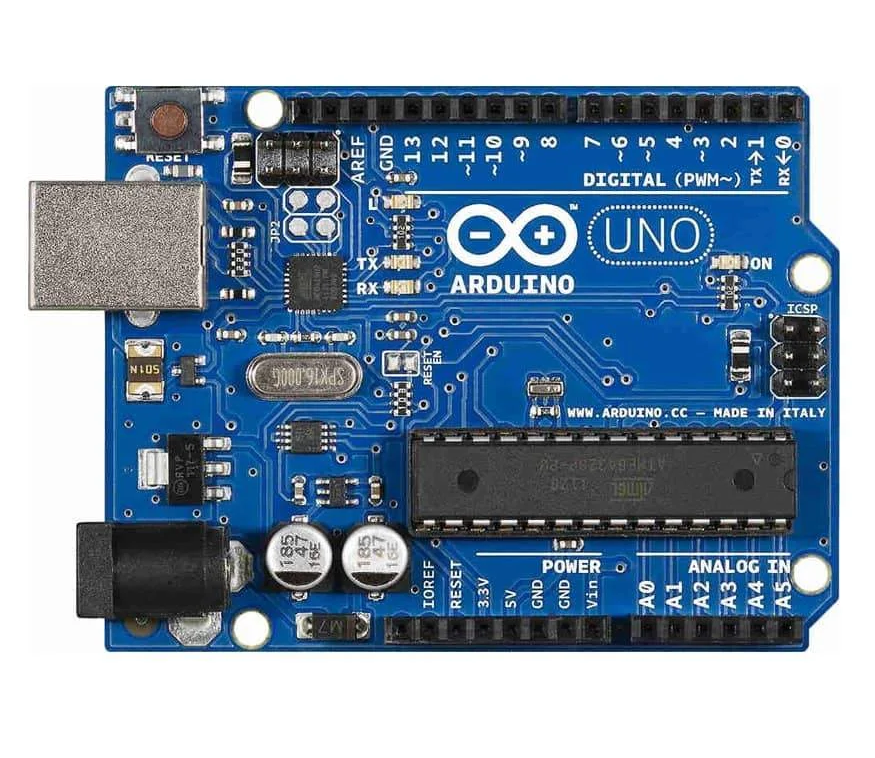
\includegraphics[width = 0.6 \linewidth]{img/arduino_uno.png}
    \caption{Placa de desarrollo Arduino Uno}
    \label{fig:arduino_uno}
\end{figure}


El módulo conversor UART - RS485 utilizado se puede visualizar en la figura \ref{fig:conversor_uart_rs485}; es un módulo fabricado por Hobbytrónica \cite{hobbytronica} basado en el chip MAX485 \cite{max485}; un transceptor de bajo consumo que permite la comunicación serial diferencial a través del protocolo RS485. Este módulo tiene entradas para el lado de la comunicación UART (TX, RX) y un selector para habilitar la trasmisión o la recepción, ya que al pasar a RS485, se convierte en una comunicación half-duplex. Por el lado del RS485, tiene las salidas de A y B esperadas. 


\begin{figure}[H]
    \centering
    \includegraphics[width = 0.5\linewidth]{img/conversor_uart_rs485.png}
    \caption{Módulo conversor UART a RS485}
    \label{fig:conversor_uart_rs485}
\end{figure}

El Arduino va a simular en una de sus interfaces la señal proveniente del Hasler Teloc 1500 generado tramas de 31 bytes iniciadas y terminadas por un byte de start/stop 0x7E y con la información de velocidad en los bytes 7 y 8. En la otra de sus interfaces va a comunicar el valor numérico de la velocidad que trasmitiría el circuito de adaptación e interpretación del generador de impulsos ópticos. Ambas interfaces van a emitir comunicaciones continuas cada 1 segundo con el último valor configurado. \\ 

Por otro lado, el Arduino va a estar conectado a una PC por el conector USB y mediante comunicación serie, va a estar recibiendo los datos de velocidad a transmitir en cada una de sus interfaces. De esta manera, se puede ir variando las velocidades reportadas al SAL/T en cada una de sus interfaces en todo momento desde una PC. \\ 


La PC también va a simular las interacciones de la central operativa conectada al broker MQTT generado con la plataforma shiftr.io \cite{shifrio}; una plataforma en línea que permite visualizar y gestionar flujos de datos en tiempo real mediante el protocolo MQTT. Proporciona un panel interactivo donde se pueden ver en vivo los mensajes publicados y suscritos entre dispositivos, facilitando el monitoreo y depuración de redes IoT. Es fácil de usar y ofrece herramientas para desarrollar, probar y supervisar la comunicación entre dispositivos conectados. Por lo tanto, la PC va a poder enviar comandos remotos al SAL/T a través del broker MQTT y al mismo tiempo va a recibir los mensajes de confirmación de recepción (ACK), los logs del sistema y el reporte periódico del estado del sistema. El SAL/T está configurado para interactuar con el mismo broker MQTT conectándose al servidor a través de la red Wi-Fi que le permite conectarse el módulo interno ESP32. En la figura \ref{fig:shiftrio}
se visualiza el broker shiftr.io con el SAL/T y la central operativa conectados y suscriptos a los distintos \textit{topics} MQTT intercambiando mensajes.



\begin{figure}[H]
    \centering
    \includegraphics[width = \linewidth]{img/shiftrio.png}
    \caption{Visualización de shifr.io conectando el SAL/T con la central operativa}
    \label{fig:shiftrio}
\end{figure}







\subsection{Pruebas de hardware}

Los PCB del SAL/T fueron diseñados para poder ser armados de manera progresiva conectando de a uno los circuitos que interactúan con el MCU. Para eso, se colocó el \textit{footprint} para una resistencia de 0 $\Omega$ o un puente en la alimentación de cada circuito individual. También se colocaron puntos de prueba en casi todas las señales. Esto permitió armar el sistema de manera incremental y asegurándose que cada circuito esté en funcionamiento (a nivel hardware) antes de conectar el siguiente.  \\ 

La primera prueba que se realizó fue conectar la alimentación de uno de los controladores ULN2003 y ejecutar un rutina de activación y desactivación de cada uno de los pines de control utilizados para los relés. Al mismo tiempo, se leía el estado de la salida secundaria del relé para verificar que se produjera el cambio de estado esperado. También se colocó un LED indicativo al lado de cada relé para poder visualizar dentro de la placa el estado de cada uno en estas pruebas. Esta prueba exitosa se repitió para todos los 21 relés del sistema validando que sus circuitos de control, de activación y de salida estuvieran bien conectados y funcionando según lo esperado. \\ 

En segundo lugar, se probaron los circuitos de medición de los SIS. Se alimentó el chip ICL7660AIBAZA y se midió en el punto de prueba de su tensión de salida la tensión esperada de -5V necesaria para alimentar los amplificadores de instrumentación INA823DGKR. Para probar los circuitos de medición, se utilizaron los buses de las señales CT y FE simulados con llaves. Con una rutina de del ADC que leía continuamente los valores en las entradas y la función de \textit{debbuging} que permite hacer una ejecución controlada y visualizar los valores de los registros y utilizando los puntos de prueba sobre la placa, se verificó que los circuitos estén convirtiendo la tensión diferencial entre los terminales de la llave en la tensión \textit{single-ended} esperada. Se probó alimentar los buses con 5V y con 3V3 para verificar que se obtuvieran distintos valores esperados a la salida del circuito y a nivel digital luego del ADC. No se pudo probar los circuitos con alimentación de 72 VDC o 110 VDC pero se validó la línealidad del circuito que permitiría funcionar correctamente para las tensiones diseñadas. \\ 


Luego se probaron los circuitos de control simples con el reset del módulo GPS o la activación del buzzer sonoro en la placa secundaria. En ambos casos, se verificó que el circuito funcionara según lo esperado pudiendo prender y apagar el módulo GPS o el buzzer sonoro con el valor del pin digital al que se conecta el MCU. También se probó la lectura de los circuitos de las llaves de activación de modo aislado limitado, modo aislado total y el botón seleccionador de perfil intermitente obteniendo la tensión esperada en los puntos de prueba y el valor digital en el MCU. \\ 

En cuanto a las interfaces de comunicación entre los distintos módulos o chips del sistema, se hicieron las mediciones de los puntos de prueba básicos con un voltímetro para verificar que las tensiones de reposo de las líneas de comunicación fueran las esperadas. Para los circuitos conversor UART a RS485, se midieron los valores de tensión esperados para las señales A o B utilizando los pines del MCU como salidas GPIO digitales para poder fijar su valor antes de configurarlo para trasmisiones UART. Para los LEDs y display de la placa secundaria, se configuró una rutina que encendía y apagaba progresivamente todos los LEDs disponibles y se verificó visualmente que la conexión sea correcta para cada uno.  








\subsection{Pruebas de firmware}

A nivel firmware, también se realizaron pruebas muy modularizadas para asegurarse el correcto funcionamiento de las interfaces con cada uno de los circuitos o módulos del sistema. \\ 

La comunicación con el módulo GPS se probó inicialmente por fuera del PCB, ya que los módulos (GPS y Nucleo) estaban disponibles antes de la fabricación de la placa. Para esto, se copiaron las conexiones esperadas utilizando cables externos para conectar las interfaces UART de la Nucleo con el módulo GPS. El módulo GPS viene con una configuración por defecto que transmite a un \textit{baudrate} de 9600 una serie de mensajes una vez por segundo. Para verificar la comunicación entre los módulos, del lado del MCU se configuró la recepción por interrupción y se reenviaron todos los datos recibidos a la interfaz de debugging para poder ser inspeccionados. Se observó que efectivamente una vez por segundo se recibían todas las frases NMEA que indicaba la hoja de datos. A partir de esa estructura de datos identificada, se armó un \textit{parser} para poder extraer de la frase GPRMC los datos de estado de la comunicación GPS, la ubicación (latitud, longitud) y la velocidad informada. Estos datos también fueron enviados por la interfaz de debugging para luego verificar si estaban correctos. El módulo GPS puede perder la conexión con los satélites por lo que deja de informar todos los datos así que se probó el estado de conexión correcto y la pérdida de conexión desconectando la antena del sistema. \\ 

Con el módulo ESP32 también se realizaron las primeras pruebas de comunicación de manera externa. El ESP32 cuenta con una interfaz serie accesible mediante USB, por lo que se configuró para retransmitir todo lo recibido por el MCU a través de esta interfaz y también retransmitir lo recibido por USB al MCU. La misma configuración se realizó en el MCU. Por lo tanto, al enviar un mensaje desde la PC al MCU, se recibía por la comunicación con el ESP32 el mismo mensaje, y al enviar desde la PC un mensaje al ESP32, se recibía el mismo mensaje por la interfaz con el MCU. De esta manera, se verificó que la comunicación entre los módulos era correcta y se estaban procesando correctamente los mensajes transmitidos y recibidos. Luego, se configuró el ESP32 para conectarse a una red Wi-Fi y al servidor MQTT, por lo que se modificó el firmware para retransmitir ya no a través de la interfaz USB, sino a través del servidor MQTT. Desde la PC, se configuró el broker MQTT en shifr.io y se conectó como cliente utilizando la librería Paho \cite{paho} de Python para interactuar con el servidor. Con esta extensión, se pudo repetir la prueba de comunicación entre el MCU principal, el ESP32 y el servidor MQTT, ya que los mensajes llegaban correctamente de punta a punta en ambos sentidos. Las conexiones utilizadas para este último escenario se pueden visualizar en la figura \ref{fig:mqtt_testbench} 


\begin{figure}[H]
    \centering
    \includegraphics[width = 0.7\linewidth]{img/mqtt_testbench.png}
    \caption{Conexiones para prueba de comunicación con ESP32 y servidor MQTT}
    \label{fig:mqtt_testbench}
\end{figure}

Para el código del ESP32, también se realizó la prueba de configurarle la conexión a dos redes Wi-Fi y cuando no se pueda conectar a una, intentar la conexión con la otra de manera sistemática. Se levantaron dos redes Wi-Fi y se probó que al desconectar una, se conecta con la otra (envía un log al servidor MQTT cuando se conecta a una nueva red) y al desconectarse ambas se queda monitoreando qué red se levanta primero para establecer una conexión lo antes posible. \\ 

Para la comunicación con la memoria SD, también se logró realizar algunas pruebas anticipadas a tener la placa lista. Para esto, se utilizó un módulo para memorias microSD \cite{modulo_sd} reutilizado de otro proyecto que se puede observar en la figura \ref{fig:modulo_sd}. Este módulo permite conectar solo las señales de SPI con cables externos a la placa Núcleo. Se realizó esta conexión y se probaron algunas funciones básicas de la comunicación como listar los archivos disponibles dentro de la unidad, escribir en un archivo y leer el contenido de un archivo. Con estas pruebas básicas y el desarrollo de las funciones para interactuar, se verificó el funcionamiento en la comunicación por SPI con la memoria SD. Una vez recibidas las placas, se realizaron las mismas pruebas, pero utilizando el zócalo para la memoria microSD soldado a la placa principal junto a las resistencias diseñadas para las lineas de comunicación. 

\begin{figure}[H]
    \centering
    \includegraphics[width = 0.4\linewidth]{img/modulo_sd.jpg}
    \caption{Módulo SD para pruebas de comunicación}
    \label{fig:modulo_sd}
\end{figure}

Para la comunicación con las fuentes de velocidades externas, se utilizó un Arduino Uno y módulos conversor UART a RS-485 para poder conectar con el SAL/T. En estas comunicaciones, se configuró el Arduino para transmitir de manera continua distintas velocidades en el formato esperado de cada uno de los sistemas que simula. Para el generado de impulsos ópticos, se envía el dato numérico de la velocidad directo, y para la señal proveniente del Hasler Teloc 1500 se envía una trama de 31 bytes con el dato de velocidad en los bytes 7 y 8. Del lado del SAL/T, se conectan las interfaces RS-485 con el pin de selección de dirección de la comunicación en modo recepción y se procesan los mensajes recibidos y se envían por interfaz de debugging para visualizarlos desde una PC. En ambas comunicaciones se logró obtener el dato de la velocidad transmitido y asociado a la interfaz del cual proviene cada dato. \\ 

Por último, se realizaron varias pruebas de comunicación y configuración con el controlador LED. Una vez con las placas armadas, ya que el empaquetado del chip no permitía una conexión con cables externos, se realizaron algunas pruebas utilizando el protocolo I2C. Utilizando la hoja de datos como referencia, se escribieron algunos registros para validar la comunicación y el funcionamiento deseado del controlador LED y de los LEDs conectados. Primero se habilitaron todos los dígitos que puede controlar el chip y se fueron encendiendo uno a uno los segmentos y LEDs conectados en un orden específico. Esto permitió verificar el mapeo entre las variables que representan un estado y la posición dentro de un registro del controlador. Una vez validado el mapeo, se armaron alguna funciones que permiten escribir los registros del controlador LED solamente utilizando el estado de los LEDs individuales y el número a mostrar para los dígitos 7 segmentos. De esta manera, se hicieron varias pruebas de escribir todas las cifras en el display y de encender y apagar todos los estados visualizables para verlo reflejado en los LEDs de la placa secundaria. También se probó la escritura de registros de configuración como el ajuste del brillo o la deshabilitación de alguno de los dígitos controlados o el reset por software que permite el controlador. 
\subsection{Pruebas integrales}

Para realizar las pruebas integrales del sistema, se montaron todas las placas, conexiones internas, memorias y se utilizó el banco de pruebas completo de la figura \ref{fig:testbench}. Se cargó en el MCU principal el firmware completo del sistema utilizando todos los mecanismos de RTOS, sincronización, lectura de entradas, activación de salidas y comunicación descriptas previamente. Dentro del módulo ESP32 también se cargó la versión final del firmware que permite la conexión a dos redes Wi-Fi de manera alternada ante una caída de la red actual, conectarse al servidor MQTT suscribiendo y publicando en sus canales e interactuando con el MCU principal por su interfaz serie; también envía un comando de actualización de la fecha y hora de manera periódica después de consultarlo con un servidor NTP. \\

Para estructurar las pruebas integrales del sistema se siguieron punto a punto los requerimientos establecidos para armar un plan de pruebas que permita validarlo de manera completa. Si bien hay requerimientos que pueden estar cubiertos en más de una prueba, se aseguró que todos los requerimientos están cubiertos en al menos una prueba y, por lo tanto, el éxito de todas las pruebas asegura el cumplimiento de todos los requerimientos. \\ 

\paragraph{Prueba 1: Lectura de estado de los SIS}
\begin{enumerate}
\item	Se enciende el SAL/T en estado normal.
\item	Se verifica que se haya activado el relé de registro correspondiente a la correcta alimentación del SAL/T.
\item	Se abre una llave de una señal CT o FE de un SIS.
\item	Se verifica que se encienda el LED rojo de falla del SIS correspondiente.
\item	Se cierra la llave abierta.
\item	Se verifica que se restaure el LED verde de estado normal del SIS correspondiente.
\item	Se repite la prueba hasta agotar las llaves.
\item	Se desconecta la alimentación del SAL/T.
\item	Se verifica que se haya desactivado el relé de registro de alimentación del SAL/T.
\end{enumerate}

\paragraph{Prueba 2: Aislamiento SIS en modo aislado limitado}
\begin{enumerate}
\item	Se enciende el SAL/T en estado normal.
\item	Se transmite una velocidad continua de 10 km/h por debajo de cualquier umbral configurado.
\item	Se abre una llave de una señal X (CT o FE) de un SIS N (1 al 5).
\item	Se verifica que se encienda el LED de falla del SIS correspondiente.
\item	Se verifica que el LED que representa la electroválvula de la señal X se haya apagado por la apertura de la llave.
\item	Se activa la llave local de modo aislado limitado.
\item	Se verifica que se haya encendido el LED del modo aislado limitado en el panel frontal.
\item	Se verifica que se haya activado el relé de registro correspondiente al evento modo aislado limitado.
\item	Se verifica que se haya activado el relé de aislamiento del SIS N para la señal X.
\item	Se verifica que el LED que representa la electroválvula de la señal X se haya encendido por la continuidad de la línea.
\item	Se desactiva la llave de modo aislado limitado retornando al estado normal.
\item	Se verifica que se haya desactivado el relé de registro correspondiente al evento modo aislado limitado.
\item	Se verifica que el aislamiento del SIS no exista más.
\item	Se cierra la llave del SIS abierta.
\item	Se repite la prueba hasta cubrir todas las llaves de los SIS.

\end{enumerate}

\paragraph{Prueba 3: Activación modo total}
\begin{enumerate}
\item	Se enciende el SAL/T en estado normal.
\item	Se transmite una velocidad continua de 10 km/h por debajo de cualquier umbral configurado.
\item	Se abre una llave de una señal X (CT o FE) de un SIS N (1 al 5).
\item	Se verifica que se encienda el LED de falla del SIS correspondiente.
\item	Se verifica que el LED que representa la electroválvula de la señal X se haya apagado por la apertura de la llave.
\item	Se activa la llave local de modo aislado total.
\item	Se verifica que los circuitos de CT y FE haya activado el bypass de las señales conectando las señales ACT con OUT de cada una.
\item	Se verifica que el LED que representa la electroválvula de la señal de CT y de FE se haya encendido por la continuidad forzada de las líneas.
\item	Se transmite una velocidad continua de 50 km/h por encima de los umbrales configurados por otros modos.
\item	Se verifica que el SAL/T no contempla la velocidad y mantiene alimentadas las señales de CT y FE.
\item	Se desactiva la llave de modo aislado total.
\item	Se verifica la liberación de las señales de CT y FE.
\item	Se verifica que la línea de la señal X está interrumpida porque todavía existe una falla en el SIS N.

\end{enumerate}

\paragraph{Prueba 4: Priorización de fuentes de medición de velocidad}
\begin{enumerate}
\item	Se enciende el SAL/T en estado normal.
\item	Se transmite una velocidad continua de 10 km/h por debajo de cualquier umbral configurado en ambas interfaces RS-485.
\item	Se verifica que el display del panel frontal indique la misma velocidad.
\item	Se transmite una velocidad de 20 km/h reportada por la interfaz RS-485\_2 (menor prioridad).
\item	Se verifica que el display del panel frontal mantiene la visualización de la velocidad máxima prioridad 10 km/h.
\item	Se varía la velocidad reportada por la interfaz RS-485\_1 (mayor prioridad) a 25 km/h.
\item	Se verifica que el display del panel frontal indique la velocidad de mayor prioridad 25 km/h.
\item	Se desconecta la fuente comunicación de RS-485\_1 de mayor prioridad.
\item	Se verifica que el display del panel frontal indique la velocidad de mayor prioridad disponible 20 km/h.
\item	Se desconecta la fuente comunicación de RS-485\_2 .
\item	Se verifica que el display del panel frontal indique la velocidad obtenida por el módulo GPS (cercano a 0 km/h estando quieto).
\item	Se desconecta la antena de la comunicación GPS.
\item	Se verifica que el display marque la ausencia de fuente de medición de velocidad con guiones en el display.

\end{enumerate}

\paragraph{Prueba 5: Control de señales críticas ante variación de velocidad}
\begin{enumerate}
\item	Se enciende el SAL/T en estado normal.
\item	Se reconoce la ubicación de la prueba dentro de la zona 1 de circulación según la configuración de los parámetros del GPS.
\item	Se transmite una velocidad continua de 10 km/h por debajo de cualquier umbral configurado en ambas interfaces RS-485.
\item	Se abre una llave de una señal X (CT o FE) de un SIS N (1 al 5).
\item	Se activa la llave local de modo aislado limitado.
\item	Se verifica que el LED que representa la electroválvula de la señal X se haya encendido por la continuidad de la línea producida por el aislamiento del SIS en fallo.
\item	Se verifica que el buzzer sonoro emita sonido de manera intermitente.
\item	Se varía la velocidad reportada por la interfaz RS-485\_1 (mayor prioridad) de manera progresiva hasta alcanzar los 32 km/h.
\item	Se verifica que el display muestra de manera continua la evolución de la velocidad.
\item	Se verifica que al cruzar los 30 km/h (umbral definido para la zona actual como velocidad límite para desaceleración) se interrumpe la señal de CT.
\item	Se verifica que el LED que representa la electroválvula de la señal CT se haya apagado por la interrupción de la línea.
\item	Se verifica que el LED indicativo de corte en la señal de CT se haya encendido.
\item	Se verifica que se haya activado el relé de registro correspondiente a la interrupción de la señal de CT.
\item 	Se verifica que el buzzer sonoro emita sonido de manera continua.
\item	Se disminuye progresivamente la velocidad hasta llegar a los 20 km/h.
\item	Se verifica que al cruzar los 24 km/h (umbral definido para la zona actual como velocidad límite para retomar la aceleración) se libera la señal de CT.
\item	Se verifica que el LED que representa la electroválvula de la señal CT se haya encendido por la restauración de la continuidad de la línea.
\item	Se verifica que el LED indicativo de corte en la señal de CT se haya apagado.
\item	Se verifica que se haya desactivado el relé de registro correspondiente a la interrupción de la señal de CT.
\item	Se verifica que el buzzer sonoro emita sonido de manera intermitente.
\item	Se varía la velocidad reportada por la interfaz RS-485\_1 (mayor prioridad) de manera progresiva hasta alcanzar los 40 km/h.
\item	Se verifica que al cruzar los 30 km/h se interrumpe la señal de CT.
\item	Se verifica que al cruzar los 36 km/h (umbral definido para la zona actual como velocidad límite para frenar) se interrumpe la señal de FE.
\item	Se verifica que el LED que representa la electroválvula de la señal FE se haya apagado por la interrupción de la línea.
\item	Se verifica que el LED indicativo de corte en la señal de FE se haya encendido.
\item	Se verifica que se haya activado el relé de registro correspondiente a la interrupción de la señal de FE.
\item	Se disminuye progresivamente la velocidad hasta llegar a los 0 km/h.
\item	Se verifica que el estado de las señales de CT y FE permanezcan en estado de freno hasta alcanzar los 0 km/h y haber pasado al menos 30 segundos (tiempo mínimo configurado para activar el freno).
\item	Se verifica que transcurridos los 30 segundos y con una velocidad nula, se liberan las señales de CT y FE.
\item	Se verifica que se apaguen los LEDs indicativos de las señales de CT y FE.
\item	Se verifica que se desactiven los relés de registro de CT y FE.

\end{enumerate}

\paragraph{Prueba 6: Modo intermitente}
\begin{enumerate}
\item	Se enciende el SAL/T en estado normal.
\item	Se desconectan o dejan de transmitir todas las mediciones de velocidad.
\item	Se abre una llave de una señal X (CT o FE) de un SIS N (1 al 5).
\item	Se activa la llave local de modo aislado limitado.
\item	Se verifica que se haya aplicado el aislamiento de la llave del SIS N en la línea X.
\item	Se verifica que se hayan activado las señales de CT y FE  durante 30 segundos por la falta de referencia de velocidad.
\item	Se verifica que se ejecute la rutina de modo intermitente para el perfil 1 seleccionado (T=15, D=30, N=4, E=40) durante algunos ciclos.
\item	Se modifica el perfil del modo intermitente con el botón de cambio de perfil al perfil 3.
\item	Se verifica que el LED indicador del perfil seleccionado se desplace cada vez que el botón se presione hasta llegar al perfil 3.
\item	Se verifica que se ejecute la rutina de modo intermitente para el perfil 3 seleccionado (T=30, D=60, N=3, E=60) durante algunos ciclos.

\end{enumerate}

\paragraph{Prueba 7: Comandos remotos para cambio de modo}
\begin{enumerate}
\item	Para cada comando que se envía dese la central operativa, se antepone un ID generado y se verifica la recepción de una confirmación del mensaje (ACK) para el mismo ID.
\item	Se envía desde la central operativa un comando PARADA\_TOTAL de manera periódica cada 1 segundo durante 60 segundos.
\item	Se verifica que se haya encendido el LED de presencia de comando remoto en el panel frontal.
\item	Se verifica que se hayan interrumpido las señales de CT y FE.
\item	Se verifica que después de 10 segundos después de finalizada la última transmisión, el sistema vuelve al estado normal y apaga el LED de presencia comando remoto.
\item	Se abre la llave de un SIS N en la línea de FE.
\item	Se envía desde la central operativa un comando COCHE\_DERIVA de manera periódica cada 1 segundo.
\item	Se verifica que se haya interrumpido las señales de CT y liberado la de FE.
\item	Se envía el comando CANCEL una única vez y se deja de transmitir el comando anterior.
\item	Se verifica que el sistema vuelve al estado normal.
\item	Se abre la llave de un SIS N en la línea de CT.
\item	Se envía desde la central operativa un comando AISLADO\_TOTAL de manera periódica cada 1 segundo durante 60 segundos.
\item	Se verifica que se hayan liberado las señales de CT y de FE.
\item	Se verifica que después de 10 segundos después de finalizada la última transmisión, el sistema vuelve al estado normal.
\item	Se envía el comando COMMAND\_VALIDITY\_CONFIG:20.
\item	Se envía el comando INTERMITENTE:1 de manera periódica durante 120 segundos.
\item	Se verifica que el sistema entró en modo intermitente con el perfil 1 seleccionado ejecutando la rutina configurada (T=15, D=30, N=4, E=40).
\item	Se verifica que después de 20 segundos después de finalizada la última transmisión (valor configurado), el sistema vuelve al estado normal.
\item	Se envía el comando INTERMITENTE\_CONFIG:4,20,40,5,60).
\item	Se envía el comando INTERMITENTE:4 de manera periódica durante 120 segundos.
\item	Se verifica que el sistema entró en modo intermitente con el perfil 4 seleccionado ejecutando la rutina con los parámetros configurados (T=20, D=40, N=5, E=60).
\item	Se verifica que después de 20 segundos después de finalizada la última transmisión (valor configurado), el sistema vuelve al estado normal.

\end{enumerate}

\paragraph{Prueba 8 - Registro de eventos}
\begin{enumerate}
\item	Se enciende el SAL/T en estado normal.
\item	Para todos los mensajes de logueos, se verifica que la fecha y hora registrada sea correcta.
\item	Se verifica durante toda la prueba que el sistema reporte por el canal de STATUS de MQQT el estado actual del sistema.
\item	Se abren varias llaves de un SIS N para la línea X (CT o FE).
\item	Se verifica la recepción del cambio de estado de cada llave en el canal de logs de MQTT desde la central operativa.
\item	Se activa el modo aislado limitado y se verifica el reporte de cambio de modo.
\item	Se verifica el reporte de la acción de aislamiento de los SIS intervenidos.
\item	Se pierde la fuente de medición RS-485\_1 de velocidad y se verifica el reporte de cambio de fuente de velocidad a la siguiente disponible.
\item	Se pierden todas las fuentes de velocidad por lo que se activa el modo intermitente y se verifica el reporte de cambio de modo de operación.
\item	Se verifica que se reporte cada activación y desactivación de las señales CT y FE.
\item	Se restaura las fuentes de velocidad y se verifica el reporte del cambio de modo.
\item	Se varía la velocidad y se verifica el reporte de las velocidades transcurridas en modo aislado limitado.
\item	Se activa la llave de modo aislado total y se verifica el reporte del cambio de modo.
\item	Se verifica el reporte de desintervención de los SIS afectados ya el SAL/T controla las señales de CT Y FE directamente.
\item	Se desactivan las llaves MAL y MAT para restablecer el modo normal y se verifica el reporte de cambio de modo.
\item	Se desconecta la antena GPS y se verifica que se reporte la perdida de cobertura y referencia de zona.
\item	Se reconecta la antena GPS y se verifica el reporte de cobertura y referencia de zona 1.
\item	Se envía el comando DOWNLOAD\_LOGS desde la central operativa y se verifica la recepción de todos los eventos transmitidos previamente con la fecha y hora originales de los eventos.
\item	Se conecta una PC por USB al SAL/T por comunicación serie, se envía de manera local el comando DOWNLOAD\_LOGS y se verifica la recepción de todos los eventos transmitidos previamente con la fecha y hora originales de los eventos.

\end{enumerate}

\paragraph{Prueba 9: Conectividad Wi-Fi}
\begin{enumerate}
\item	Se enciende el SAL/T en estado normal.
\item	Se apaga la red Wi-Fi principal a la que se conecta el sistema.
\item	Se verifica la recepción de un registro de evento de cambio de red a la red secundaria.
\item	Se apaga la red Wi-Fi secundaria a la que se conecta el sistema.
\item	Se verifica que se haya perdido la comunicación con la central operativa.
\item	Se prende cualquiera de las redes Wi-Fi configuradas.
\item	Se verifica que la conexión con la central operativa se restablece en pocos segundos y reporta la red a la que se conectó.

\end{enumerate}




Las pruebas integrales descriptas cubren el 100\% de los requerimientos y se diseñaron de manera temprana en el proceso de desarrollo del firmware. Esto permitió tener claro cuál es el comportamiento esperado del sistema en distintas situaciones e ir escribiendo un firmware que responda a estas pruebas. Luego de varias iteraciones y pruebas, se obtuvo un resultado exitoso en todas las pruebas para la versión final del sistema. 





\newpage
\section{Conclusiones}
\subsection{Conclusiones generales}

En este trabajo se logró diseñar y armar un nuevo prototipo de un sistema de aislado limitado / total que cumple con todos los requerimientos acordados para el proyecto. Esto permite acercar el objetivo de realizar la fabricación de un SAL/T de manera nacional y mejorar la seguridad en la operación de las formaciones ferroviarias causando una mejora directa en la vida de las personas que utilizan este medio de transporte de manera cotidiana. \\

En este prototipo, se implementó un hardware más moderno que su versión anterior, pero sin dejar de reutilizar muchas de sus técnicas de diseño y lógicas de circuito; esto permitió que este prototipo agregue funcionalidades y mejoras sobre el sistema sin dejar de contar con la robustez del prototipo predecesor. En cuanto al firmware, se logró implementar una lógica del sistema utilizando un sistema operativo en tiempo real que permita orquestar de manera eficiente los recursos y los tiempos de respuesta de cada uno de los subsistemas incluidos en el SAL/T. \\ 

Las pruebas integrales realizadas simulando todos los dispositivos externos propios de una formación ferroviaria, permiten confirmar que el prototipo cumple con el comportamiento esperado en todas las situaciones especificadas en los requerimientos. Sin embargo, para poder validar el correcto funcionamiento del sistema en condiciones operativas de una formación ferroviaria, queda pendiente realizar pruebas conectadas a los sistemas reales de uso del SAL/T. Además de las potenciales diferencias con el banco de pruebas utilizado, es esperable que algunas funcionalidades o decisiones de implementación hayan quedado alejadas o diferentes a las imaginadas por el autor del pliego de especificaciones de Trenes Argentinos, ya que durante todo el proyecto no se logró mantener una iteración constante con la empresa para validar las decisiones de diseño y, si bien responde a los requerimientos del pliego, la interpretación de este puede llevar a distintos enfoques o pretensiones. \\ 

La etapa de relevamiento de los requerimientos y definición del alcance del proyecto resultó la etapa más relevante del trabajo porque todas las tareas subsiguientes se desprenden de esta primera etapa. Luego, el diseño de hardware significó la mayor carga de horas de trabajo por su naturaleza de incorporación de todos los requerimientos del proyecto y rigidez que conlleva la fabricación de un hardware incorrecto. Por esto, se hizo una primera etapa de diseño integral de la solución donde se estableció de manera modular los distintos subsistemas del SAL/T y la comunicación de cada uno con el controlador principal. Luego, se diseñaron e implementaron de manera independiente cada uno de los módulos respetando las interfaces definidas previamente. De esta manera, se logró realizar un proceso ordenado de diseño desde lo general a lo particular. \\ 

Este trabajo tiene como mayor aporte la fabricación de un prototipo que considera todos los requerimientos para armar un sistema de seguridad productivo para instalar en las formaciones ferroviarias de la empresa Trenes Argentinos. El detalle de su diseño y consideraciones queda plasmado en este documento lo que permite entender y reutilizar una gran parte del proyecto al momento de realizar una versión productiva. \\

A nivel personal, este trabajo permitió consolidar y poner en práctica de manera integral gran parte de los conocimientos adquiridos durante la carrera de grado de ingeniería electrónica realizando un proyecto que atraviesa las etapas de relevamiento de los requerimientos, diseño de hardware, diseño de firmware, fabricación, implementación, verificación, diseño y ejecución de pruebas y presentación del proyecto mismo.
\input{5 - Conclusiones/5.2 - Próximos pasos}


\newpage

\section{Bibliografía}



 \begin{thebibliography}{30}

 \bibitem{gicsafe}
 \textbf{GICSAFe}. Grupo de Investigación en Calidad y Seguridad de las Aplicaciones Ferroviarias. \href{https://sites.google.com/view/conicet-gicsafe}{https://sites.google.com/view/conicet-gicsafe}.

 
 \bibitem{trenes_arg}
 \textbf{Trenes Argentinos} Trenes Argentinos Operaciones, empresa del estado. \href{https://www.argentina.gob.ar/transporte/trenes-argentinos}{https://www.argentina.gob.ar/transporte/trenes-argentinos}.

  \bibitem{salt_paper}
 \textbf{Supervision system for emergency brake and traction-system isolation on train formations}. Di Vito Iván Mariano, Gomez Pablo Martin, Lutenberg Ariel, 2020. \href{https://ieeexplore.ieee.org/document/9085280}{\textit{https://ieeexplore.ieee.org/document/9085280}}.


\bibitem{salt_ivan}
 \textbf{Aplicación de la técnica de patrones de diseño a la implementación de un Sistema de Aislamiento Limitado/Total ferroviario}. Di Vito, Iván Mariano. 2019 \href{https://bibliotecadigital.fi.uba.ar/items/show/18446}{\textit{https://bibliotecadigital.fi.uba.ar/items/show/18446}}.

 


\bibitem{norma_50126}
\textbf{UNE-EN 50126-1}. Aplicaciones ferroviarias. Especificación y demostración de la fiabilidad, la disponibilidad, la mantenibilidad y la seguridad (RAMS). 2005. \href{https://www.une.org/encuentra-tu-norma/busca-tu-norma/norma?c=N0033106}{https://www.une.org/encuentra-tu-norma/busca-tu-norma/norma?c=N0033106}


 \bibitem{patrones}
 \textbf{Design Patterns for Safety-Critical Embedded Systems}. Ashraf Armoush. RWTH Aachen University. 2010.



 \bibitem{salt_case}
 \textbf{Sistema de supervisión de la seguridad del material ferroviario utilizando patrones de diseño}. Ivan Mariano Di Vito, Pablo Gomez, Ariel Lutenberg, Adrian Laiuppa. 2019. \href{https://drive.google.com/file/d/1FDtRL4We4daZ7XrJ81sL2f6HrZbYlOuG/view}{\textit{https://drive.google.com/file/d/1FDtRL4We4daZ7XrJ81sL2f6HrZbYlOuG/view}}. 

 \bibitem{spec}
 \textbf{SISTEMA DE AISLADO LIMITADO / TOTAL (SAL-T)}. ESPECIFICACIÓN TÉCNICA. Bypass Sistemas Instrumentados de Seguridad a Bordo del Material Rodante ET.SO. No 046 /18 – E3. 2022.

  



\bibitem{norma_61508}
\textbf{UNE-EN 61508-4}. Seguridad funcional de los sistemas eléctricos/electrónicos/electrónicos programables relacionados con la seguridad. Parte 4: Definiciones y abreviaturas. 2011. \href{https://www.une.org/encuentra-tu-norma/busca-tu-norma/norma?c=N0047025}{https://www.une.org/encuentra-tu-norma/busca-tu-norma/norma?c=N0047025} 

\bibitem{norma_ipc2221}
\textbf{IPC-2221}. Estándar genérico sobre la PCB. Revisión C; 2023. \href{https://shop.ipc.org/ipc-2221/ipc-2221-standard-only/Revision-c/english}{https://shop.ipc.org/ipc-2221/ipc-2221-standard-only/Revision-c/english}

\bibitem{norma_50128}
\textbf{UNE-EN 50128}. Aplicaciones ferroviarias. Sistemas de comunicación, señalización y procesamiento. Software para sistemas de control y protección del ferrocarril. 2012. \href{https://www.une.org/encuentra-tu-norma/busca-tu-norma/norma?c=N0049040}{https://www.une.org/encuentra-tu-norma/busca-tu-norma/norma?c=N0049040} 



\bibitem{norma_50129}
\textbf{UNE-EN 50129}. Aplicaciones ferroviarias. Sistemas de comunicación, señalización y procesamiento. Sistemas electrónicos relacionados con la seguridad para la señalización. 2020. \href{https://www.une.org/encuentra-tu-norma/busca-tu-norma/norma?c=N0063513}{https://www.une.org/encuentra-tu-norma/busca-tu-norma/norma?c=N0063513} 




\bibitem{clasificacion_fallas}
\textbf{Random, systematic, and common cause failure: How do you manage them?}. Michela Gentile, Angela E. Summers. 2006. \href{https://sis-tech.com/wp-content/uploads/2005/10/Random_Systematic_and_Common_Cause_Failure.pdf}{https://sis-tech.com/wp-content/uploads/2005/10/Random\_Systematic\_and\_Common\_Cause\_Failure.pdf} 

 \bibitem{nucleo144}
\textbf{STM32 Nucleo-144 development board with STM32F429ZI MCU}. STMicroelectronics. \href{https://www.st.com/en/evaluation-tools/nucleo-f429zi.html}{https://www.st.com/en/evaluation-tools/nucleo-f429zi.html} 

\bibitem{stm32f429zi}
\textbf{STM32F429ZI}. High-performance advanced line, Arm Cortex-M4 core. STMicroelectronics. \href{https://www.st.com/en/microcontrollers-microprocessors/stm32f429zi.html}{https://www.st.com/en/microcontrollers-microprocessors/stm32f429zi.html} 

\bibitem{st_link}
\textbf{ST-LINK/V2-1}. In-Circuit Debugger and Programmer. STMicroelectronics.
\href{https://www.st.com/en/development-tools/st-link-v2.html}{https://www.st.com/en/development-tools/st-link-v2.html}

\bibitem{stCubeIde}
\textbf{STM32CubeIDE}. Free Development Environment for STM32 Microcontrollers. STMicroelectronics.
\href{https://www.st.com/en/development-tools/stm32cubeide.html}{https://www.st.com/en/development-tools/stm32cubeide.html}

\bibitem{stCubeMx}
\textbf{STM32CubeMX}. Initialization Code Generator for STM32 Microcontrollers. STMicroelectronics.
\href{https://www.st.com/en/development-tools/stm32cubemx.html}{https://www.st.com/en/development-tools/stm32cubemx.html}

\bibitem{esp32}
\textbf{ESP32-DevKitC}. Development board from Espressif.  \href{https://docs.espressif.com/projects/esp-dev-kits/en/latest/esp32/esp32-devkitc/index.html}{https://docs.espressif.com/projects/esp-dev-kits/en/latest/esp32/esp32-devkitc/index.html} 

\bibitem{ieee_802.11}
\textbf{IEEE 802.11}. IEEE Computer Society, IEEE Standard for Information Technology—Telecommunications and Information Exchange Between Systems Local and Metropolitan Area Networks—Specific Requirements Part 11: Wireless LAN Medium Access Control (MAC) and Physical Layer (PHY) Specifications, IEEE Standard 802.11-2020, 2021. \href{https://standards.ieee.org/standard/802_11-2020.html}{https://standards.ieee.org/standard/802\_11-2020.html}


\bibitem{bluetooth}
\textbf{Bluetooth}. Bluetooth Core Specification Version 5.4. 2023. \href{https://www.bluetooth.com/specifications/bluetooth-core-specification/}{https://www.bluetooth.com/specifications/bluetooth-core-specification/}

\bibitem{arduino_ide}
\textbf{Arduino IDE}. Open source repository.  \href{https://github.com/arduino/arduino-ide}{https://github.com/arduino/arduino-ide}


\bibitem{esp_ids}
\textbf{ESP-IDS}. Espressif IoT Development Framework.\href{https://idf.espressif.com/}{https://idf.espressif.com/}

\bibitem{platformio}
\textbf{PlatformIO}. Cross-platform, cross-architecture, multiple framework, professional tool for embedded systems designers. \href{https://platformio.org/}{https://platformio.org/}


\bibitem{gy-neo6}
\textbf{Modulo GPS GY-NEO6MV2}. Módulo basado en NEO-6M. \href{https://www.todomicro.com.ar/ARDUINO/339-modulo-gps-gy-neo6mv2-con-antena.html}{https://www.todomicro.com.ar/ARDUINO/339-modulo-gps-gy-neo6mv2-con-antena.html}


\bibitem{neo6}
\textbf{NEO-6M}. Módulo GNSS / GPS. Ublox. \href{https://www.u-blox.com/en/product/neo-6-series}{https://www.u-blox.com/en/product/neo-6-series}


\bibitem{mqtt_ibm}
\textbf{Getting to know MQTT}. Michael Yuan. 2021. \href{https://developer.ibm.com/articles/iot-mqtt-why-good-for-iot/}{https://developer.ibm.com/articles/iot-mqtt-why-good-for-iot/}

\bibitem{mqtt_img}
\textbf{What is MQTT}. Tobias Goebel
Twilion. 2023. \href{https://www.twilio.com/en-us/blog/what-is-mqtt}{https://www.twilio.com/en-us/blog/what-is-mqtt}


\bibitem{wifi_security}
\textbf{Wi-Fi Security}. Wi-Fi Alliance, Wi-Fi Security Technologies: WEP, WPA, and WPA2. \href{https://www.wi-fi.org/discover-wi-fi/security}{https://www.wi-fi.org/discover-wi-fi/security}

\bibitem{wifi_img}
\textbf{Wi-Fi Direct}. Wikipedia. \href{https://en.wikipedia.org/wiki/Wi-Fi_Direct}{https://en.wikipedia.org/wiki/Wi-Fi\_Direct}


\bibitem{gps}
\textbf{GPS}. U.S. Department of Defense, Global Positioning System Standard Positioning Service Performance Standard, 4th ed. 2008. \href{https://www.gps.gov/technical/ps/}{https://www.gps.gov/technical/ps/}

\bibitem{gps_img}
\textbf{Cómo funcionan los dispositivos GPS? Trilateración vs Triangulación}.Gabri. Arcgeek. 2018.  \href{https://acolita.com/como-funcionan-los-dispositivos-gps-trilateracion-vs-triangulacion/}{https://acolita.com/como-funcionan-los-dispositivos-gps-trilateracion-vs-triangulacion/}



\bibitem{rs485}
\textbf{Texas Instruments, RS-485}: Theory and Application, Application Report SLAA070D. 2004. \href{https://www.ti.com/lit/an/slaa070d/slaa070d.pdf}{https://www.ti.com/lit/an/slaa070d/slaa070d.pdf}

\bibitem{rtos}
\textbf{What is a Real-Time Operating System (RTOS)?} Digikey article. 2021. \href{https://www.digikey.com/en/maker/projects/what-is-a-realtime-operating-system-rtos/28d8087f53844decafa5000d89608016}{https://www.digikey.com/en/maker/projects/what-is-a-realtime-operating-system-rtos/28d8087f53844decafa5000d89608016}



\bibitem{hasler}
\textbf{Hasler Rail}. Speed Sensing and Odometry. 2016
\href{https://www.haslerrail.com/wp-content/uploads/2019/03/HaslerRail_DataRecordingSafety_EN_v1.pdf}{https://www.haslerrail.com/wp-content/uploads/2019/03/HaslerRail\_DataRecordingSafety\_EN\_v1.pdf}

\bibitem{mouser}
\textbf{Mouser Electronics}.  Global distributor of semiconductors and electronic components. \href{https://www.mouser.com/}{https://www.mouser.com/}

\bibitem{digikey}
\textbf{DigiKey Corporation}. Global distributor of semiconductors and electronic components. \href{https://www.digikey.com/}{https://www.digikey.com/}


\bibitem{kicad}
\textbf{KiCad EDA}. Version 6. KiCad Developers.
\href{https://www.kicad.org/}{https://www.kicad.org/}


\bibitem{LTspice}
\textbf{LTSpice.} Free SPICE simulator. Analog devices.
\href{https://www.analog.com/en/resources/design-tools-and-calculators/ltspice-simulator.html}{https://www.analog.com/en/resources/design-tools-and-calculators/ltspice-simulator.html}


\bibitem{github}
\textbf{GitHub, Inc.}. A Platform for Version Control and Collaboration,
\href{https://github.com}{https://github.com}


\bibitem{git}
\textbf{Git} A Distributed Version Control System. Linus Torvalds. 2005.
\href{https://git-scm.com}{https://git-scm.com}


\bibitem{repo}
\textbf{martinanus/salt} Repositorio de firmware y hardware del proyecto. Martín Anús. 2024. \href{https://github.com/martinanus/salt}{https://github.com/martinanus/salt}



\bibitem{INA823DGKR}
\textbf{INA823DGKR}. Texas Instruments. Instrumentation Amplifiers Precision. 
\href{https://www.ti.com/lit/gpn/ina823}{https://www.ti.com/lit/gpn/ina823}


\bibitem{ICL7660AIBAZA}
\textbf{ICL7660AIBAZA}. Renesas. Switching Voltage Regulators. 
\href{https://ar.mouser.com/datasheet/2/698/REN_icl7660s_a_DST_20200210-1997724.pdf}{https://ar.mouser.com/datasheet/2/698/REN\_icl7660s\_a\_DST\_20200210-1997724.pdf}

\bibitem{JW2SN-DC5V}
\textbf{JW2SN-DC5V}. Panasonic Industrial Devices. General Purpose Relays 5A 5VDC DPDT SEALED PCB. 
\href{https://ar.mouser.com/manufacturer/panasonic-industrial-devices/}{https://ar.mouser.com/manufacturer/panasonic-industrial-devices/}


\bibitem{V23047A1005A501}
\textbf{V23047A1005A501}. TE Connectivity. Safety Relays 2 CO CONTACTS 5VDC
\href{https://ar.mouser.com/datasheet/2/418/6/ENG_DS_SR2M_0820-735797.pdf}{https://ar.mouser.com/datasheet/2/418/6/ENG\_DS\_SR2M\_0820-735797.pdf}

\bibitem{norma_61810}
\textbf{UNE-EN 61810-3}. Relés electromecánicos elementales. Parte 3: Relés con contactos guiados (unidos mecánicamente). 2015. 
\href{https://www.une.org/encuentra-tu-norma/busca-tu-norma/norma?c=N0054926}{https://www.une.org/encuentra-tu-norma/busca-tu-norma/norma?c=N0054926}


\bibitem{rele_img}
\textbf{Relay Terminology}. Altech Corp.
\href{https://oylair.com/wp-content/uploads/2021/03/resources-library-3-relay-terminology.pdf}{https://oylair.com/wp-content/uploads/2021/03/resources-library-3-relay-terminology.pdf}


\bibitem{ULN2003D1013TR}
\textbf{ULN2003D1013TR}- STMicroelectronics. Darlington Transistors Seven NPN Array.
\href{https://ar.mouser.com/datasheet/2/389/uln2001-1852702.pdf}{https://ar.mouser.com/datasheet/2/389/uln2001-1852702.pdf}

\bibitem{darlington}
\textbf{Darlington’s Contributions to Transistor Circuit Design} David A. Hodges, Fellow, IEEE. 1999.
\href{https://people.eecs.berkeley.edu/~hodges/DarlingtonCircuit.pdf}{https://people.eecs.berkeley.edu/~hodges/DarlingtonCircuit.pdf}


\bibitem{registrador_eventos}
\textbf{Use of Event Data Recorders in Rail Transit}. Federal Transit Administration, , FTA Report No. 0123. 2015.
\href{https://www.transit.dot.gov/research-innovation/use-event-data-recorders-rail-transit}{https://www.transit.dot.gov/research-innovation/use-event-data-recorders-rail-transit}

\bibitem{llave_elibet}
\textbf{Interruptor Bipolar 20A de 2 posiciones}. Elibet. Serie LI. 
\href{https://www.elibet.com/wp-content/uploads/2014/08/Elibet-20A.pdf}{https://www.elibet.com/wp-content/uploads/2014/08/Elibet-20A.pdf}

\bibitem{indicador_velocidad}
\textbf{Data Recording and Safety}. Hasler Rail. \href{http://www.iotrains.com/fileadmin/user_upload/04_DataRecording.pdf}{http://www.iotrains.com/fileadmin/ user\_upload/04\_DataRecording.pdf}

\bibitem{crc}
\textbf{Catalogue of parametrised CRC algorithms with 16 bits}. Greg Cook. 
\href{http://reveng.sourceforge.net/crc-catalogue/16.htm}{http://reveng.sourceforge.net/crc-catalogue/16.htm}


\bibitem{edu-ciaa}
\textbf{EDU-CIAA-NXP}. Información general de la placa de desarrollo EDU-CIAA-NXP desarrollada por el proyecto CIAA (Computadora Industrial Abierta Argentina). \href{https://www.proyecto-ciaa.com.ar/devwiki/doku.php%3Fid=desarrollo:edu-ciaa:edu-ciaa-nxp.html}{https://www.proyecto-ciaa.com.ar/devwiki/doku.php\%3Fid=desarrollo:edu-ciaa:edu-ciaa-nxp.html}

\bibitem{SN65HVD1176DR}
\textbf{SN65HVD1176DR}. Texas Instruments. CI interfaz RS-485 PROFIBUS RS-485 Transceiver. 
\href{https://www.ti.com/lit/gpn/sn65hvd1176}{https://www.ti.com/lit/gpn/sn65hvd1176}

\bibitem{profibus}
\textbf{Profibus International}. PROFIBUS Technology Overview.
\href{https://www.profibus.com/technologies/profibus}{https://www.profibus.com/technologies/profibus}

\bibitem{SZP6SMB12CAT3G}
\textbf{SZP6SMB12CAT3G}. Littelfuse. ESD Protection Diodes / TVS Diodes.
\href{https://www.littelfuse.com/media?resourcetype=datasheets&itemid=a54ab340-efe4-40d7-99cb-dd80d69f6f3a&filename=littelfuse_tvs_diode_szp6smb_datasheet.pdf}{https://www.littelfuse.com/media?resourcetype=datasheets\&itemid=a54ab340-efe4-40d7-99cb-dd80d69f6f3a\&filename=littelfuse\_tvs\_diode\_szp6smb\_datasheet.pdf}


\bibitem{MF-USMF020-2}
\textbf{MF-USMF020-2}. Bourns. Resettable Fuses.
\href{https://www.mouser.co.uk/datasheet/2/54/mfusmf-777646.pdf}{https://www.mouser.co.uk/datasheet/2/54/mfusmf-777646.pdf}


\bibitem{SI2343DS-T1-E3}
\textbf{SI2343DS-T1-E3}. Vishay Semiconductors. MOSFETs 30V 4.0A 1.25W 53 mohms @ 10V. 
\href{https://www.vishay.com/doc?72079}{https://www.vishay.com/doc?72079}

\bibitem{87583-2010BLF}
\textbf{87583-2010BLF}. Amphenol FCI. USB Connectors 4P RECEPTACLE TYPE A.
\href{https://www.mouser.co.uk/datasheet/2/18/1/87583-2579162.pdf}{https://www.mouser.co.uk/datasheet/2/18/1/87583-2579162.pdf}

\bibitem{altanet}
\textbf{Módem router Portátil USB 4G LTE Wi-Fi}. Altanet.
\href{https://www.voipexperts.com.ar/productos/routers/routers-4g/alta-stick-st10.html}{https://www.voipexperts.com.ar/productos/routers/routers-4g/alta-stick-st10.html}


\bibitem{DM3AT-SF-PEJM5}
\textbf{DM3AT-SF-PEJM5}. Hirose Connector. Memory Card Connectors R/A SMT MICROSD CON PUSH-PUSH.
\href{https://www.mouser.co.uk/datasheet/2/185/DM3AT_SF_PEJM5_CL0609_0031_0_00_2DDrawing_00009471-1614303.pdf}{https://www.mouser.co.uk/datasheet/2/185/ DM3AT\_SF\_PEJM5\_CL0609\_0031\_0\_00\_2DDrawing\_00009471-1614303.pdf}


\bibitem{sd_sandisk}
\textbf{Micro SD Ultra 8GB Class 10}. SanDisk.
\href{https://dcpsoltec.mercadoshops.com.ar/MLA-1346308183-micro-sd-sandisk-ultra-8gb-clase-10-_JM}{https://dcpsoltec.mercadoshops.com.ar/MLA-1346308183-micro-sd-sandisk-ultra-8gb-clase-10-\_JM}

\bibitem{AS1115-BSST}
\textbf{AS1115-BSST}. ams OSRAM. LED Display Drivers LED Driver with Keyscan.
\href{https://www.mouser.co.uk/datasheet/2/588/asset_pdf_25493045-3432722.pdf}{https://www.mouser.co.uk/datasheet/2/588/asset\_pdf\_25493045-3432722.pdf}

\bibitem{WP154A4SEJ3VBDZGW/CA}
\textbf{WP154A4SEJ3VBDZGW/CA}. Kingbright. Standard LEDs - Through Hole 5MM RGB LED.
\href{https://www.mouser.co.uk/datasheet/2/216/WP154A4SEJ3VBDZGW_CA-1145236.pdf}{https://www.mouser.co.uk/datasheet/2/216/WP154A4SEJ3VBDZGW\_CA-1145236.pdf}


\bibitem{WP7113LZGCK}
\textbf{WP7113LZGCK}. Kingbright. Standard LEDs - Through Hole 5MM LOW CURRENT GREEN LED.
\href{https://www.mouser.co.uk/datasheet/2/216/WP7113LZGCK-535810.pdf}{https://www.mouser.co.uk/datasheet/2/216/WP7113LZGCK-535810.pdf}

\bibitem{LTC-5723HR}
\textbf{LTC-5723HR}. Lite-On. LED Displays and Accessories 4 Digit, Red. 
\href{https://www.mouser.co.uk/datasheet/2/239/C5723HR-1141844.pdf}{https://www.mouser.co.uk/datasheet/2/239/C5723HR-1141844.pdf}

\bibitem{1543-650-149}
\textbf{1543-650-149}. Bourns. Pushbutton Switches Push Switch.
\href{https://www.mouser.co.uk/datasheet/2/54/1543-55078.pdf}{https://www.mouser.co.uk/datasheet/2/54/1543-55078.pdf}

\bibitem{CEM-1205-IC}
\textbf{CEM-1205-IC}. Same Sky.Piezo Buzzers and Audio Indicators buzzer 5V, driving circuit.
\href{https://www.mouser.co.uk/datasheet/2/1628/cem_1205_ic-3509057.pdf}{https://www.mouser.co.uk/datasheet/2/1628/cem\_1205\_ic-3509057.pdf}


\bibitem{NVTR0202PLT1G}
\textbf{NVTR0202PLT1G}. onsemi. MOSFETs PFET 20V 0.4A 80MOH.
\href{https://www.mouser.co.uk/datasheet/2/308/1/NTR0202PL_D-2319410.pdf}{https://www.mouser.co.uk/datasheet/2/308/1/NTR0202PL\_D-2319410.pdf}


\bibitem{jlcway}
\textbf{JLCWAY}.PCB Manufacturing and Assembly Services.
\href{https://jlcpcb.com}{https://jlcpcb.com}

\bibitem{labi_3d}
\textbf{Impresiones 3D}. Laboratorio Abierto de la Facultad de Ingeniería de la Universidad de Buenos Aires.
\href{https://labi.fi.uba.ar/impresiones-3d}{https://labi.fi.uba.ar/impresiones-3d}

\bibitem{gabinete}
\textbf{Caja estanca plástica 310x310x110 Blanca IP65}. Sistelectric de Genros.
\href{https://sistelectric.com/producto/06313111g/caja-estanca-plastica-310x310x110-gris-ip65/}{https://sistelectric.com/producto/06313111g/caja-estanca-plastica-310x310x110-gris-ip65/}


\bibitem{freertos}
\textbf{FreeRTOS}. Real-Time Operating System for Embedded Devices.
\href{https://www.freertos.org}{https://www.freertos.org}




\bibitem{nmea}
\textbf{GPS - NMEA sentence information}. Glenn Baddeley. 2001.
\href{https://aprs.gids.nl/nmea/}{https://aprs.gids.nl/nmea/}

\bibitem{ntp}
\textbf{NTP Server} The NTP Pool Project
\href{https://www.pool.ntp.org}{https://www.pool.ntp.org}


\bibitem{shifrio}
\textbf{shiftr.io}. MQTT Broker and Dataflow Visualizer
\href{https://www.shiftr.io}{https://www.shiftr.io}

\bibitem{arduino_uno}
\textbf{Arduino}. Arduino Uno Rev3.
\href{https://docs.arduino.cc/hardware/uno-rev3/}{https://docs.arduino.cc/hardware/uno-rev3/}

\bibitem{conversor_rs485}
\textbf{Modulo Conversor Rs485 Ttl Max485 Transceiver}. Hobbytronica. 
\href{https://www.hobbytronica.com.ar/MLA-1412581125-x5-modulo-conversor-rs485-ttl-max485-transceiver-arduino-_JM}{https://www.hobbytronica.com.ar/MLA-1412581125-x5-modulo-conversor-rs485-ttl-max485-transceiver-arduino-\_JM}

\bibitem{atmega328}
\textbf{ATMega328-p}. 8-bit AVR Microcontroller. Microchip Technology Inc. 
\href{https://www.microchip.com/wwwproducts/en/ATmega328p}{https://www.microchip.com/wwwproducts/en/ATmega328p}

\bibitem{swSerial}
\textbf{Software Serial Library}. Arduino. 
\href{https://docs.arduino.cc/learn/built-in-libraries/software-serial/}{https://docs.arduino.cc/learn/built-in-libraries/software-serial/}


\bibitem{hobbytronica}
\textbf{Hobbytrónica}. Casa de electrónica y robótica. 
\href{https://docs.arduino.cc/learn/built-in-libraries/software-serial/}{https://www.hobbytronica.com.ar/}

\bibitem{max485}
\textbf{MAX485}. Low-Power, Slew-Rate-Limited RS-485/RS-422 Transceivers. Analog devices.
\href{https://www.analog.com/en/products/max485.html}{https://www.analog.com/en/products/max485.html}

\bibitem{paho}
\textbf{Paho MQTT Python Client Library}. Eclipse Foundation. 
\href{https://eclipse.dev/paho/}{https://eclipse.dev/paho/}


\bibitem{modulo_sd}
\textbf{Modulo lector de tarjetas SD}. Electrouno. 
\href{https://www.unoelectro.com.ar/MLA-864661170-modulo-lector-de-tarjetas-micro-sd-arduino-unoelectro-_JM}{https://www.unoelectro.com.ar/MLA-864661170-modulo-lector-de-tarjetas-micro-sd-arduino-unoelectro-\_JM}




 \end{thebibliography}

\end{document}